
\chapter{Quark Gluon Analysis}
\label{ch:quark_gluon_analysis}
\epigraph{\textit{``Research is what I am doing I don't know know what I'm doing.''}}{---  Wernher von Braun}

\newthought{In this chapter}, the analysis of quarks and gluons is presented. The overall goal with this analysis is to improve the knowledge of gluon jets by developing a method to increase the precision at which quark and gluon jets can be distinguished. The overall goal is to improve the understanding af gluon hadronization and splitting by measuring the gluon hadronization in 3-jet events and the gluon splitting in 4-jet events.
The method includes two models; a $b$-tagging model which tag individual jets within an event, and a $g$-tagging models which classify entire events. 


This chapter is organized as follows. In section \autoref{sec:q:data_preprocessing}, the applied datasets are presented and the initial selection criteria for the data are described. Visualizations of the most important variables for the quark and gluon jet events are shown in section \autoref{sec:q:EDA}. The choices of loss and evaluation function are discussed in \autoref{sec:q:loss_evaluation_function}. In \autoref{sec:q:b_tagging_analysis}, the developed $b$-tagging model is presented, and measures of the model's efficiency are shown in section \autoref{sec:q:b_tagging_effiency}. Similarly, the $g$-tagging model is presented in section \autoref{sec:q:g_tagging_analysis}, and measures of the model's efficiency are shown in \autoref{sec:q:g_tagging_effiency}. The jet hadronization in 3-jet events is analyzed in \autoref{sec:q:generalized_angularities_3j} and the gluon splitting in 4-jet events in \autoref{sec:q:gluon_splitting_4j}. Finally the quark gluon project is discussed in \autoref{sec:q:discussion} and concluded in \autoref{sec:q:conclusion}.


% \newthought{The analysis} of the quarks and gluons that were introduced in the previous chapter is described here. The overall goal is to be able to discriminate between quark and gluon jets to better be able to describe the gluon jets. The gluon jet distributions are measured in 3-jet events and how they split in 4-jet events. This chapter is organized as follows. In \autoref{sec:q:data_preprocessing} the data are presented and the initial cuts are described and the variables are visualized in \autoref{sec:q:EDA}. The choices of loss and evaluation function are discussed in \autoref{sec:q:loss_evaluation_function}. In \autoref{sec:q:b_tagging_analysis} the first of the two overall models developed in this chapter is presented, the $b$-tagging model. The efficiency of this model is measured in \autoref{sec:q:b_tagging_effiency}. The second model, the $g$-tagging model is used for classification of entire events, compared to the $b$-tagging model which classifies individual jets, and is introduced in \autoref{sec:q:g_tagging_analysis} and its efficiency is measured in \autoref{sec:q:g_tagging_effiency}. The jet distributions in 3-jet events are analyzed in \autoref{sec:q:generalized_angularities_3j} and their the gluon splitting in 4-jet events in \autoref{sec:q:gluon_splitting_4j}. Finally the quark gluon project is discussed in \autoref{sec:q:discussion}.


\section{Data Preprocessing}
\label{sec:q:data_preprocessing}

The data files were acquired from Prof. Peter Hansen (NBI) who worked on the ALEPH experiment. The Data\sidenote{Remember that \q{Data} refers to actual measurements, whereas \q{data} refers to any data (not necessarily real-life data).} consists of \num{43} data files from between \num{1991} and \num{1995} totalling \SI{3.5}{\giga\byte} (Data). In addition to the datasets measured by the ALEPH experiment, Monte Carlo (MC) simulations of events containing quark and gluon jets are applied. These additional simulations total \num{125} files (\SI{8.4}{\giga\byte}) and additional \num{42} MC-files with only $b$\=/quark events (MCb) (\SI{2.1}{\giga\byte}). The data files which are in the form of \emph{Ntuples}, ROOT's data format \autocite{brunROOTObjectOriented1997}, are converted to HDF5-files by using the Python package uproot \autocite{ScikithepUproot2019}. While iterating over the Ntuples, some basic selection criteria are applied before exporting the data to HDF5-format. 

The first selection criteria is that the center of mass energy $E$ of the events has to be close the mass of the Z boson, ${\SI{90.8}{\GeV} \leq E \leq \SI{91.6}{\GeV}}$. The second selection criteria is used to remove ${Z \rightarrow \tau^+ \tau^-}$ events by requiring that the sum of the momenta in each event is greater or equal to \SI{32}{\GeV}. The third selection criteria is used to select events of high quality by requiring at least two good tracks in the events to ensure a primary vertex, where a good track is defined as having at least \num{7} TPC hits and \num{1} silicon hit or more. Finally it is required that the cosine of the thrust axis polar angle, which is the angle between the trust axis and the beam, is less than or equal to \num{0.8} to avoid any low angle events since the detector performance worsens significantly in that region. These initial requirements were standard requirements for the ALEPH experiment.
% (P. Hansen, personal communication, December, 2019).

An additional selection criteria was applied to further improve the quality of the applied data by defining a lower threshold value for \emph{jet matching}. The jet matching is the process of matching the jet with one of the final state quarks. The jet is said to be matched if the dot product between the final quark momentum and the jet momentum is higher than the threshold value. A high jet matching threshold results in events with cleaner jets but at the expense of less statistics. A jet matching threshold of \num{0.90} was found to be a good compromise between purity and quantity where \SI{97.8}{\percent} of all 2-jet events are matched and \SI{96.7}{\percent} of all events with more than two jets were matched\sidenote{Compare this to \SI{98.5}{\percent} and \SI{97.8}{\percent} for a threshold of \num{0.85} or \SI{95.9}{\percent} and \SI{93.9}{\percent} for a threshold of \num{0.95}.}.  

The structure of the data contained in Ntuples is quite different compared to the \q{normal}  structure of tidy data \autocite{JSSv059i10}. The data is organized such that one iterates over each event where the variables are variable-length depending on the number of jets in the events; this is also known as \emph{jagged} arrays. The data is un-jagged\sidenote{Such that e.g. a 3-jet event will figure as three rows in the dataset.} before exporting to HDF5-format and only the needed variables are kept. This reduces the total output file to a \SI{2.9}{\giga\byte} HDF5-file including both Data, MC, and MCb. The number of events for each number of jets can be seen in Table~\ref{tab:q:datasize}.

\begin{margintable}[1cm]
  \centering
  \begin{tabular}{@{}rrr@{}}
  $n$-jet &    Data     &   MC  \\
  \midrule
  \num{2}     &  \num{1179869} &  \num{3646797}  \\
  \num{3}     &  \num{1206430} &  \num{3593630}  \\
  \num{4}     &   \num{213584} &   \num{560477}  \\
  \num{5}     &    \num{10555} &    \num{20764}  \\
  \num{6}     &       \num{85} &      \num{98}  \\
  Total       &  \num{2610523} &  \num{7821766}  \\  
  \end{tabular}
  \vspace{2mm}
  \caption{The number of $n$-jet events for Data and MC.}
  \label{tab:q:datasize}
  \vspace{\abovecaptionskip}
\end{margintable}

\FloatBarrier
\section{Exploratory Data Analysis} \label{sec:q:EDA}

The variables applied in the machine learning models are the three vertex variables \code{projet}, \code{bqvjet}, and \code{ptljet}, which were introduced in \autoref{ch:hep:particle_physcis_LEP}, these variables are the primary focus of this section. 
For MC-simulated data, both the final state particles are simulated as well as the trajectories of the particles within the detector and the detector interactions. This means, that for MC-simulated data the detector measurements can be directly compared to the \q{true} particles. For the MC simulated data, each event is generated such that the type of collision, or \emph{flavor}, is known and assigned the variable \code{flevt}. The mapping from flavor to \code{flevt} can be seen in Table~\ref{tab:q:flavor_to_flevt}.
\begin{margintable}
  \centering
  \begin{tabular}{@{}rccccc@{}}
  Flavor: & $bb$ & $cc$ & $ss$ & $dd$ & $uu$  \\
  \code{flevt}: & \num{5} & \num{4} & \num{3} & \num{2} & \num{1}  
  \end{tabular}
  \vspace{2mm}
  \caption[Mapping Between the Flavor and the Variable Flevt]{Mapping between the flavor and the variable \code{flevt}.}
  \label{tab:q:flavor_to_flevt}
\end{margintable}

Unfortunately the truth information about the individual jets in the event is not recorded in the MC files, only the information about which type of quarks were created in the collision and not which jets corresponds to which quarks. We define that an event is \emph{$q$\=/matched} if one, and only one, of the jets are assigned to one of the (final) quarks, if one, and only one, of the jets are assigned to the other (final) quark, and if no other jets are matched to any of the (final) quarks. We then define what constitutes a $b$\=/jet: if it has \code{flevt} $= 5$, the entire event is $q$\=/matched, and the jet is matched to one of the (final) quarks. Similarly, $c$\=/jets and $uds$\=/jets are defined using the same range of requirements as $b$\=/jets with the only change that $\code{flevt}=4$ for a $c$\=/jet and \code{flevt} $\in \{1, 2, 3\}$ for a $uds$\=/jet. 

A gluon jet is defined to be a jet in a (any-flavor) $q$\=/matched event where the jet itself is not assigned to any of the (final) quarks. Strictly speaking, this means that the gluon jet is not \SI{100}{\percent} certain of being a gluon. We cannot know this, as not all of the input parameters in the MC simulation are known, only the final clustered jets. Due to the $q$\=/match criterion this also means that some jets are assigned the label \q{non\=/$q$\=/matched} for which these jets are regarded as background. The distribution of different types of jets can be seen in Table~\ref{tab:q:flevt_overview} and shown as relative numbers in Table~\ref{tab:q:flevt_overview_percent_relative}.
% \vspace{-2mm}
\begin{table}[h!]
  \centering
  \begin{tabular}{@{}rrrrrr@{}}
    $n$    & \multicolumn{1}{c}{$b$} & \multicolumn{1}{c}{$c$} & \multicolumn{1}{c}{$uds / l$} & \multicolumn{1}{c}{$g$} & non\=/$q$\=/matched    \\ 
    \midrule
    \num{2}     & \num{2713454} &  \num{944380} & \num{2125900} &       \num{0} & \num{1509860} \\
    \num{3}     & \num{2433878} &  \num{964212} & \num{2129218} & \num{3365969} & \num{1887613} \\
    \num{4}     &  \num{326264} &  \num{156332} &  \num{336548} & \num{1012198} &  \num{410566} \\
    \num{5}     &   \num{10332} &    \num{5960} &   \num{12668} &   \num{54525} &   \num{20335} \\
    \num{6}     &      \num{42} &      \num{26} &      \num{52} &     \num{320} &     \num{148} \\
    \midrule
    Total & \num{5483970} & \num{2070910} & \num{4433012} & \num{4604386} & \num{3828522} \\
  \end{tabular}
  \caption[Number of Different Types of Jets for MC and MCb for $n$-Jet Events]{Number of different types of jets for MC and MCb for $n$-jet events. See also Table~\ref{tab:q:flevt_overview_percent_relative} for relative numbers.}
  \label{tab:q:flevt_overview}
\end{table}
% \vspace{-3mm}

Applying the criteria defined above for what constitutes a specific type of jet, the 1D-distributions for the three vertex variables are plotted in Figure~\ref{fig:q:vertex_variables}. 
% For all three subplots the histograms are shown with logarithmic $y$\=/axes, all $b$\=/jets in blue, $c$\=/jets in red, $g$\=/jets in green, and all of the jets (no matter their type) are shown in orange. The distributions for 2-jet events are shown in fully opaque color, 3-jet events in dashed lines, and 4-jet events in lighter colors. 
% In the left subplot the \code{projet} variable is plotted where it can be seen that high values of \code{projet} tend to indicate $b$\=/jets. 
The left subplot shows that high values of \code{projet} tend to indicate $b$\=/jets. 
In the middle subplot \code{bqvjet} is plotted which shares many similarities with the \code{projet} variables, including that high values indicate $b$\=/jets. In the right subplot the \code{ptljet} is plotted. This variable has many zeros in it which correlates mostly with gluons\sidenote{Around \SI{98}{\percent} of all $g$\=/jets are zeros for the variable \code{ptljet} compared to $\sim \SI{82}{\percent}$ for $c$\=/jets and $\sim \SI{70}{\percent}$ for $b$\=/jets.} and large values are mostly due to $b$\=/jets. 

Furthermore, Figure~\ref{fig:q:vertex_variables} shows that there are minor differences between the variables when comparing 2-, 3-, and 4-jet events, except for 2-jet events which do not contain any gluons at all. 

% In general it is clear to see how the differences in distribution between the \num{2}-, \num{3}-, and \num{4}-jet events are minor, with the one exception of \num{2}-jet events which does not contain any gluons at all. 

\begin{figure*}[h!]
  \centerfloat
  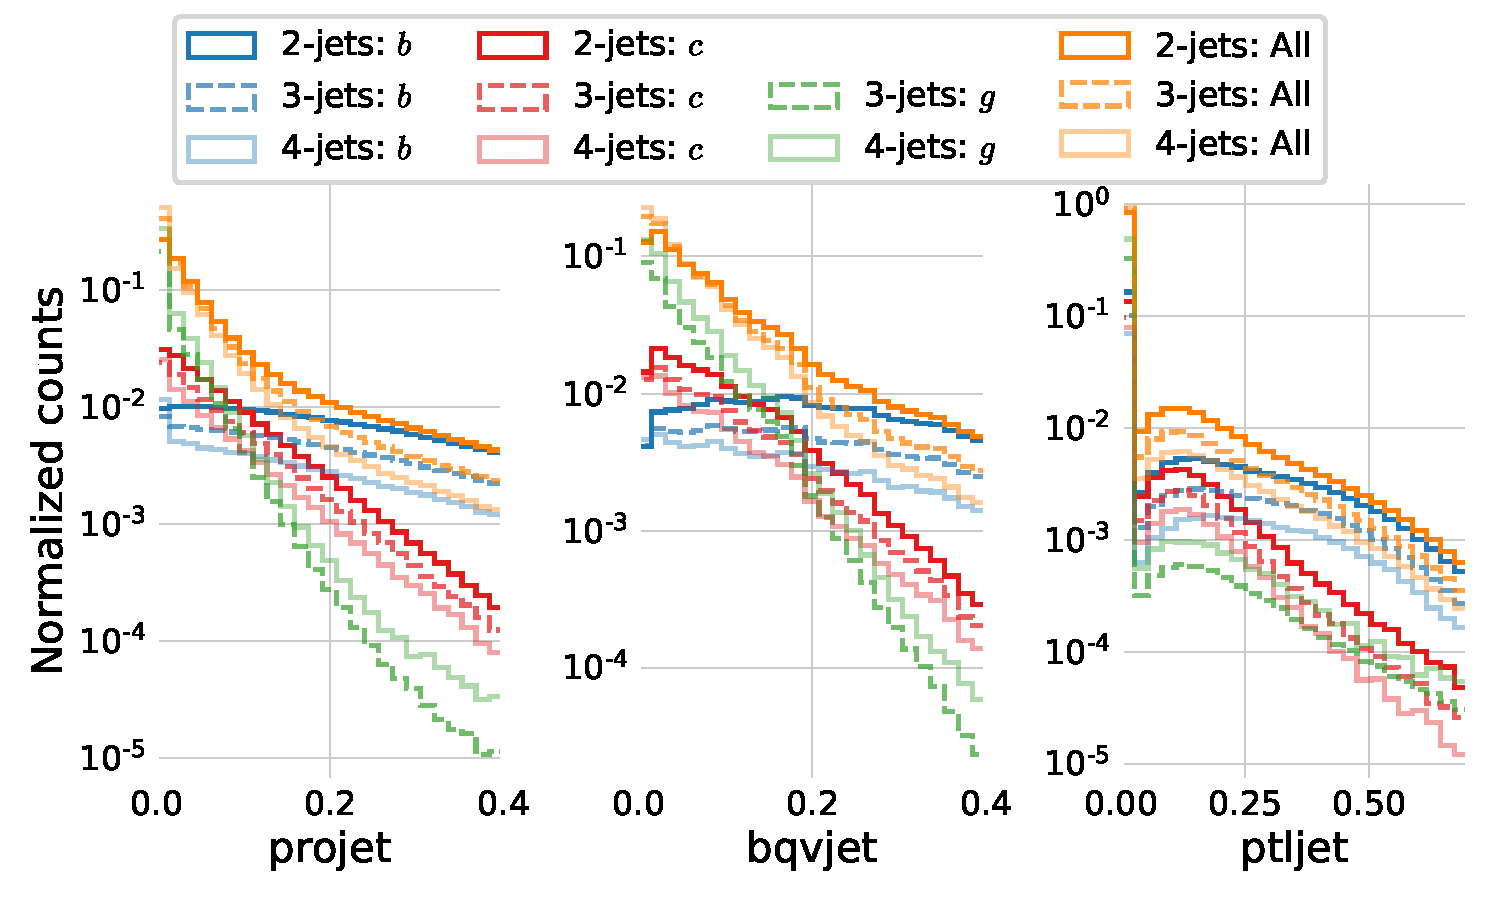
\includegraphics[width=1\textwidth, trim=10 10 5 5, clip]{figures/quarks/btagging_variables_hist-down_sample=1.00-ML_vars=vertex-selection=b-ejet_min=4-n_iter_RS_lgb=99-n_iter_RS_xgb=9-cdot_cut=0.90-version=19.pdf}
  \caption[Histograms of the Vertex Variables]
          {Normalized histograms of the three vertex variables: \code{projet}, \code{bqvjet}, and \code{ptljet}. In blue colors the variables are shown for \textcolor{blue}{true b-jets}, in red for \textcolor{red}{true c-jets}, in green for \textcolor{green}{true g-jets}, and in orange for \textcolor{orange}{all of the jets} (including non q-matched). In fully opaque color are shown the distributions for 2-jet events, in dashed (and lighter color) 3-jet events, and in semi-transparent 4-jet events. Notice the logarithmic y-axis, that there are no g-jets for 2-jet events (as expected), and that all of the distributions are very similar no matter how many jets.
          } 
  \label{fig:q:vertex_variables}
\end{figure*}

\FloatBarrier
\subsection{Dimensionality Reduction}

Even though only three vertex variables are applied, it is be difficult to evolve a good understanding of how well the variables can separate different kinds of jets. The dataset contains millions of events, so a simple 3D scatter plot quickly becomes overcrowded and hard to interpret. In order to improve the visualization of the applied data, dimensionality reduction is used to reduce the three dimensions down to two dimensions. 

Within recent years the field of dimensionality reduction algorithms has grown a lot from just the typical (linear) principal component analysis to also include nonlinear algorithms. The t-SNE algorithm \autocite{maatenVisualizingDataUsing2008} deserves an honorable mention since this algorithm revolutionized the usage of (nonlinear) dimensionality reduction algorithms in e.g. bioinformatics \citep{toghieshghiQuantitativeComparisonConventional2019, wallachProteinSmallmoleculeDatabase2009}  yet its mathematical foundation has strongly been improved with the newer, faster UMAP algorithm \autocite{mcinnesUMAPUniformManifold2018} which usage is also expanding \citep{bechtEvaluationUMAPAlternative2018, bechtDimensionalityReductionVisualizing2019, diaz-papkovichUMAPRevealsCryptic2019}. 

The aim of UMAP, short for Uniform Manifold Approximation and Projection, is to correctly identify and preserve the structure, or topology, of the high-dimensional feature space in a lower-dimensional output space. In order to optimally preserve both the global and local structure of the data, the algorithm stitch together local manifolds in the high-dimensional feature space such that the difference between the high- and low-dimensional representations is minimized according to the cross-entropy \citep{mcinnesUMAPUniformManifold2018}. Compared to t-SNE the approach in UMAP has a topological background compared to the more heuristic approach taken by t-SNE. 

The UMAP algorithm has several hyperparameters, where two of the most important ones are the number of neighbors \code{n_neighbors} which controls the priority between correctly preserving the global versus the local structure, and the \code{min_dist} which defines how tightly together UMAP is allowed to cluster the points in the low-dimensional representation. In order to determine the best combination of \code{n_neighbors} and \code{min_dist} a grid search with \code{n_neighbors} ${\in \{10, 50, 100, 250 \}}$ and \code{min_dist}$\in \{0, 0.2, 0.5\}$ is performed. This is shown for 4-jet events in Figure~\ref{fig:q:UMAP_vertex_all_4j}. 

\begin{marginfigure}
  \centerfloat
  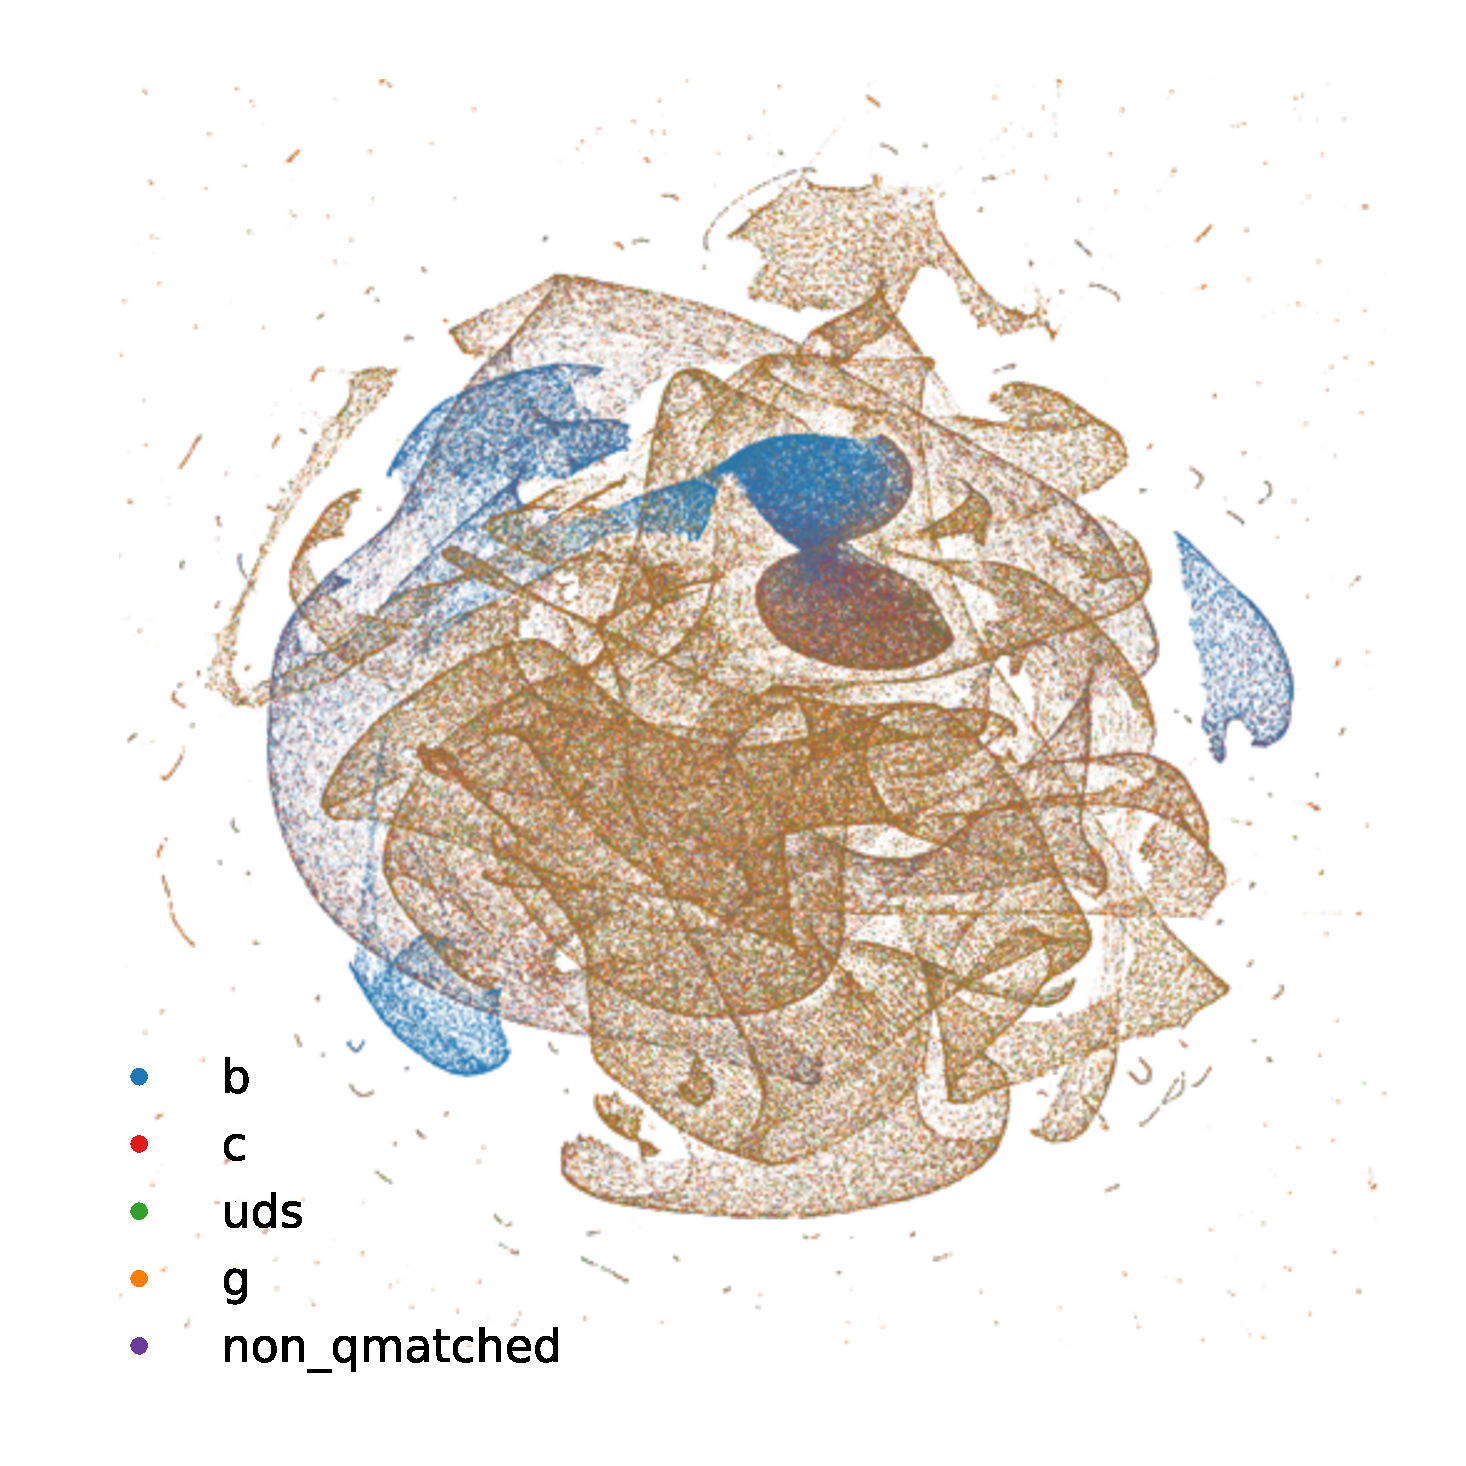
\includegraphics[draft=false, width=0.95\textwidth, trim=50 45 50 50, clip]{figures/quarks/df_UMAP-X=1120952-n_neighbors=250-min_dist=0.2-metric=euclidean-input2b_njet=4_algorithm=UMAP_single.pdf}
  \vspace{1mm}
  \caption[UMAP Visualization of the Vertex Variables for 4-Jet Events]
          {Visualization of the vertex variables in 4-jet events for the different categories: \textcolor{blue}{true b-jets} in blue, \textcolor{red}{true c-jets} in red, \textcolor{green}{true uds-jets} in green, \textcolor{orange}{true g-jets} in orange, and \textcolor{purple}{non q-matched} events in purple. The clustering is performed with the UMAP algorithm which outputs a 2D-projection. This projection is then visualized using the Datashader which takes care of point size, avoids over and underplotting, and color intensity.} 
  \label{fig:q:UMAP_vertex_4j}
  \vspace{5mm}
\end{marginfigure}

The best combination of \code{n_neighbors} and \code{min_dist} is subjective at best, but I judged that $\code{n_neighbors}=250$ and $\code{min_dist}=0.2$ gave the best compromise between preserving local and global structure. The results of running UMAP on 4-jet events can be seen in Figure~\ref{fig:q:UMAP_vertex_4j}. Note that the UMAP algorithm is not provided any information about which jets are which types or any other truth information, that information is only provided afterwards to the actual plot. Here the millions of points are plotted using Datashader \autocite{bednarDatashaderRevealingStructure2019} to avoid overplotting and colored according to the jet type. The figure shows that there are some clear $b$\=/jet clusters, however, most of the data seem to be a mix of $g$\=/ and $uds$\=/jets. 

Similarly, Figure~\ref{fig:q:UMAP_vertex_3j} 
% and \ref{fig:q:UMAP_vertex_2j} 
show the two-dimensional visualization for 3-jet events correspondingly. These three figures suggest that it should be possible to discriminate the $b$\=/jets from the other jets somewhat, however, no clear separation is expected. The t-SNE algorithm was also tested but showed inferior performance compared to UMAP, see Figure~\ref{fig:q:tsne_vertex} for an example of this.

\begin{marginfigure}
  \centerfloat
  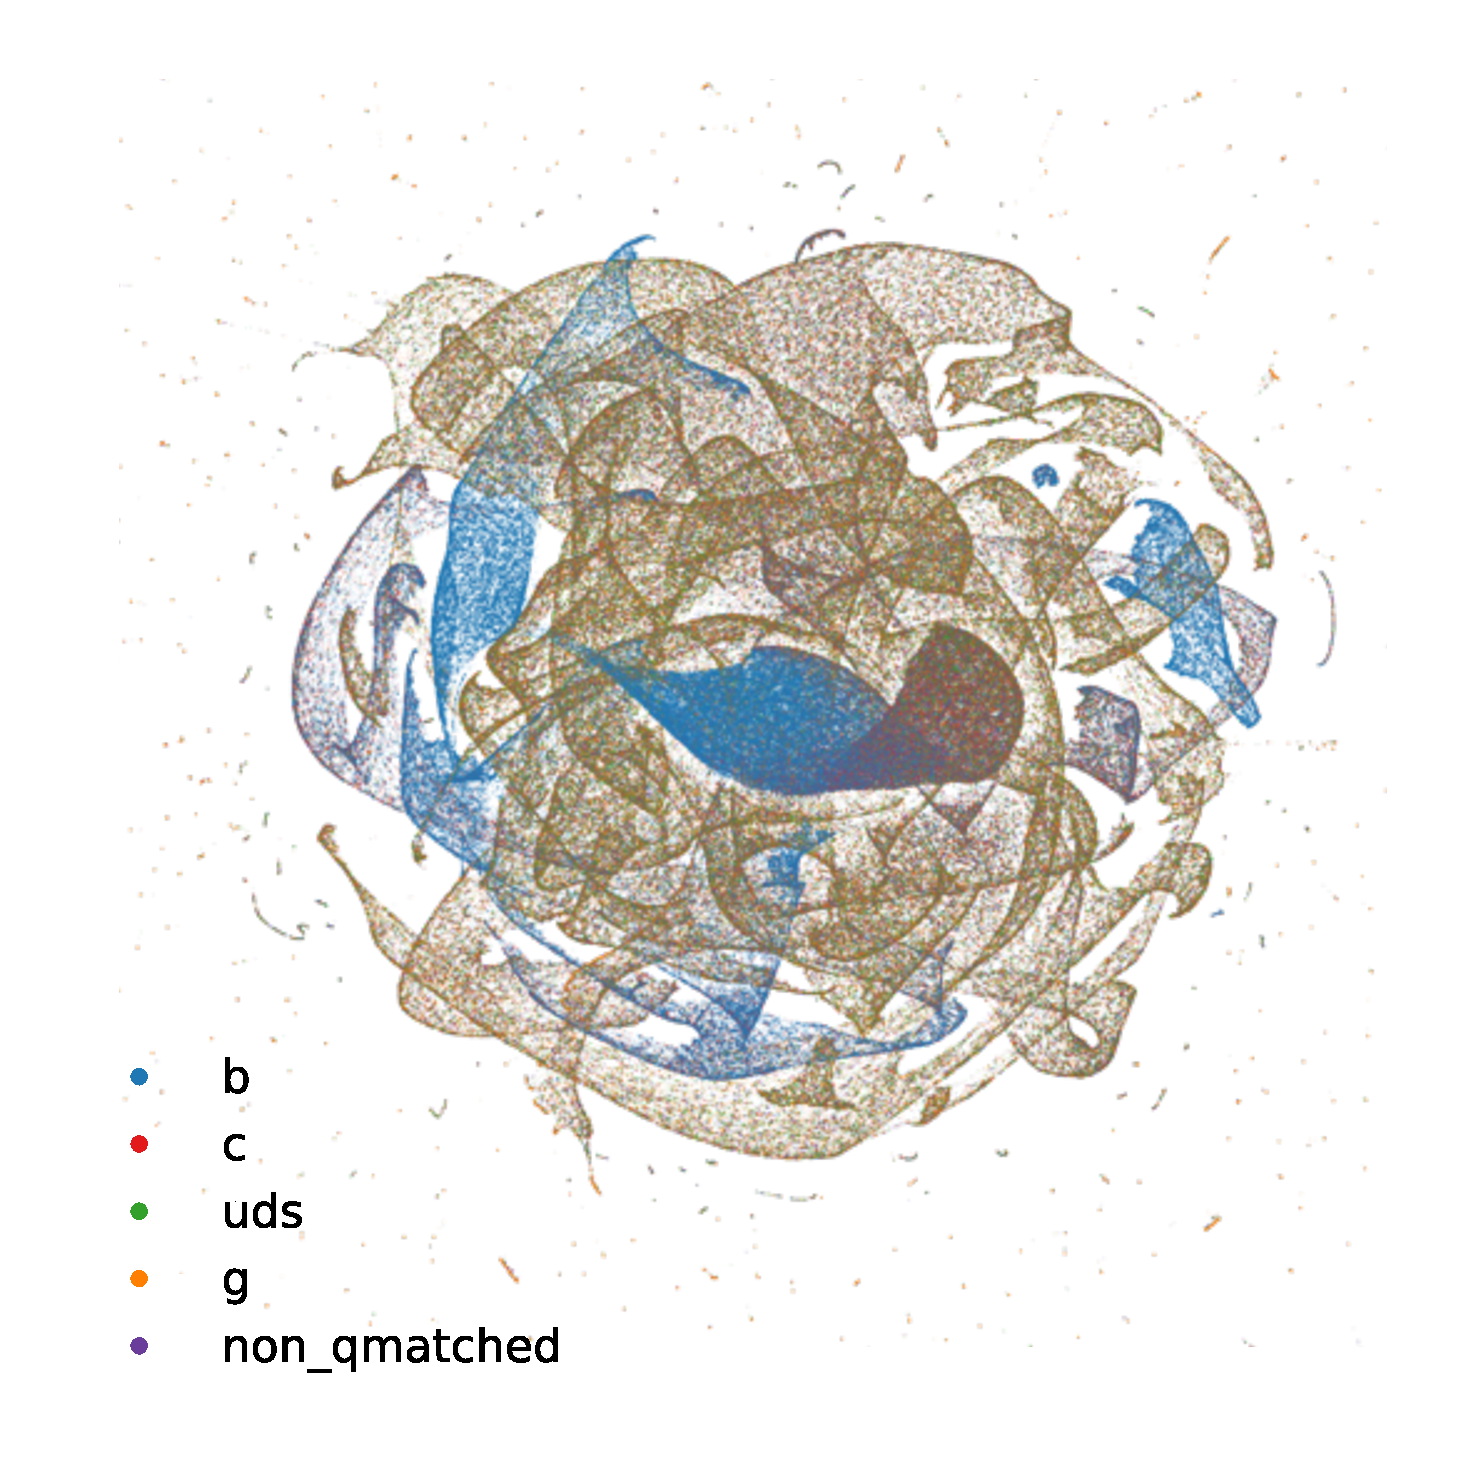
\includegraphics[draft=false, width=0.95\textwidth, trim=50 45 50 50, clip]{figures/quarks/df_UMAP-X=1078089-n_neighbors=250-min_dist=0.2-metric=euclidean-input2b_njet=3_algorithm=UMAP_single.pdf}
  \vspace{1mm}
  \caption[UMAP Visualization of the Vertex Variables for 3-Jet Events]
          {UMAP visualization of the vertex variables for 3-jet events.} 
  \label{fig:q:UMAP_vertex_3j}
\end{marginfigure}

% \begin{marginfigure}
%   \centerfloat
%   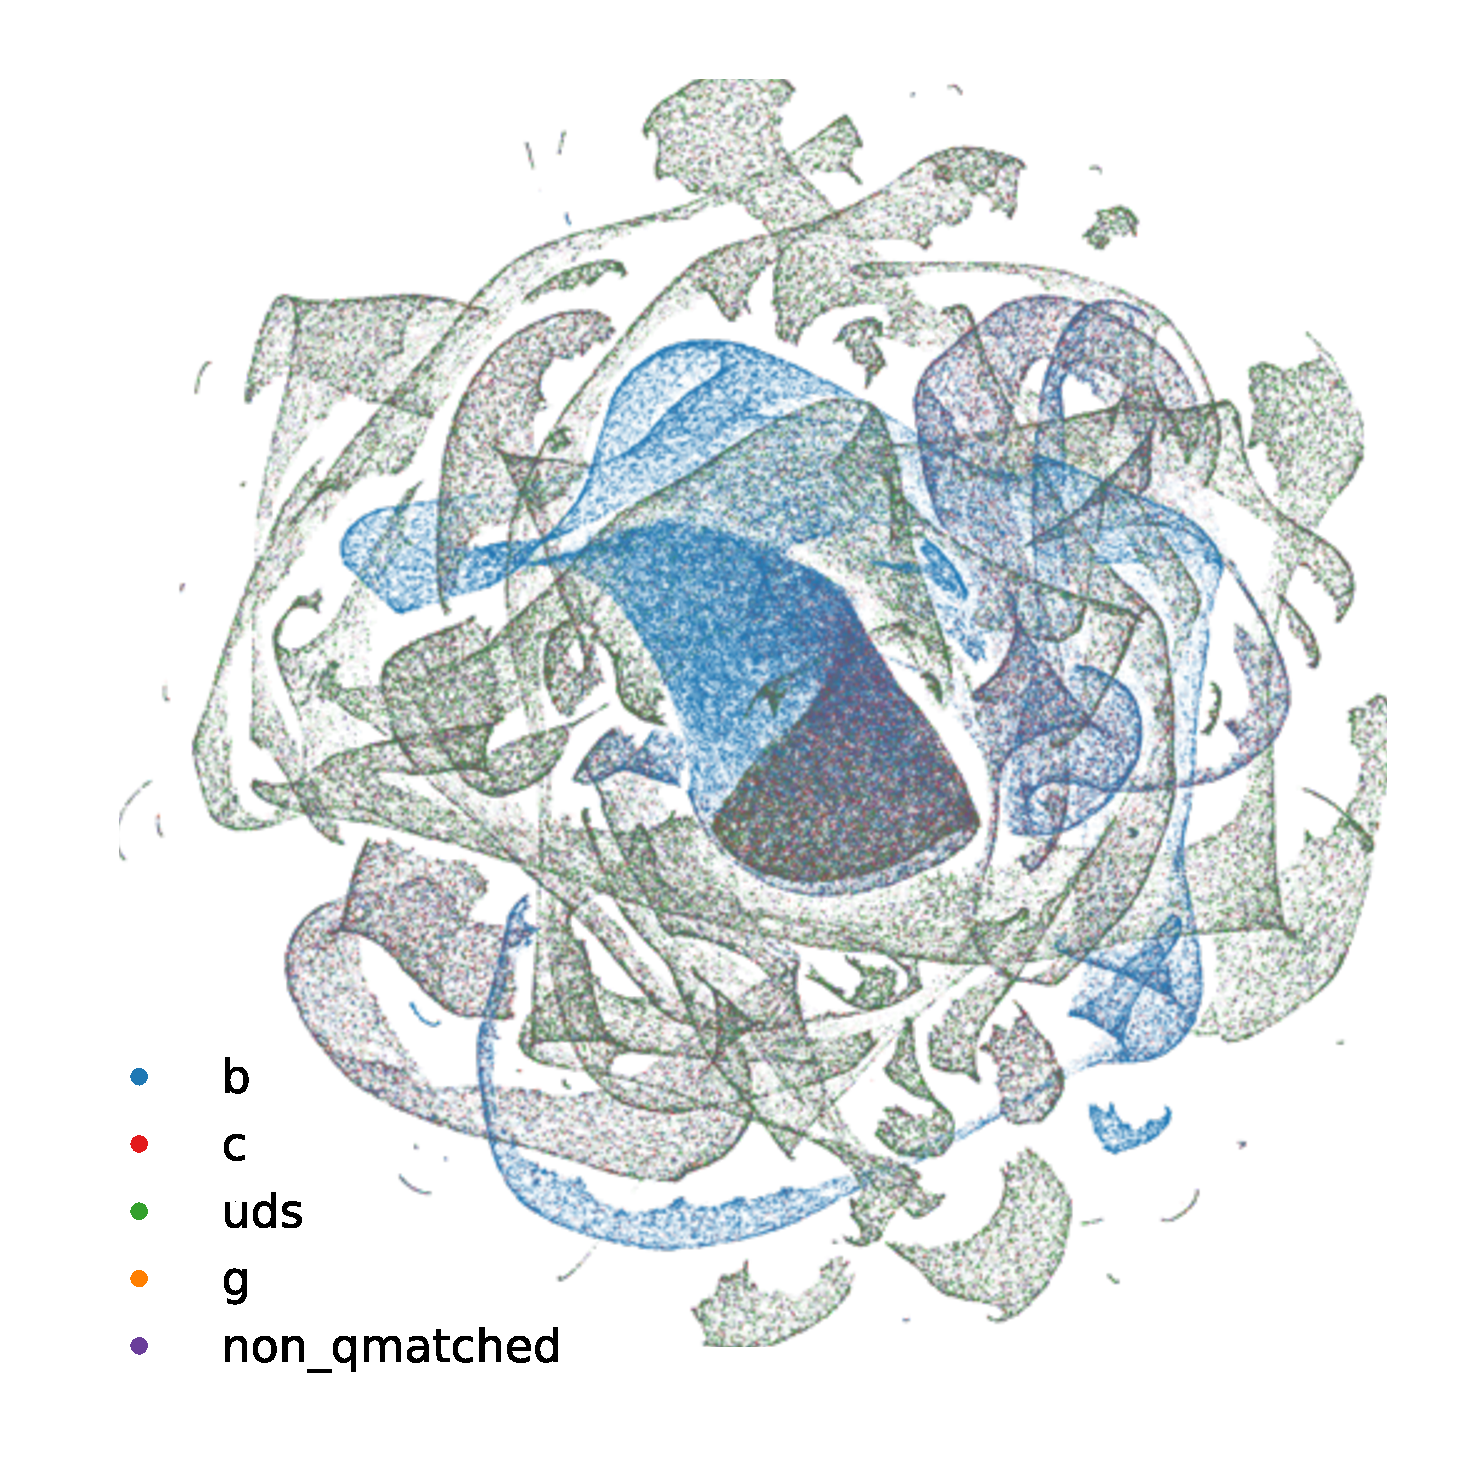
\includegraphics[draft=false, width=0.95\textwidth, trim=50 45 50 50, clip]{figures/quarks/df_UMAP-X=729358-n_neighbors=250-min_dist=0.2-metric=euclidean-input2b_njet=2_algorithm=UMAP_single.pdf}
%   \vspace{1mm}
%   \caption[UMAP Visualization of the Vertex Variables for 2-Jet Events]
%           {UMAP visualization of the vertex variables for 2-jet events.} 
%   \label{fig:q:UMAP_vertex_2j}
% \end{marginfigure}



\subsection{Correlations}

The correlations between the vertex variables are shown in Figure~\ref{fig:q:correlation_vertex_all}, where the upper diagonal shows the linear correlation $\rho$ and the lower diagonal shows the nonlinear correlation $\mathrm{MIC}_e$ introduced in \autoref{subsec:h:correlations_lin_mic}. It is found that \code{projet} and \code{bqvjet} have a relatively high correlation whereas the other variable combinations correlate much less. Had they all correlated a lot, it would be more difficult to extract any meaningful insights from the system as it would contain less information. 

\begin{figure}%
  \centering
  \subfloat[2-jet events]{{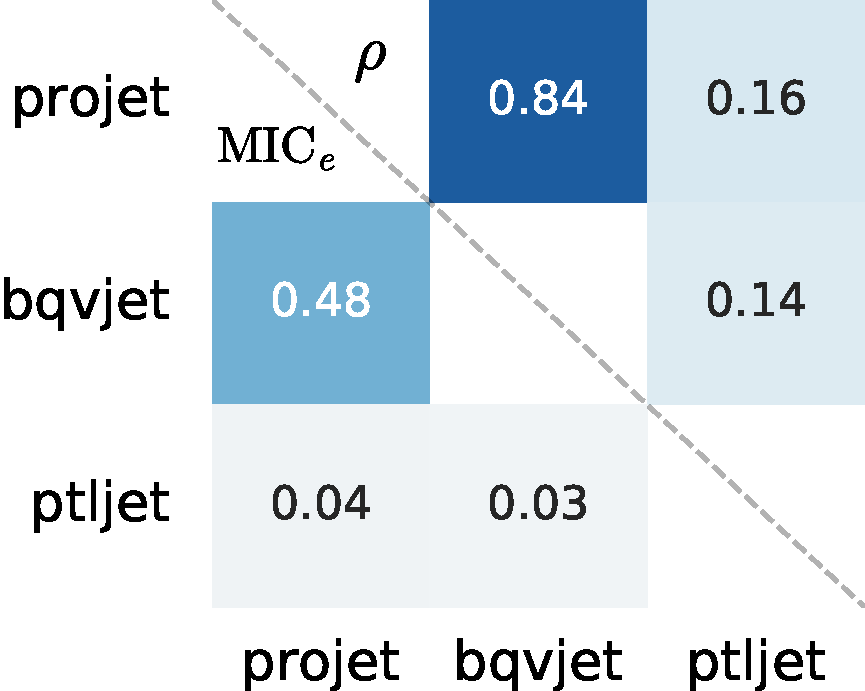
\includegraphics[height=3.15cm]{figures/quarks/correlations_vertex_vars-down_sample=1.00-ML_vars=vertex-selection=b-ejet_min=4-n_iter_RS_lgb=99-n_iter_RS_xgb=9-cdot_cut=0.90-version=19_njet=2.pdf} }}%
  \subfloat[3-jet events]{{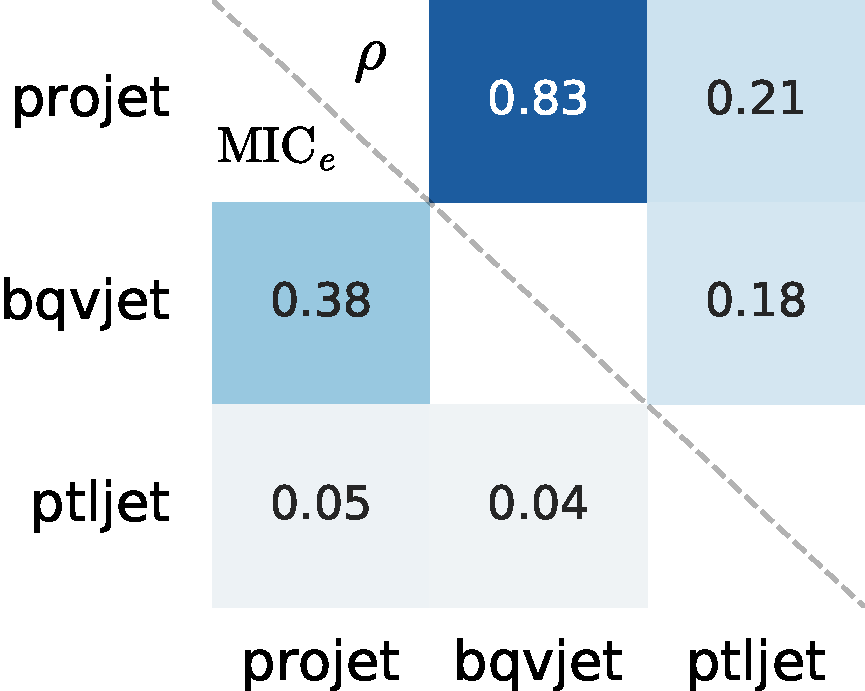
\includegraphics[height=3.15cm, trim=85 0 0 0, clip]{figures/quarks/correlations_vertex_vars-down_sample=1.00-ML_vars=vertex-selection=b-ejet_min=4-n_iter_RS_lgb=99-n_iter_RS_xgb=9-cdot_cut=0.90-version=19_njet=3.pdf} }}%
  \subfloat[4-jet events]{{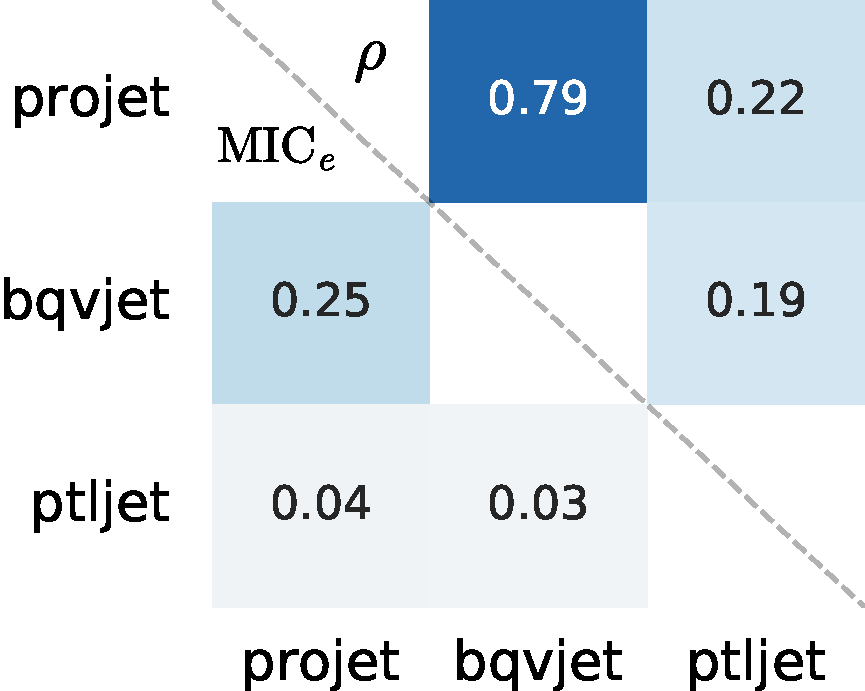
\includegraphics[height=3.15cm, trim=85 0 0 0, clip]{figures/quarks/correlations_vertex_vars-down_sample=1.00-ML_vars=vertex-selection=b-ejet_min=4-n_iter_RS_lgb=99-n_iter_RS_xgb=9-cdot_cut=0.90-version=19_njet=4.pdf} }}%
  \caption[Correlations Between of the Vertex Variables]{Correlations between the three vertex variables for 2-, 3- and 4-jet events. The upper diagonal shows the linear correlation $\rho$ and the lower diagonal the nonlinear correlations $\mathrm{MIC}_e$.}%
  \label{fig:q:correlation_vertex_all}%
\end{figure}

\FloatBarrier
\section{Loss and Evaluation Function}
\label{sec:q:loss_evaluation_function}

Contrary to the housing prices project where each house has a price on a continuous scale, the goal of the quark and gluon jet project is to predict types of jets or events where the \emph{signal} observations\sidenote[][-0.5cm]{Often called signal events, however, since a jet can also be signal, the term signal event is only used when the meaning is clear from the context.} are often assigned the label \num{1} and \emph{background} observations \num{0}. 
The combination of this being a \emph{classification} problem (compared to a regression problem). Furthermore, all the variables applied in the quark and gluon jet analysis are actual measurements from a particle detector which means that the issue of outliers is negligible.  This also means that the problem of finding a robust loss function is less important since for classification models the loss is already bounded in the $[0, 1]$\=/interval.

\emph{Accuracy}, which is simply the fraction of correct predictions, is often used as the loss function in classification, however, accuracy as a metric suffers a lot when handling \emph{imbalanced} data: when the ratio between the number of instances of each class is not approximately fifty-fifty. The problem is that if the sample contains \SI{90}{\percent} background and only \SI{10}{\percent} signal, then a simple model which simply predicts everything to be background will have a \SI{90}{\percent} accuracy.

To circumvent this issue, the area under the \emph{ROC}\sidenote{Receiver Operating Characteristic.} curve (\emph{AUC}) is used, where the ROC curve is the the \emph{signal efficiency} $\varepsilon_\mathrm{sig}$ of the ML model plotted as a function\marginnote{Strictly speaking it is not a function of the background efficiency, but rather $\varepsilon_\mathrm{sig}$ and $\varepsilon_\mathrm{bkg}$ plotted parametrically as functions of the threshold cut $\hat{y}_\mathrm{cut}$.} of the \emph{background efficiency} $\varepsilon_\mathrm{bkg}$. The definition of these two measures are:
\begin{equation}
  \varepsilon_\mathrm{sig} = \frac{S_\mathrm{sel}}{S_\mathrm{tot}}\,, \qquad \varepsilon_\mathrm{bkg} = \frac{B_\mathrm{sel}}{B_\mathrm{tot}}\,,
\end{equation}
where $S_\mathrm{sel}$ are signal events that were also selected (predicted) as signal by the ML model, $S_\mathrm{tot}=S_\mathrm{sel}+S_\mathrm{rej}$ is the total number of signal events (the selected and rejected), and likewise for background events $B$. Within the machine learning community the signal efficiency is called the true positive rate (TPR) and the background efficiency the false positive rate (FPR). For the rest of this project, the AUC will be the evaluation function $f_\mathrm{eval} = \mathrm{AUC}$, however, since this metric does not work on single observations it cannot be used as the loss function. Instead we will use the \emph{log-loss} as the loss function\sidenote{In the context of machine learning this is the same as the \emph{cross entropy}.} which in comparison to the AUC is not only differentiable for single predictions but also takes the certainty of the prediction into account. When using tree-based algorithms or neural networks one can compute not only whether or not a single observation is classified as signal or background but also a prediction score. This is a number in the $[0, 1]$\=/interval and the closer to \num{1} the score is, the more certain the model is of the prediction being signal. Given the prediction score $\hat{y}$ and the true label $y$, the log-loss $\ell_\mathrm{log}$ is calculated as:
\begin{equation}
    \ell_\mathrm{log}(\hat{y}, y) = -y \log{\hat{y}} - (1-y) \log{(1-\hat{y})}.
\end{equation}
This is visualized in Figure~\ref{fig:q:logloss}. Here it can be seen how the loss changes as a function of the prediction score. Notice that when $y=0$ the loss for $\hat{y}=1$ diverges towards $\infty$ and likewise with $y=1$ and $\hat{y}=0$ (since $\log 0$ diverges to $\=/\infty$).

\begin{marginfigure}[-5cm]
  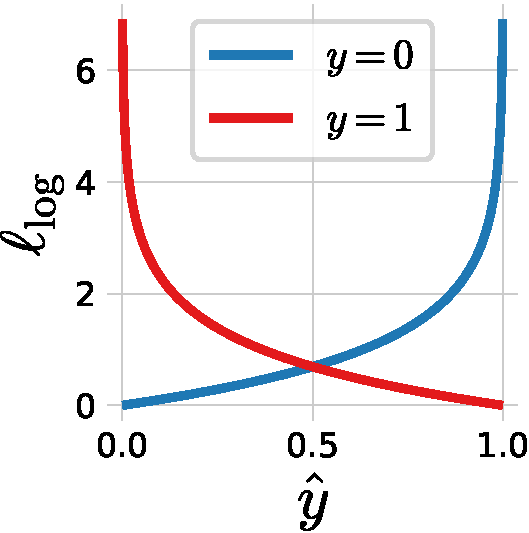
\includegraphics[draft=false, width=0.9\textwidth]{figures/log_loss_cross_entropy/logloss.pdf}
  \caption[Plot of the Log-Loss $\ell_\mathrm{log}$]
          {Plot of the log-loss $\ell_\mathrm{log}$ for \textcolor{blue}{background ($y=0$)} in blue and \textcolor{red}{signal ($y=1$)} in red.} 
  \label{fig:q:logloss}
\end{marginfigure}

\FloatBarrier
\section[b-Tagging Analysis]{$b$\=/Tagging Analysis}
\label{sec:q:b_tagging_analysis}

The ability to discriminate between the different types of particles produced in a collision is obviously important in order to correctly interpret the measurements. A lot of research focus on tagging algorithms today, e.g. $b$\=/tagging in ATLAS and CMS \autocite{scodellaroTaggingATLASCMS2017}. The reason that $b$\=/quarks are tagged specifically is both due to $b$\=/quarks having more unique characteristics compared to e.g. $c$\=/quarks and are thus easier to tag, but also the fact that $b$\=/quarks are the second-heaviest of the quarks and are measured to better understand CP-violation\sidenote{Short for charge-parity.} at LHC-b, contributes to the choice of tagging $b$\=/quarks. In ALEPH \citet{proriolTAGGINGQUARKEVENTS1991} started the work of comparing different methods for $b$\=/tagging already in \num{1991}. They concluded that a neural network had the best performance compared to e.g. a linear (Fisher) discriminant. The neural network used was a 3-layer neural network (NN) trained on nine variables for which the output was the predicted score \code{nnbjet}. From here on, this pre-trained network will be called NNB. The events are split in a $(80 \dash 20)\si{\percent}$ train-test ratio in such a way that the individual jets in an event are not split. 

\subsection{$b$\=/Tagging Hyperparameter Optimization}

Compared to the housing prices dataset, the number of observations $N$ has significantly increased ($\num{3e7} \gg \num{5e5}$), but the dimensionality $M$ is much smaller ($3 \ll 143 $). Therefore both XGBoost (XGB) and LightGBM (LGB) were included as models initially since their performances in the housing dataset were very similar. LightGBM was expected to be faster on this dataset due to the large $N$. The models were hyperparameter optimized (HPO) using random search (RS) since the Bayesian optimization (BO) did not show any performance gains compared to RS in the housing project. 

\begin{margintable}[-2cm]
  \centerfloat
  % \vspace{3mm}
  \begin{tabular}{@{}ll@{}}
  Hyperparameter          &  Range                                  \\ \midrule
  \code{subsample}        & $\mathcal{U}(0.4, 1)$                   \\
  \code{colsample_bytree} & $\mathcal{U}_\mathrm{trunc}(0.4, 1, 2)$ \\
  \code{max_depth}        & $\mathcal{U}_\mathrm{int}(-5, 63)$      \\
  \code{num_leaves}       & $\mathcal{U}_\mathrm{int}(7, 4095)$     \\
  \end{tabular}
  % \vspace{\abovecaptionskip}
  \vspace{3mm}
  \caption[Random Search PDFs for LGB]{\label{tab:q:hpo_ranges_lgb}Probability Density Functions for the random search hyperparameter optimization process for the LightGBM model. For an explanation of $\mathcal{U}_\mathrm{trunc}$, see \autoref{subsec:q:trunc_uniform}. All negative values of \code{max_depth} are interpreted as no max depth by both LGB and XGB.}
\end{margintable}

They were both hyperparameter optimized with $5$\=/fold cross validation and early stopping with a patience of \num{100}. The PDFs for the random search for the LightGBM model can be seen in Table~\ref{tab:q:hpo_ranges_lgb}, and the ones for XGBoost in Table~\ref{tab:q:hpo_ranges_xgb}. The random search has been run with \num{100} iterations for LightGBM and only \num{10} iterations for XGBoost since XGBoost turned out to be very slow\sidenote{See page \pageref{page:q:timings_b_tag} for a discussion of the timings.} at fitting datasets of this size. 

\begin{figure*}%
  \centerfloat
  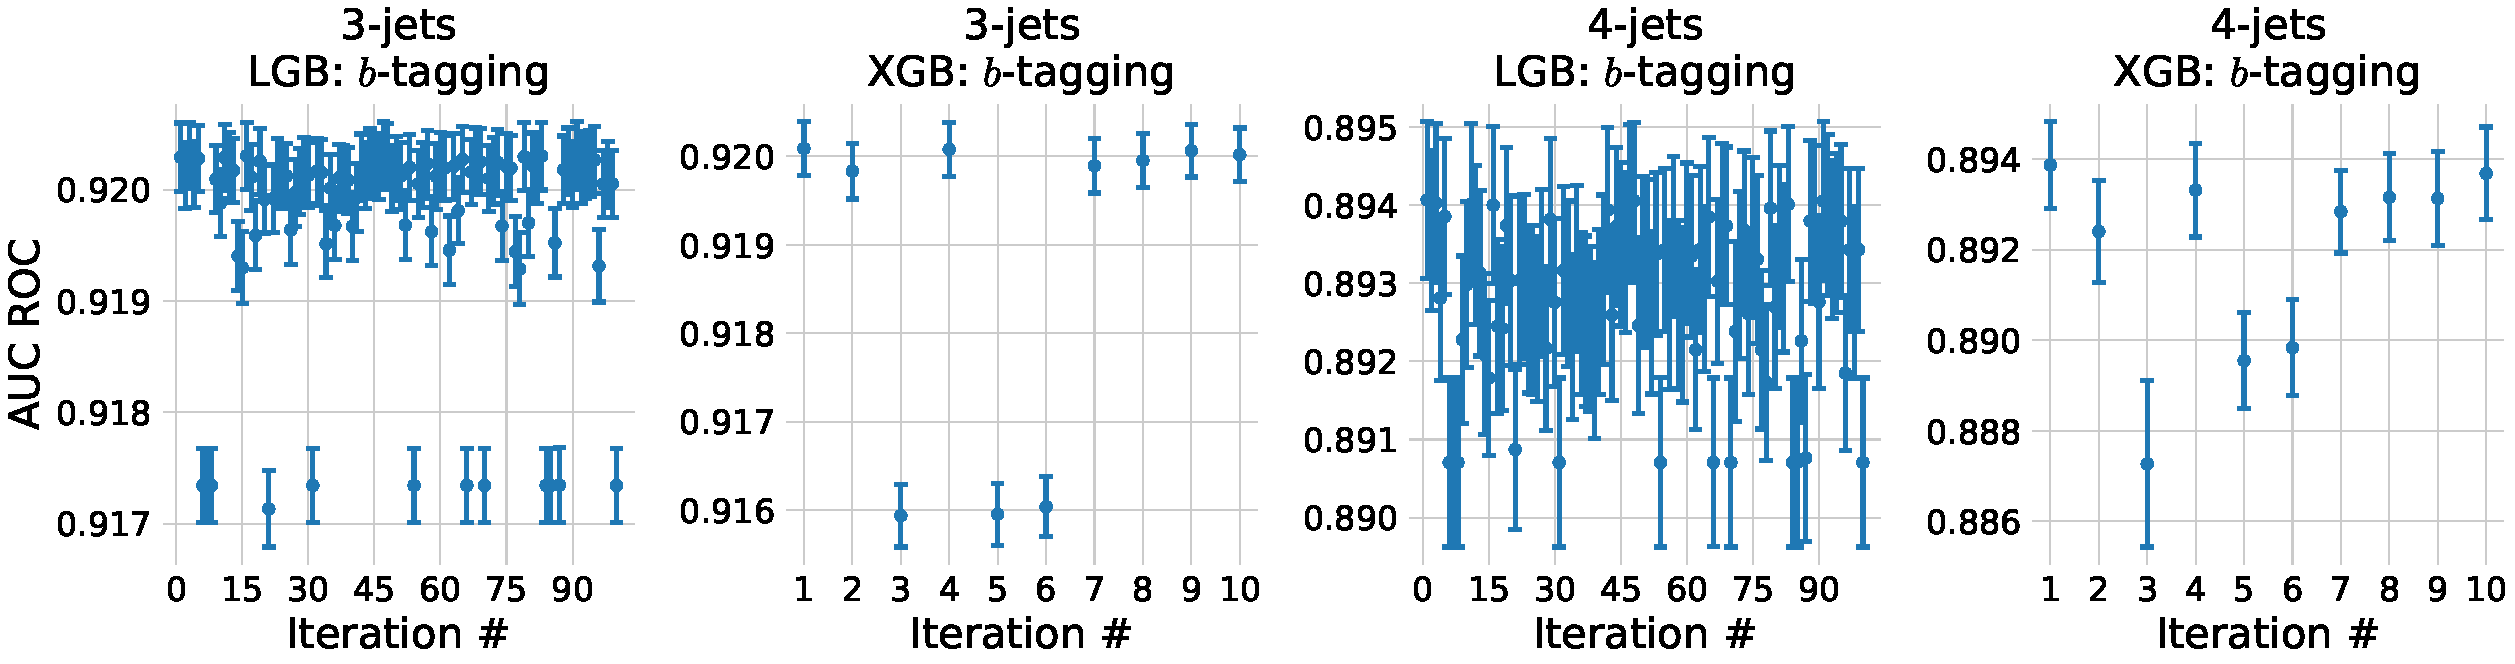
\includegraphics[width=\textwidth, trim=0 0 0 0, clip]{figures/quarks/cv_res_lgb-btag-down_sample=1.00-ML_vars=vertex-selection=b-ejet_min=4-n_iter_RS_lgb=99-n_iter_RS_xgb=9-cdot_cut=0.90-version=19.pdf}
  \vspace{3mm}
  \caption[Hyperparameter Optimization of $b$\=/Tagging]{
    Hyperparameter Optimization results of $b$\=/tagging with random search. From left to right, we have A) \num{100} iterations of RS with LGB on 3-jets, B) \num{10} iterations of RS with XGB on 3-jets, C) \num{100} iterations of RS with LGB on 4-jets, D) \num{10} iterations of RS with XGB on 4-jets. }
  \label{fig:q:CV_res_iterations_b_tagging}%
\end{figure*}
\vspace{-3mm}

The results of the HPO for 3-jet and 4-jet events can be seen in Figure~\ref{fig:q:CV_res_iterations_b_tagging}. For 3-jets it can be seen how most of the iterations share about the same performance (within $1\sigma$), however, some iterations show a significant decrease in performance. The same clear pattern is not found in the 4-jet events.

The relationship between the different hyperparameters in 4-jet events can be seen in the parallel coordinate plot in Figure~\ref{fig:q:initial_CV_res_parallel_coords_4j}. First of all the importance of the column downsampling \code{colsample_bytree} variable is significant: all of the low-performing hyperparameter sets have a low value of this hyperparameter. Since $M=3$ for the vertex variables this makes logical sense; using only $\mathrm{int}(\sim 0.5 \cdot 3) = 1$ variable\sidenote{See \autoref{subsec:q:trunc_uniform} for a deeper discussion about the \code{colsample_bytree} hyperparameter.} the model cannot properly learn the structure in the data. Compared to the column downsampling, the other hyperparameters are less important. The same overall conclusion can be inferred in the 3-jet case, see Figure~\ref{fig:q:initial_CV_res_parallel_coords_3j}.

\begin{figure}
  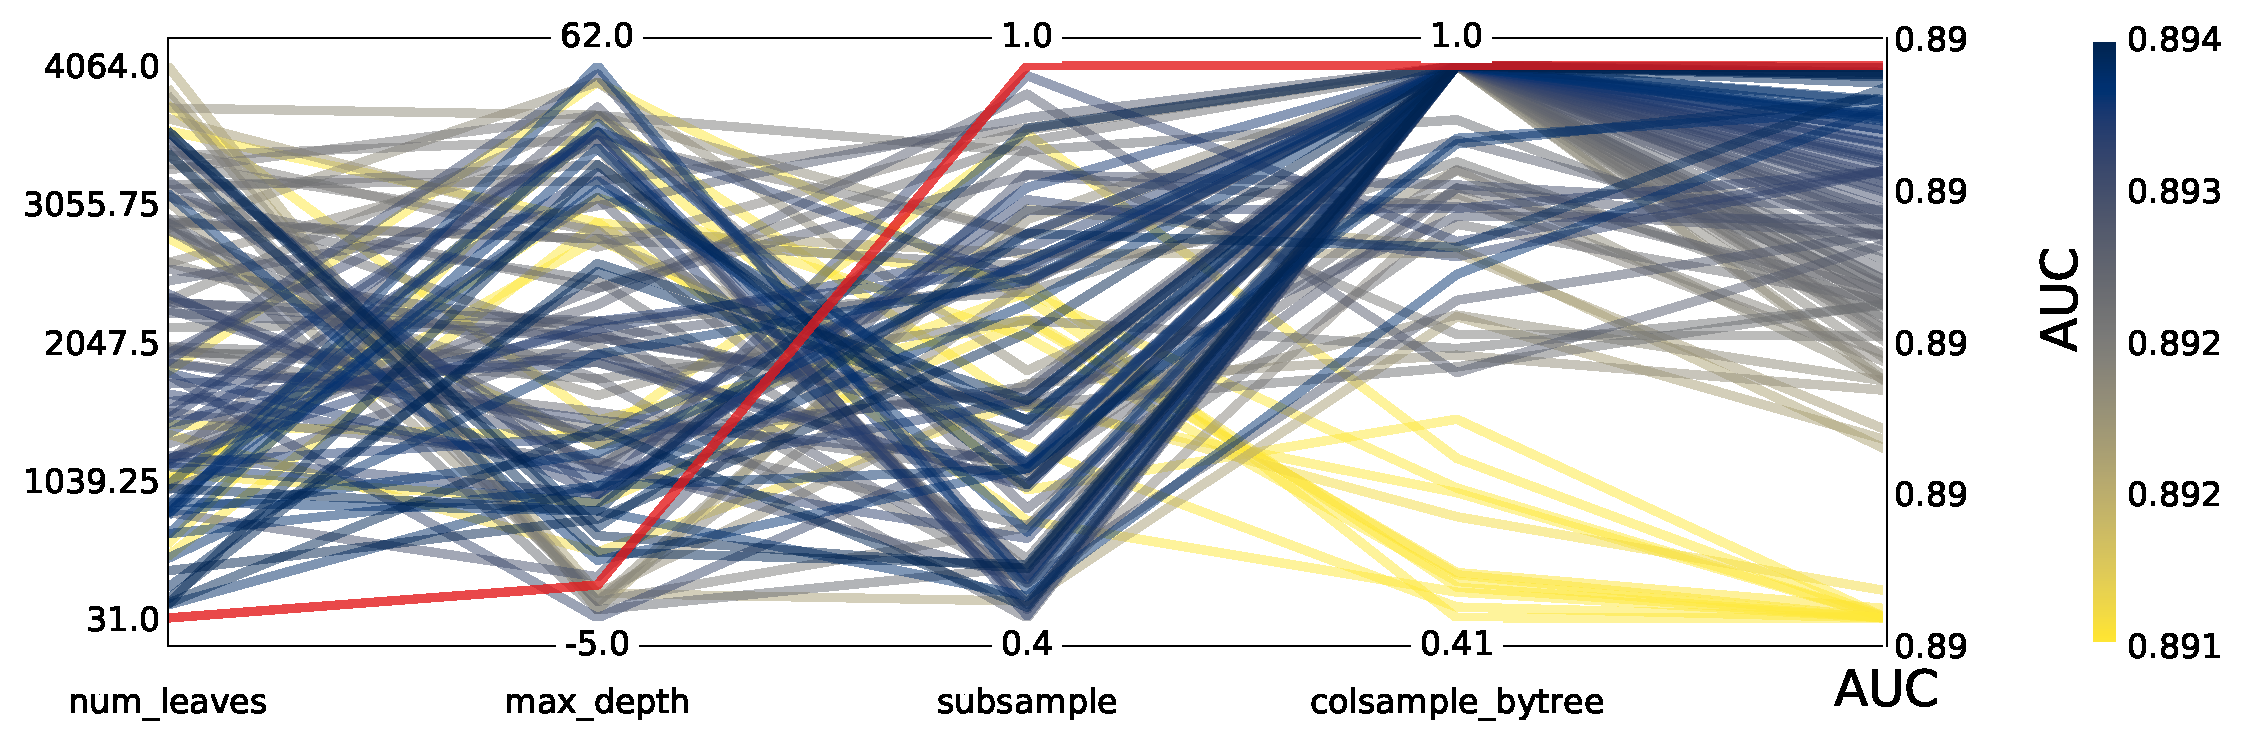
\includegraphics[width=0.98\textwidth, trim=0 0 0 0, clip]{figures/quarks/CV_viz-njet=4-name=lf_lgb_down_sample=1.00-ML_vars=vertex-selection=b-ejet_min=4-n_iter_RS_lgb=99-n_iter_RS_xgb=9-cdot_cut=0.90-version=19.pdf}
  \caption[Parallel Plot of HPO Results for 4-Jet $b$\=/Tagging]
          {Hyperparameter optimization results of $b$\=/tagging for 4-jet events. The results are shown as parallel coordinates with each hyperparameter along the $x$\=/axis and the value of that parameter on the $y$\=/axis. Each line is an event in the 4-dimensional space colored according to the performance of that hyperparameter as measured by AUC. The \textcolor{red}{single best hyperparameter} is shown in red. 
          } 
  \label{fig:q:initial_CV_res_parallel_coords_4j}
\end{figure}

\subsection{$b$\=/Tagging Results}

The prediction score $\hat{y}$ is usually called the $b$\=/tag for $b$\=/tagging models and will be written as $\beta_\mathrm{tag}$. The distribution of the $b$-tags for the two HPO-optimized models, LGB and XGB, together with the pre-trained neural network, NNB, can be seen in Figure~\ref{fig:q:btag_scores_4j} for 4-jet events and in \ref{fig:q:btag_scores_3j} for 3-jet events. Notice the strong match between the NNB and LGB models. The XGB model has almost no high $b$\=/tags ($\beta_\mathrm{tag} > 0.8$), but a majority of $b$\=/tags in the very low end. This indicates that the XGBoost has focussed on the background events compared to the signal events, whereas the NNB and LGB models have focused more on the signal events. 

\begin{figure}[h!]
  \vspace{-0.3cm}
  \centerfloat
  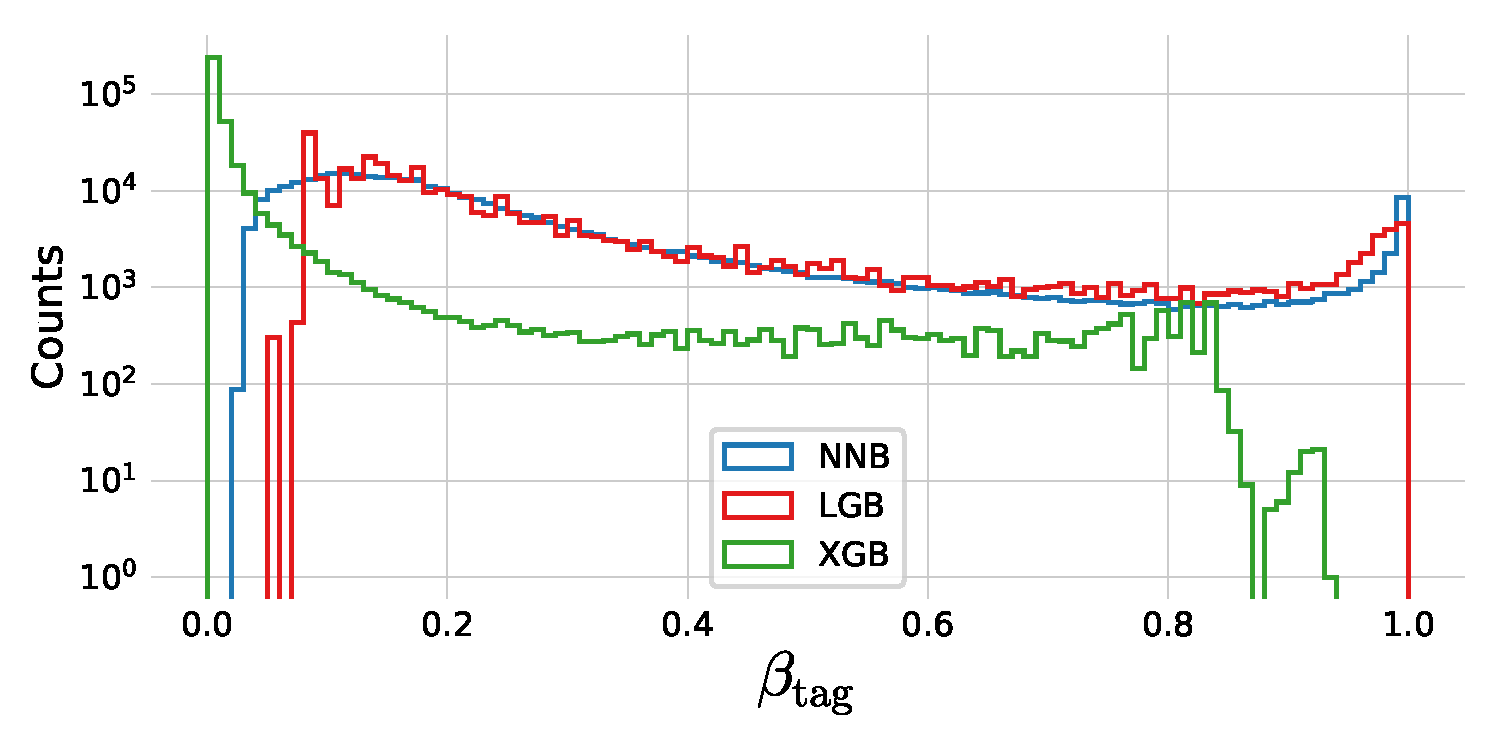
\includegraphics[width=0.95\textwidth, trim=5 15 10 10, clip]{figures/quarks/y_pred_4_jet_hist-down_sample=1.00-ML_vars=vertex-selection=b-ejet_min=4-n_iter_RS_lgb=99-n_iter_RS_xgb=9-cdot_cut=0.90-version=19.pdf}
  \caption[$b$\=/Tag Scores in 4-Jet Events]
          {Histogram of $b$\=/tag scores $\beta_\mathrm{tag}$ in 4-jet events for \textcolor{blue}{NNB} (the neural network pre-trained by ALEPH, also called \code{nnbjet}) in blue, \textcolor{red}{LGB} in red, and \textcolor{green}{XGB} in green. 
          } 
  \label{fig:q:btag_scores_4j}
\end{figure}
\vspace{-0.3cm}

Even though the distributions of $b$\=/tags are different between the three models, the real performance plot for classification is the ROC curve seen in Figure~\ref{fig:q:roc_btag_4j} for 4-jet events. Here the signal efficiency $\varepsilon_\mathrm{sig}$ is plotted as a function of the background efficiency $\varepsilon_\mathrm{sig}$ with the AUC shown in the bottom right corner. The LGB and XGB models performs similarly well with an $\mathrm{AUC}=0.896$ compared to the NNB with $\mathrm{AUC}=0.884$. The differences between the models are even smaller for 3-jet events seen in Figure~\ref{fig:q:roc_btag_3j}. In general the LGB and XGB models are so similar that they cannot be distinguished from another in any of the plots and their difference in AUC is on the fourth decimal point. \label{page:q:timings_b_tag}

\begin{figure}[h!]
  \vspace{-0.1cm}
  \centerfloat
  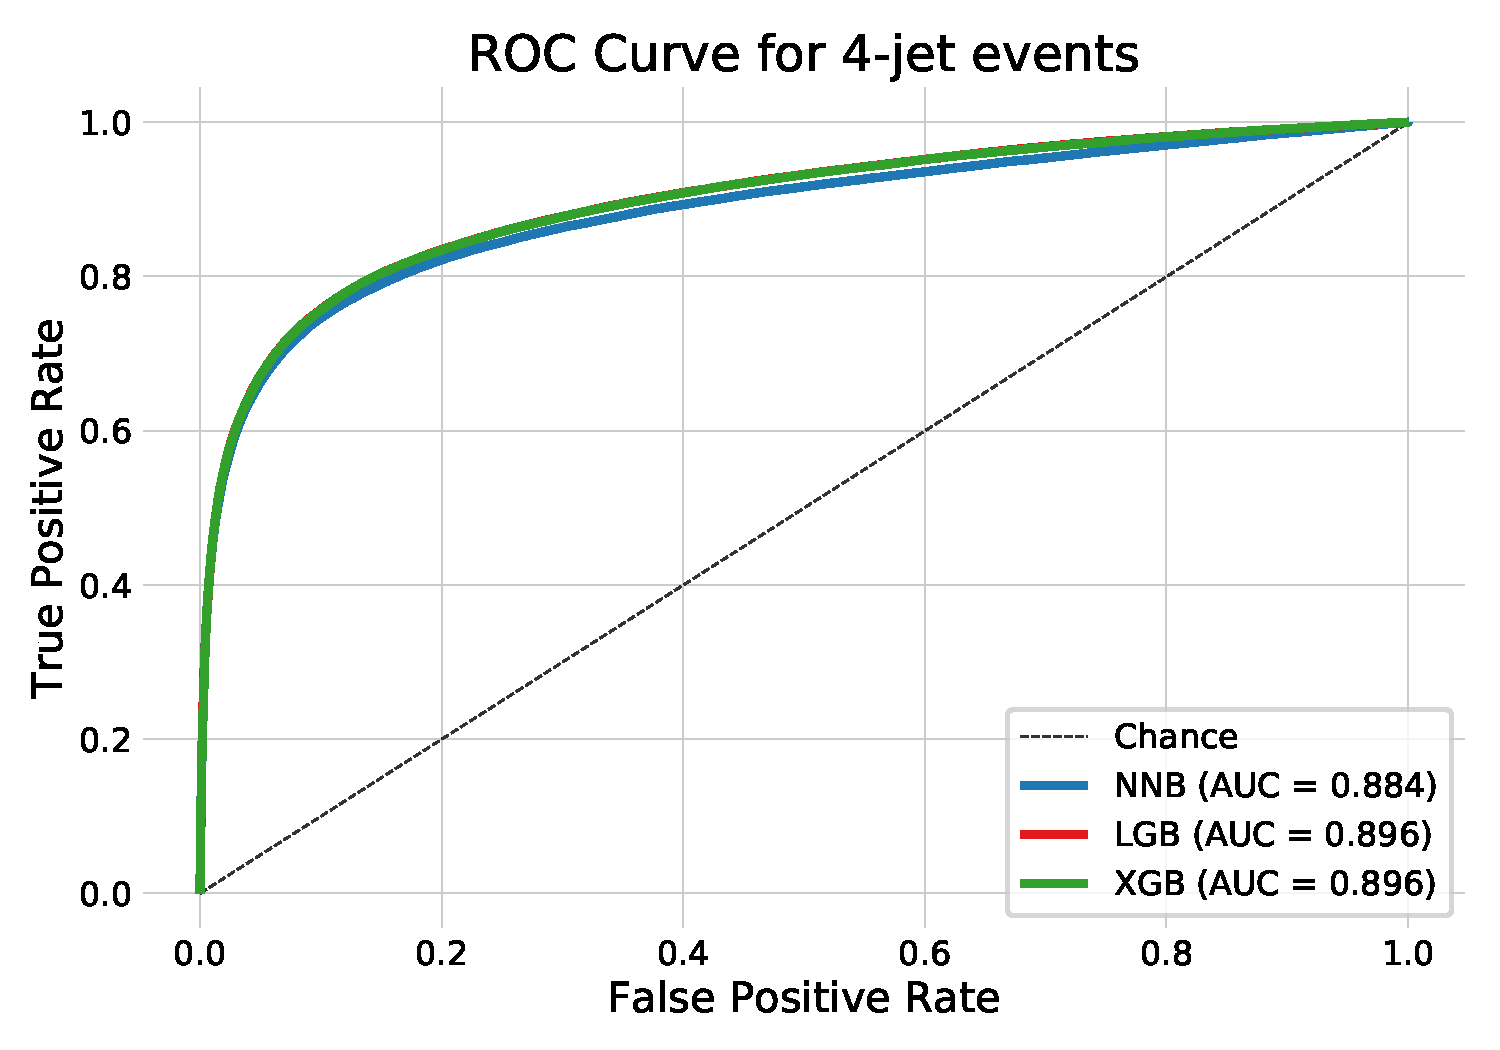
\includegraphics[width=0.99\textwidth, trim=10 10 10 40, clip]{figures/quarks/ROC_4_jet-down_sample=1.00-ML_vars=vertex-selection=b-ejet_min=4-n_iter_RS_lgb=99-n_iter_RS_xgb=9-cdot_cut=0.90-version=19.pdf}
  \caption[ROC Curve for 4-Jet $b$\=/Tagging]
          {ROC curve of the three $b$\=/tag models in 4-jet events for \textcolor{blue}{NNB} (the pre-trained neural network trained by ALEPH, also called \code{nnbjet}) in blue, \textcolor{red}{LGB} in red, and \textcolor{green}{XGB} in green. In the legend the area under curve (AUC) is also shown. Notice that the LGB and XGB models share performance and it is thus due to overplotting that only the green line for XGB can be seen. 
          } 
  \label{fig:q:roc_btag_4j}
\end{figure}
\vspace{-0.3cm}

The LGB model is, however, several times faster than the XGB model. In comparison, \num{10} iterations of HPO using RS on 3-jet events with XGB took more almost \num{34} hours on HEP\sidenote{The local computing cluster.} compared to just \num{23} hours for \num{100} iterations for LGB. The same performance difference was seen in 4-jet events where the timings were \num{4} hours for XGB compared to \num{2.5} hours for LGB. Since their performance is similar, XGB is dropped in the subsequent analysis. 

The distribution of the $b$\=/tag scores $\beta_\mathrm{tag}$ for signal and background in 4-jet events can be seen in Figure~\ref{fig:q:btag_histogram_4j}. The separation between the heavier quarks and light quarks (and gluons) is clear at high values of $\beta_\mathrm{tag}$, however, a lot of $c$\=/quarks also get a high $b$\=/tag score. The same is seen for 3-jet events in Figure~\ref{fig:q:btag_histogram_3j}. 

\vspace{-5mm}
\begin{figure}[h!]
  \centerfloat
  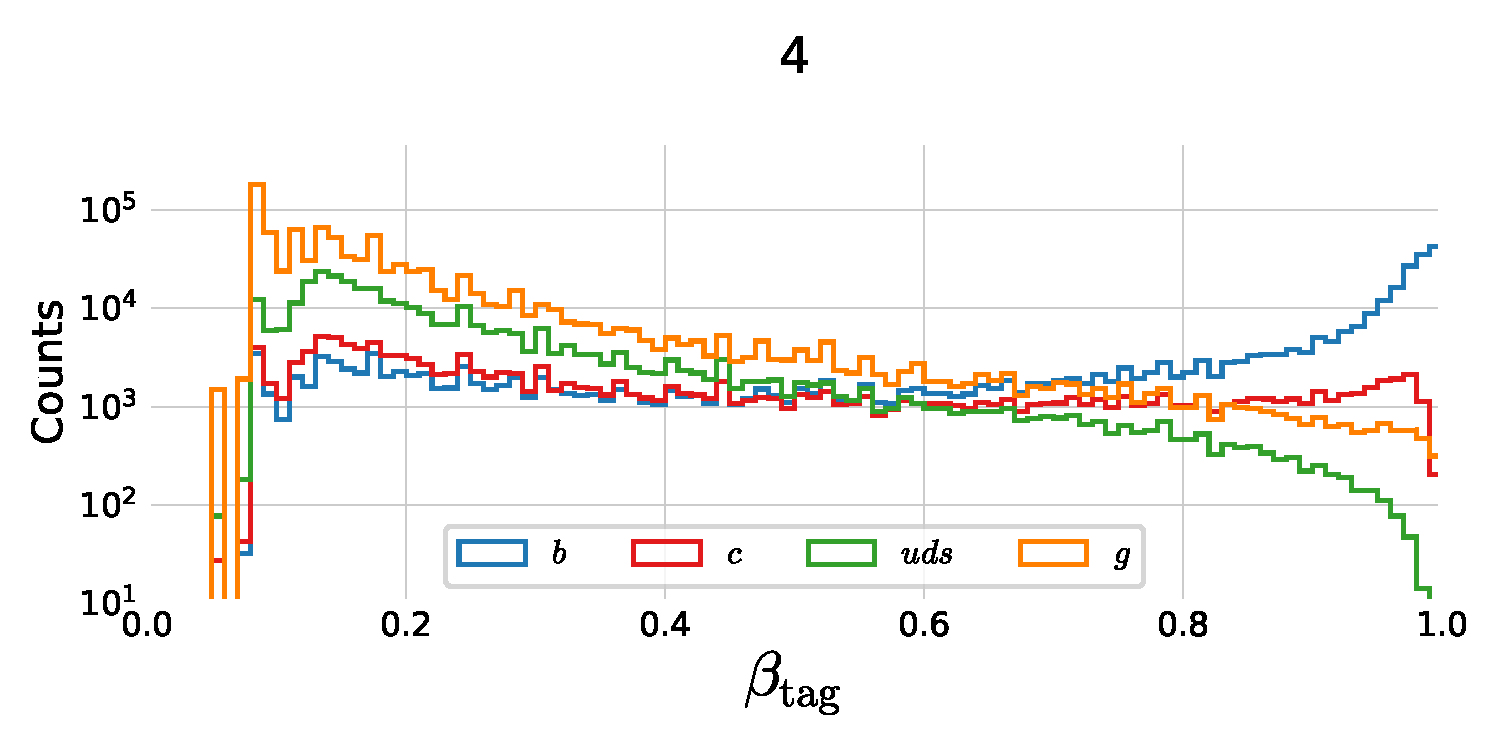
\includegraphics[width=0.95\textwidth, trim=15 15 15 50, clip]{figures/quarks/btag_scores_histogram_-njet=4-down_sample=1.00-ML_vars=vertex-selection=b-ejet_min=4-n_iter_RS_lgb=99-n_iter_RS_xgb=9-cdot_cut=0.90-version=19.pdf}
  \vspace{2mm}
  \caption[Distribution of $b$\=/Tags in 4-Jet Events]
          {Distribution of $b$\=/tags in 4-jet events for \textcolor{blue}{$b$\=/jets} in blue, \textcolor{red}{$c$\=/jets} in red, \textcolor{green}{$uds$} in green and \textcolor{orange}{$g$} in orange.} 
  \label{fig:q:btag_histogram_4j}
\end{figure}
\vspace{-5mm}

\subsection{$b$\=/Tagging Model Inspection}

To get a better understanding of the trained LGB model, the global SHAP feature importances are shown in Figure~\ref{fig:q:shap_btag_global_4j} for 4-jet events. First of all it is noted that the \code{projet} has global feature importance of \SI{57.32}{\percent}, \code{bqvjet} \SI{29.16}{\percent}, and \code{ptljet} \SI{13.52}{\percent}. For all three variables it is seen how most of the points have many small feature values which has a (small) negative impact on the model output. Especially the \code{ptljet} has many features with a low value (\num{0} in fact) yet this does not pull the model too much towards background events. Compared this to a jet with a high value of \code{ptljet} which has a strong, positive impact on the output prediction.

\begin{figure}[h!]
  \centerfloat
  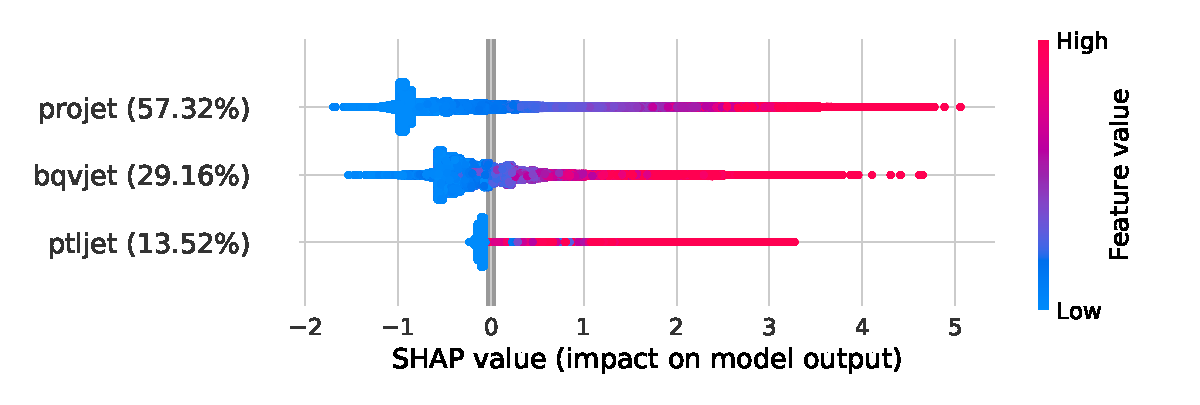
\includegraphics[width=0.98\textwidth, trim=10 10 20 10, clip]{figures/quarks/shap_global-down_sample=1.00-ML_vars=vertex-selection=b-ejet_min=4-n_iter_RS_lgb=99-n_iter_RS_xgb=9-cdot_cut=0.90-version=19-njet=4.pdf}
  \caption[Global Feature Importances for the LGB $b$\=/Tagging Algorithm on 4-Jet Events]
          {Global feature importances for the LGB $b$\=/tagging algorithm on 4-jet events. The normalized feature importance is shown in the parenthesis and the each dot is an observation showing the dependance between the SHAP value and the feature value. 
          } 
  \label{fig:q:shap_btag_global_4j}
\end{figure}



In regression, the model output is a continuous prediction ${\hat{y}_\mathrm{reg} \in \mathbb{R}}$. In classification what is actually happening under the hood is that the model predicts a value $\tilde{y} \in \mathbb{R}$ which is transformed to a number in the $[0, 1]$\=/interval via the \emph{expit} function:
\begin{equation}
    \label{eq:q:expit}
    \mathrm{expit(\tilde{y})} = \frac{e^{\tilde{y}}}{1+e^{\tilde{y}}} \equiv p,
\end{equation}

\begin{marginfigure}[-2.5cm]
  \centerfloat
  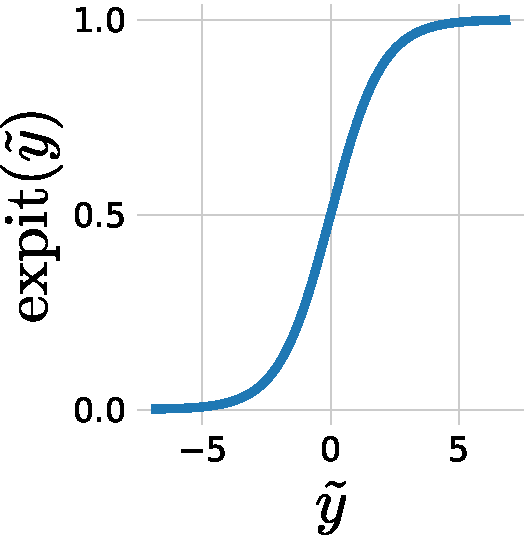
\includegraphics[width=0.8\textwidth]{figures/logit_expit/expit.pdf}
  \caption[The Expit Function]
          {The expit function.} 
  \label{fig:q:expit}
\end{marginfigure}

\noindent where $p$ is a number in the $[0, 1]$\=/interval. The expit function is also sometimes known as the logistic function and is visualized in Figure~\ref{fig:q:expit}. Its inverse is the \emph{logit} function:
\begin{equation}
  \label{eq:q:logit}
  \mathrm{logit}(p) = \log \left( \frac{p}{1-p}  \right) = \tilde{y},
\end{equation}

 \begin{marginfigure}
  \centerfloat
  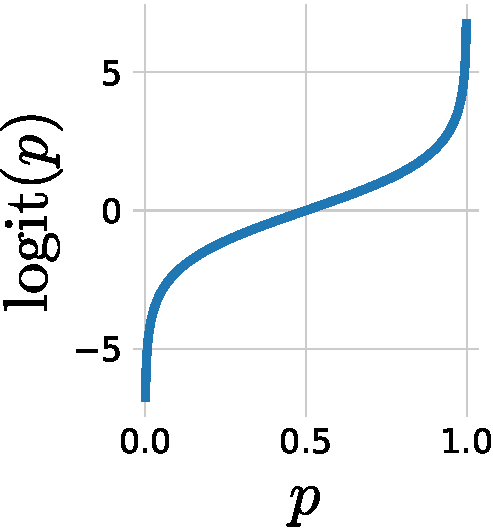
\includegraphics[width=0.8\textwidth]{figures/logit_expit/logit.pdf}
  \caption[The Logit Function]
          {The logit function.} 
  \label{fig:q:logit}
\end{marginfigure}

 \noindent which is visualized in Figure~\ref{fig:q:logit}. The fraction in equation \eqref{eq:q:logit} is called the \emph{odds} and the logit-transformed value of $p$, $\mathrm{logit}(p)=\tilde{y}$, is thus sometimes called the \emph{log-odds}. Because LightGBM makes its predictions in this log-odds space, the SHAP values in Figure~\ref{fig:q:shap_btag_global_4j} are also in log-odds space\sidenote[][5mm]{The additivity property of SHAP, see \autoref{sec:ml:feature_importance}, is thus also in this log-odds space.}. 

With this in mind, single predictions of the LGB $b$\=/tagging model can be understood with SHAP which Figure~\ref{fig:q:shap_single_prediction_3j} is an example of. This plot, which is my own extension to Figure~\ref{fig:h:shap_single_apartment}, shows the logic behind the model's prediction for a particular jet in a particular 3-jet event. That the bias is negative reflects that there is a majority of background jets compared to signal jets\sidenote{Only around \SI{22}{\percent} of all the jets are $b$\=/jets.}. This particular event has \code{projet}$=1.003$, \code{bqvjet}$=0.529$, and \code{ptljet}$=0$. In the plot it is seen how this high value of \code{projet} has the greatest impact on the model prediction, while the medium value of \code{bqvjet} also pushes the model prediction towards a signal-prediction. The four red and green bars in the left part of the plot are all in log-odds space and their sum is shown as the blue bar to right, where the right $y$\=/axis shows the value in probability space $p\in [0,1]$. This jet was in fact a $b$\=/jet.
% , so the model predicted this one correctly. 

\begin{figure}[h!]
  \centerfloat
  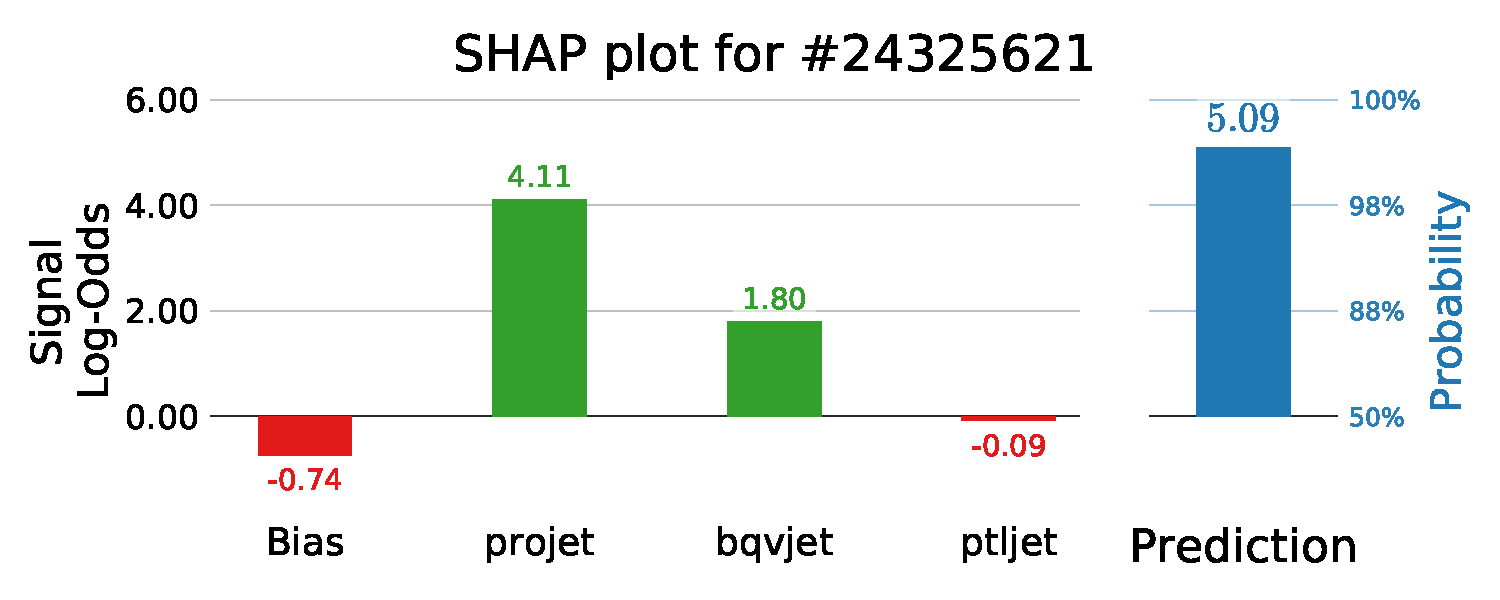
\includegraphics[width=0.95\textwidth, trim=0 0 0 40, clip]{figures/quarks/shap_values-down_sample=1.00-ML_vars=vertex-selection=b-ejet_min=4-n_iter_RS_lgb=99-n_iter_RS_xgb=9-cdot_cut=0.90-version=19-njet=3loc=24325621.pdf}
  \caption[SHAP 3-Jet Model Explanation for $b$\=/Like Jet]
          {Model explanation for the 3-jet $b$\=/tagging LGB model for a $b$\=/like jet. The first column is the bias which can be seen as the naive prediction baseline, the rest are the input variables. On the right hand side of the plot is the model prediction shown. The left part of the plot is shown in log-odds space, the right part in probability space. The \textcolor{red}{negative} log-odd values are shown in red, \textcolor{green}{positive} ones in green, and the \textcolor{blue}{prediction} value in blue. 
          } 
  \label{fig:q:shap_single_prediction_3j}
\end{figure}



\section[b-Tagging Efficiency]{$b$\=/Tagging Efficiency}
\label{sec:q:b_tagging_effiency}

Before any further analysis can be done, the efficiency of the $b$\=/tagging model has to be measured. The efficiency $\varepsilon$ is defined as the number of particles, events, jets, or any other countable measure, $N_\mathrm{sel}$, that are selected by the algorithm divided by the \emph{true} number, $N_\mathrm{truth}$:
\begin{equation}
  \varepsilon = \frac{N_\mathrm{sel}}{N_\mathrm{truth}}. 
\end{equation}
Of course, the truth is never known in Nature, however, it is for simulated MC events. The efficiency is used to estimate how many particles (e.g.) that were generated even though only a subset of the particles were detected. Imagine a hypothetical experiment where \num{21} particles were observed and the efficiency of the experiment was $\varepsilon=\SI{50}{\percent}$. This means that there were created $21 / \varepsilon = 42$ particles in the experiment, yet only \num{21} of them were observed.

For measuring the $b$\=/tagging efficiency we apply a Tag-Tag-Probe (TTP) method based on the $b$\=/tags. In 3-jet events two of the jets will serve as tags and the last one as probe. The tags are jets where, if they are known, the probe is also known (with high probability). One can then apply the cut to the probe and see if it would have passed the cut or not. This method provides a clean and unbiased sample (the probes) and since (with high probability) the truth of the probe jet is known, the efficiency can be measured in this way \autocite{atlascollaborationElectronEfficiencyMeasurements2017}. Since the TTP method does not depend on real truth, it can be used on both MC and Data.

To measure the $b$\=/tagging efficiency we use that the $Z$ decay has the form $Z \rightarrow q\bar{q}g$. Quantum field calculations based on the Standard Model predicts that the decay $Z \rightarrow ggg$ is extremely unlikely with a branching ratio of $\sim 10^{-6}$ \autocite{vanderbijBosonProductionDecay1989}. This decay was actually tested at LEP which did not find any $ggg$ events and concluded that the branching ratio was $< \SI{1.6}{\percent}$ with an upper limit at \SI{95}{\percent} confidence level \autocite{damUpperLimitBr1996}. This number is further reduced today to $<\SI{1.1}{\percent}$ \autocite{particledatagroupReviewParticlePhysics2018}. 

That the $Z$ decays to $q\bar{q}g$ means that if one of the jets get a high $b$\=/tag (and is thus likely to be a $b$\=/jet), and another one of the jets gets a low $b$\=/tag (and is thus likely to be a $g$\=/jet), then it is highly probable that the remaining jet is a $b$\=/jet. To formalize this, sort the jets after their $b$\=/tags values from high to low such that $\beta_{\mathrm{tag}_1} > \beta_{\mathrm{tag}_2} > \beta_{\mathrm{tag}_3}$ for the jets $\vec{J}=[J_1, J_2, J_3]$ where $J_i$ has $b$\=/tag $\beta_{\mathrm{tag}_i}$. We then define the two tags $T_b$ and $T_g$ as $\vec{J}=[T_b, P, T_g]$ where $P$ is the probe. If the two tags $T_b$ and $T_g$ passes the cuts $\beta_{b\dash\mathrm{cut}} < \beta_{\mathrm{tag}_1}$ and $\beta_{\mathrm{tag}_3} < \beta_{g\dash\mathrm{cut}}$, then the probe is selected $P=J_2$. If the probe is selected, then the last cut $\beta_{b\dash\mathrm{cut}} < \beta_{\mathrm{tag}_2}$ is the one that the efficiency is based on.

Based on Figure~\ref{fig:q:btag_histogram_4j} we define the threshold for the $b$\=/jet tag to be $\beta_{b\dash\mathrm{cut}}=0.9$ and for the $g$\=/jet to be $\beta_{g\dash\mathrm{cut}} = 0.4$. The $b$\=/signal region is thus $0.9 < \beta$ and the $g$\=/signal region $\beta < 0.4$ . With these cuts, the efficiency, denoted $\varepsilon_b^{b\dash\mathrm{sig}}$, of the $b$\=/jets being tagged as $b$\=/signal is computed. The TTP method is applied to both Data (Data TTP) and MC (MC TTP), along with a measurement of the efficiency when measured using MC truth (MC Truth) and a measurement based on the probes that were actual $b$\=/jets according to truth (MC Truth TTP)\sidenote{So the probes are selected by the TTP method, however, only true $b$-jet probes are kept.}. The efficiency is measured as a function of jet energy $E_\mathrm{jet}$ to gauge the energy dependence of the efficiency, i.e. computed in a bin-by-bin basis split according to the jet energy (of the probe). 

The efficiencies can be seen in Figure~\ref{fig:q:effiency_btag_bjet_bsig}. The efficiency $\varepsilon_b^{b\dash\mathrm{sig}}$ as a function of jet energy $E_\mathrm{jet}$ can be seen on the left $y$\=/axis, whereas the number of probes in each bin $N_\mathrm{truth}$ can be seen on the right $y$\=/axis. The efficiencies increase as a function of energy and reaches a plateau at $E_\mathrm{jet} \sim \SI{30}{\GeV}$: high-energy $b$\=/jets are easier to classify than low-energy ones. 
Even though the efficiencies of the MC TTP and Data TTP methods are lower than the MC Truth and MC Truth TTP, the important thing to notice is that they follow each other closely, an indicator of the trained $b$\=/tagging model working equally well on both MC and Data (as hoped).  

\begin{figure}[h!]
  \centerfloat
  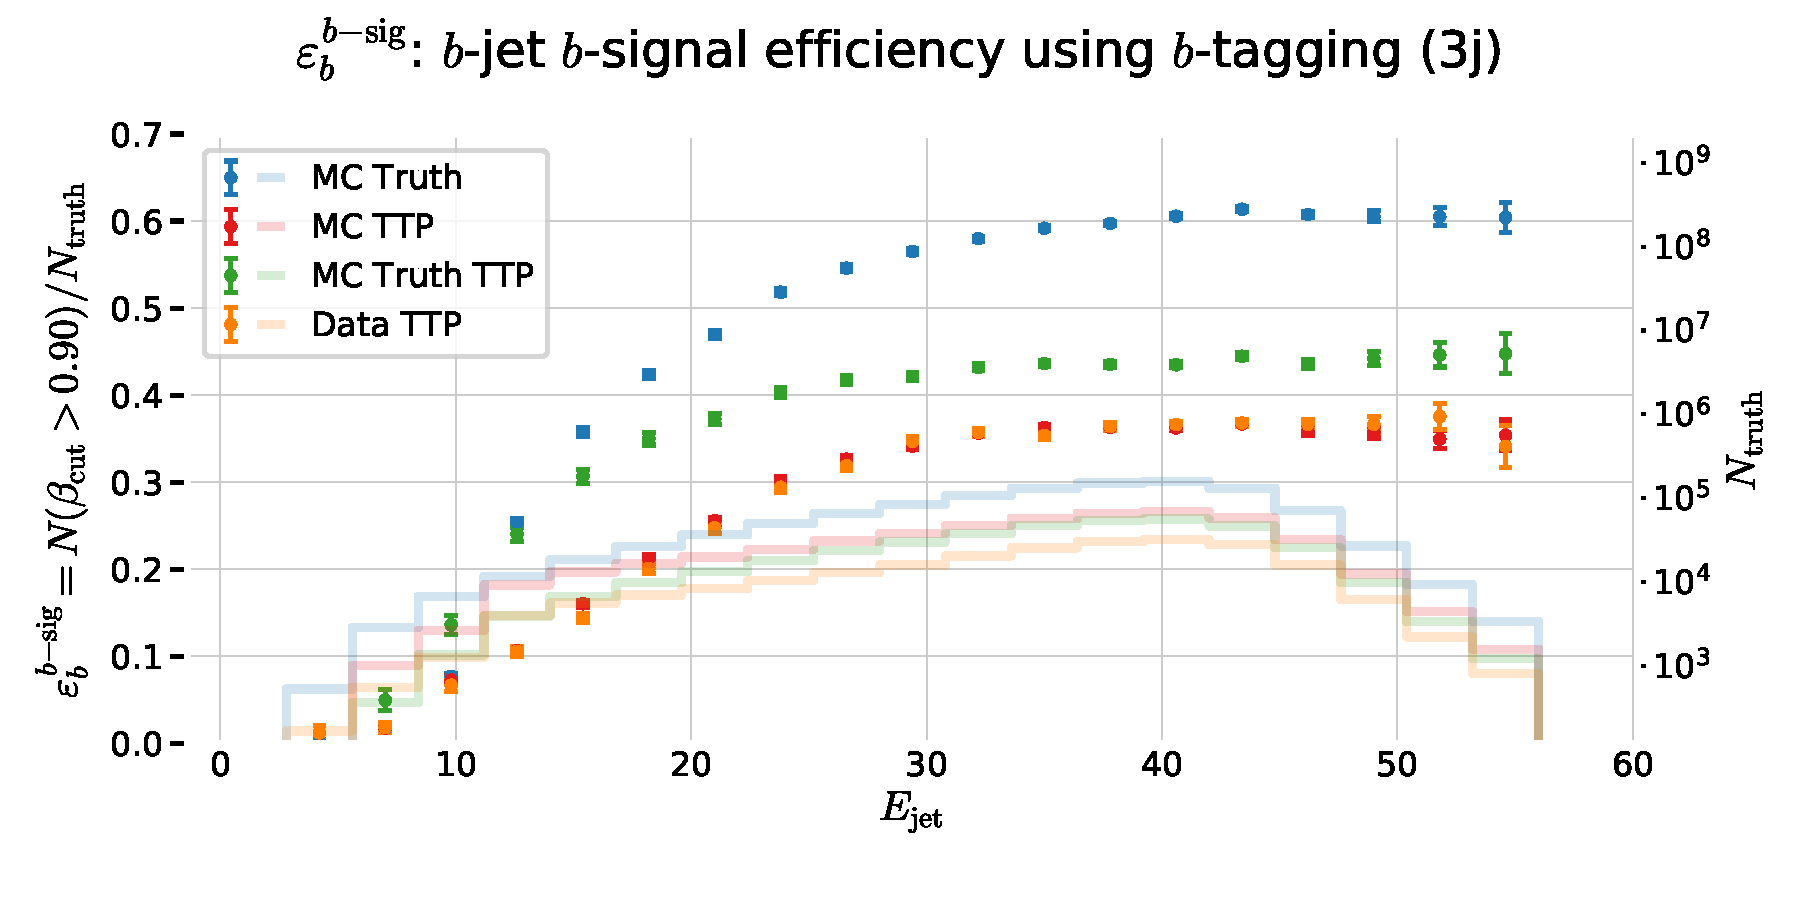
\includegraphics[width=1.1\textwidth, trim=20 30 0 40, clip]{figures/quarks/eff_b_bsig-down_sample=1.00-ML_vars=vertex-selection=b-ejet_min=4-n_iter_RS_lgb=99-n_iter_RS_xgb=9-cdot_cut=0.90-version=19.pdf}
  \caption[$b$\=/Tagging Efficiency $\varepsilon_b^{b\dash\mathrm{sig}}$ as a Function of Jet Energy]
          {$b$\=/tag efficiency for $b$\=/jets in the $b$\=/signal region for 3-jet events, $\varepsilon_b^{b\dash\mathrm{sig}}$, as a function of jet energy $E_\mathrm{jet}$. In the plot the efficiencies are shown for \textcolor{blue}{MC TTP} in blue, \textcolor{red}{Data TTP} in red, \textcolor{green}{MC Truth TTP} in green, and \textcolor{orange}{MC Truth TTP} in orange. The efficiencies (the errorbars) can be read off on the left $y$\=/axis and the counts (histograms) on the right $y$\=/axis. Notice how both MC TTP and Data TTP follow each other closely.} 
  \label{fig:q:effiency_btag_bjet_bsig}
\end{figure}

The efficiency of $g$\=/jets in the $g$\=/jet signal region $\varepsilon_g^{g\dash\mathrm{sig}}$ based on the $b$\=/tags can be measured in a similar manner. Again TTP method is used, however, now the two $b$\=/jets are the tags and the $g$\=/jet is the probe. The cuts are the same as before, however, now it is required that $0.9 < \beta_{\mathrm{tag}_1}$ and $0.9 < \beta_{\mathrm{tag}_2}$ before the probe is selected $P=J_3$. The efficiency is then based on $\beta_{\mathrm{tag}_3} < 0.4 = \beta_{g\dash\mathrm{cut}}$. The efficiency $\varepsilon_g^{g\dash\mathrm{sig}}$ is plotted in Figure~\ref{fig:q:effiency_btag_gjet_gsig}. Here the MC TTP and Data TTP also follow each other closely, this time to around $\sim \SI{25}{\GeV}$.

Both of the efficiencies so far, $\varepsilon_b^{b\dash\mathrm{sig}}$ and $\varepsilon_g^{g\dash\mathrm{sig}}$, can be seen as signal efficiencies. Likewise, there are two background efficiencies, one for $b$\=/jets in the $g$\=/signal region $\varepsilon_b^{g\dash\mathrm{sig}}$ seen in Figure~\ref{fig:q:effiency_btag_bjet_gsig} and one for $g$\=/jets in the $b$\=/signal region $\varepsilon_g^{b\dash\mathrm{sig}}$ seen in Figure~\ref{fig:q:effiency_btag_gjet_bsig}.

\begin{figure}
  \centerfloat
  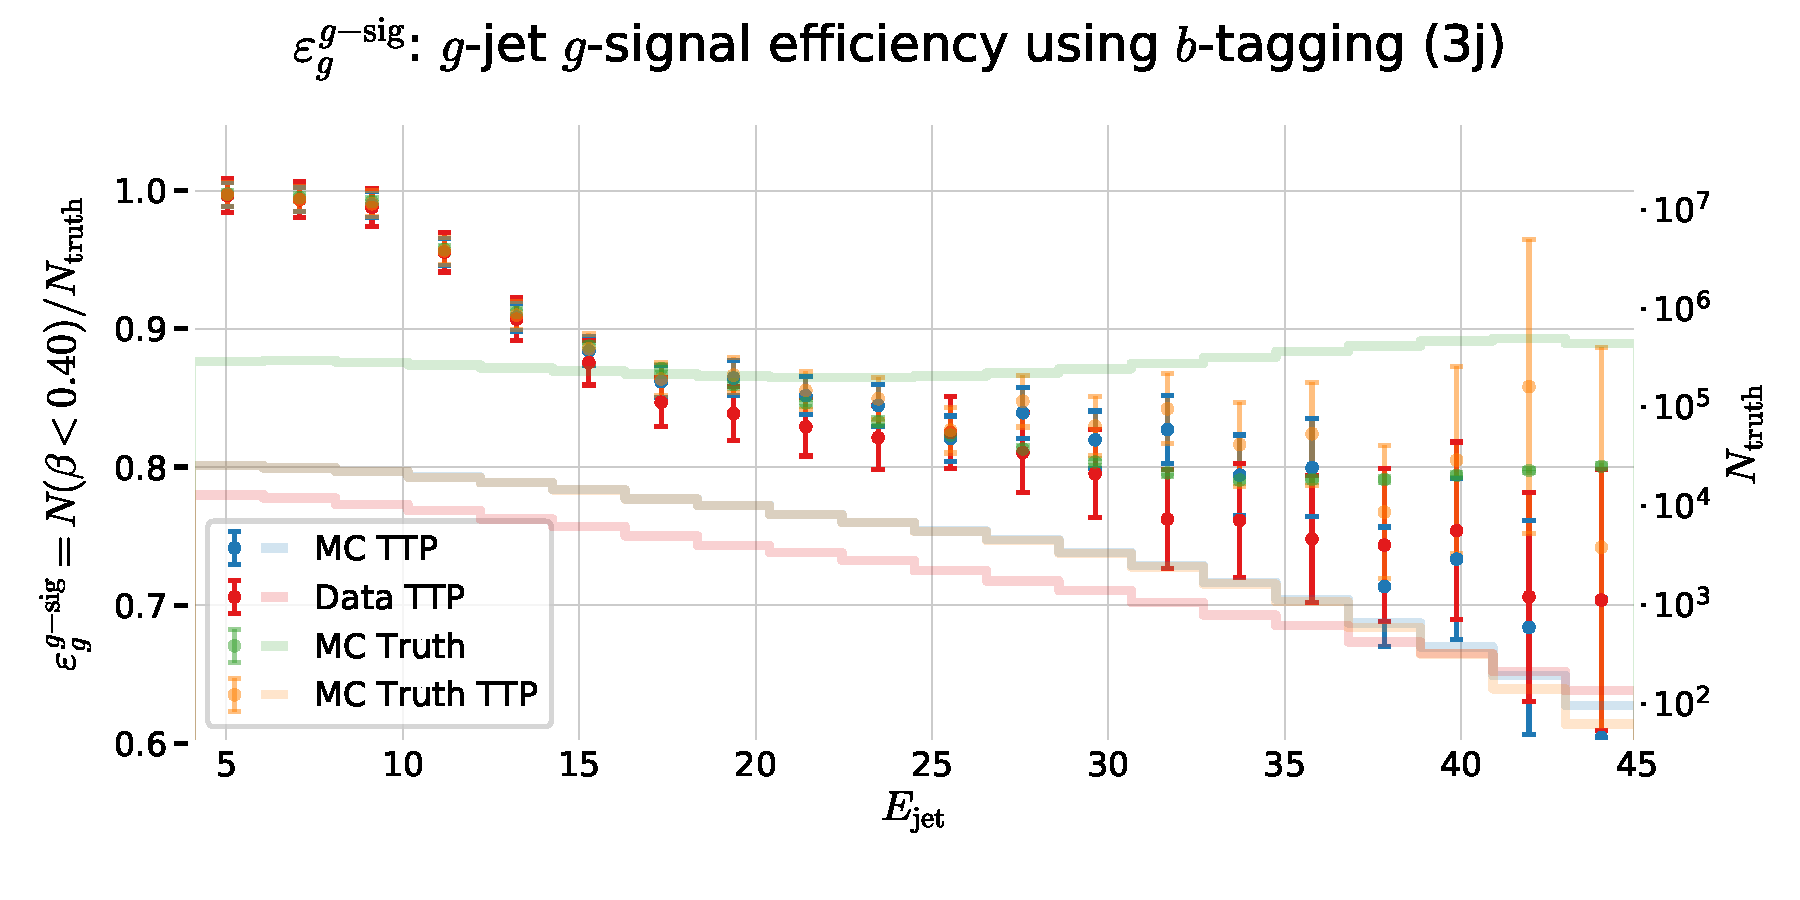
\includegraphics[width=1.1\textwidth, trim=20 30 0 40, clip]{figures/quarks/eff_g_gsig-down_sample=1.00-ML_vars=vertex-selection=b-ejet_min=4-n_iter_RS_lgb=99-n_iter_RS_xgb=9-cdot_cut=0.90-version=19.pdf}
  \caption[$b$\=/Tagging Efficiency $\varepsilon_g^{g\dash\mathrm{sig}}$ as a Function of Jet Energy]
          {$b$\=/tag efficiency for $g$\=/jets in the $g$\=/signal region for 3-jet events, $\varepsilon_g^{g\dash\mathrm{sig}}$, as a function of jet energy $E_\mathrm{jet}$. In the plot the efficiencies are shown for \textcolor{blue}{MC TTP} in blue, \textcolor{red}{Data TTP} in red, \textcolor{green}{MC Truth TTP} in green, and \textcolor{orange}{MC Truth TTP} in orange. The efficiencies (the errorbars) can be read off on the left $y$\=/axis and the counts (histograms) on the right $y$\=/axis. Notice how both MC TTP and Data TTP follow each other closely until $\sim \SI{25}{\GeV}$.} 
  \label{fig:q:effiency_btag_gjet_gsig}
\end{figure}

This section shows that the $b$\=/tagging efficiencies of the LGB $b$\=/tagging model shows comparable performance on both MC and Data which indicates that the model is un-biased (w.r.t. energy).

\FloatBarrier
\section[g-Tagging Analysis]{$g$\=/Tagging Analysis}
\label{sec:q:g_tagging_analysis}

The $b$\=/tagging model is a jet-based model which provides a $b$\=/tag score $\beta_\mathrm{tag}$ to a jet. This also means that each of the jets in e.g. a 4-jet event can get a $b$\=/tag: $\bm{\beta}_\mathrm{tag}=[\beta_{\mathrm{tag}_1}, \beta_{\mathrm{tag}_2}, \beta_{\mathrm{tag}_3}, \beta_{\mathrm{tag}_4}]$. Treating $\bm{\beta}_\mathrm{tag}$ as an individual observation, one can train a new model on the events based on the events compared to the individual jets. 
% This model will be called the $g$-tagging model. 
This event-based process will be called $g$\=/tagging and the trained model will return a $g$\=/tag score written as $\gamma_\mathrm{tag}$.

For this model, signal events are defined to be events which are $q$\=/matched\sidenote{Remember that $q$\=/matched events are events with one, and only one, jet that is $q$\=/matched to one of the quark-jets, and one, and only one of the jets is $q$\=/matched to the other quark-jet.} and where the two jets with the highest $b$-tags are matched to the two (final) quark jets. Another way to say this, is that the non\=/$q$\=/matched jets are assigned the $n-2$ lowest $b$\=/tag scores for $n$\=/jet events. An example of a signal event is $\bm{\beta}_\mathrm{tag}=[0.95, 0.89, 0.15, 0.07]$ for an event with the four jets $[b, \bar{b}, g, g]$. Compared to the $b$\=/tagging model, this model will allow one to extract entire events which contains a clear identification of gluons versus non-gluons.

\subsection{Permutation Invariance}
\label{subsec:q:permutation_invariance}

Since the $b$\=/tags are only based on the vertex variables, the goal of the $g$\=/tag is to also be constructed in an un-biased way with respect to the jet energy $E_\mathrm{jet}$. However, even though $\beta_\mathrm{tag}$ is independent of $E_\mathrm{jet}$ and $\gamma_\mathrm{tag}$ is a function of $\beta_\mathrm{tag}$, it turned out that $\gamma_\mathrm{tag}$ was not independent of $ E_\mathrm{jet}$. This was because the ordering of the jets within the event was energy-dependent: they are sorted according to their $E_\mathrm{jet}$. 

This meant that the different variables ($b$-tags) in $\bm{\beta}_\mathrm{tag}$ had different feature importances when tested, even though they should be equally important. Instead of defining $\bm{\beta}_\mathrm{tag}$ as a vector it should instead be seen as a set\sidenote{Since sets have no inherent order.} $\bm{\beta}_\mathrm{tag} \equiv \{\beta_{\mathrm{tag}_1}, \dots, \beta_{\mathrm{tag}_n}\}$. The $g$\=/tagging model trained on the events should thus be \emph{permutation invariant}\sidenote{$f(\vec{x}) = f(\tau(\vec{x}))$ for any permutation $\tau$ on an input vector $\vec{x}$.} with regards to the input variables. The category of permutation invariant (and equivariant\sidenote{$\tau(f(\vec{x})) = f(\tau(\vec{x}))$ for any permutation $\tau$ on an input vector $\vec{x}$.}) neural networks has seen an huge development within recent years in the deep learning community. The paper from \citet{zaheerDeepSets2017} in \num{2017} was highly influential, however also other examples exists \autocite{ravanbakhshDeepLearningSets2017, guttenbergPermutationequivariantNeuralNetworks2016}. Yet, the same development cannot be said to have happened within the more classic machine learning field.

Although not being a novel software-technical solution, I circumvent the problem with two simple different approaches: 1) by simply shuffling the inputs variables independently for each observation (row) in the dataset, and 2) training on all possible permutations of the variables in the dataset. The second approach can be seen as a feature augmentation technique where the data is artificially increased with factor of $n$ factorial: $N \rightarrow n!\cdot N$ where $N$ is the number of events and $n\in \{3, 4\}$ is the number of jets. These two methods were tested along with keeping the original order of the dataset. 

% \vspace{-2cm} 

\subsection{Truncated Uniform PDF}
\label{subsec:q:trunc_uniform}

Initially when plotting the HPO performance as a function of iteration, it was seen how there were some very clear plateaus, where the highest plateau (i.e. the highest AUC value and thus the best score) was only seen in the very first iteration. It was quickly realized that this was due to the very first iteration was being run with the default values of the LGB in my HPO setup. However, what was not understood was why this value was performing so much better than the different sets of hyperparameters in the random search. Of course LightGBM have chosen their default parameters wisely, however, one would not expect them to outperform other sets of hyperparameters that clearly. During the debugging process, the column downsampling \code{colsample_bytree} was diagnosed to be the culprit. 

The default value is \code{colsample_bytree}$=1$, however, the probability density function (PDF) used in random search for this parameter was $\mathcal{U}(0.4, 1)$ which was expected to give the same performance as the default value, at least for values of \code{colsample_bytree} close to \num{1}. By inspecting the source code of LightGBM, I realized that if the column downsampling is less than \num{1} the model takes the integer of the column downsampling multiplied with the total number of columns (variables/features) \autocite{MicrosoftLightGBM}. This means that no matter how close to \num{1} the column downsampling get, the integer value of the total number of columns get floored to {maximally} \num{2} in 3-jet events, compared to when the column downsampling is exactly \num{1} (which it only is for the default values).

To deal with this problem I developed a new PDF\sidenote{Not strictly a PDF since it is not normalized, but otherwise behaves as one.} on top of the existing ones in Scipy: the truncated uniform PDF $\mathcal{U}_\mathrm{trunc}(a, b, c)$. This PDF first generates a random number $x$ from a uniform distribution between $a$ and $c$. Then, if $x$ is larger than $b$ it is floored to $b$. In this way, it is possible to both get values of $x$ in the interval $[a, b]$ but also values exactly equal to $b$. The value of $c$ controls how often these \q{overflow} values of $x$ are generated.

\subsection{$g$\=/Tagging Hyperparameter Optimization}

Four LightGBM models, two for 3-jet events and two for 4-jet events, were trained and hyperparameter optimized for both the the energy ordered and shuffled data sets with \num{100} iterations of random search. The method with all permutations was trained using the same hyperparameters as the best ones founds in the HPO for the shuffled model to reduce time\sidenote{The time performance is extra important for the method with all permutations as the dataset is \num{24} times larger the method with the shuffling for 4-jet events.} spent on HPO. The same PDFs as for the $b$\=/tagging were used, see Table~\ref{tab:q:hpo_ranges_lgb}, and $5$\=/fold cross validation and early stopping was applied with a patience of \num{100}. 

\begin{figure*}[h!]%
  \centerfloat
  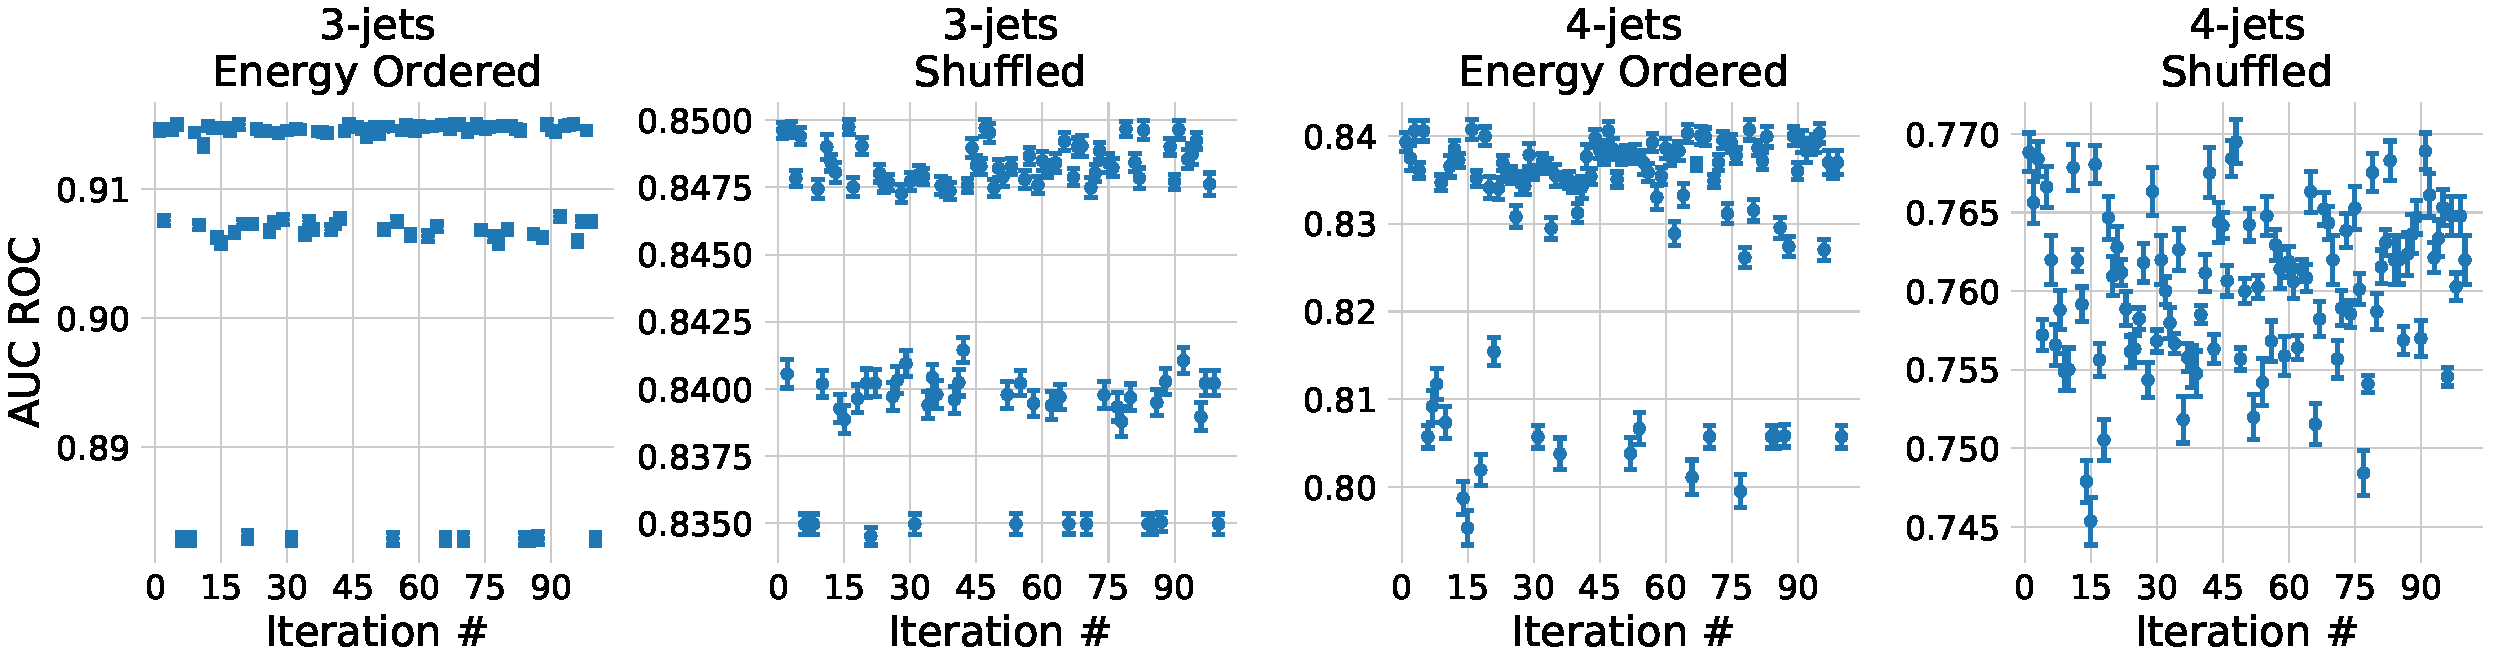
\includegraphics[width=1\textwidth, trim=0 0 0 0, clip]{figures/quarks/cv_res_lgb-gtag-down_sample=1.00-ML_vars=vertex-selection=b-ejet_min=4-n_iter_RS_lgb=99-n_iter_RS_xgb=9-cdot_cut=0.90-version=19.pdf}
  \vspace{3mm}
  \caption[Hyperparameter Optimization of $g$\=/Tagging]{
    Hyperparameter Optimization results of $g$\=/tagging with \num{100} iterations of random search with LGB. From left to right, we have A) 3-jet events energy-ordered (no permutations), B) 3-jet events row-shuffled, C) 4-jet events energy-ordered, D) 4-jet events row-shuffled. Notice the different ranges on the y-axes.}
  \label{fig:q:CV_res_iterations_g_tagging}%
\end{figure*}
\vspace{-3mm}

The results of the HPO can be seen in Figure~\ref{fig:q:CV_res_iterations_g_tagging}. Here the two 3-jets models are seen in the two plots to the left, and the two 4-jets to the right. The very left plot shows the performance as a function of iteration number for the 3-jet energy-ordered method (no permutation or shuffling). This was where the issues mentioned in \autoref{subsec:q:trunc_uniform} were first discovered. There are three very noticeable plateaus in this plot which corresponds to running column subsampling with zero, one, or two variables dropped. The three plateaus are also seen in the 3-jet events that were shuffled, however, with more variation in each plateau (along with a drop in performance). For the 4-jet events the plateaus are not as apparent but it can still be seen how some of the iteration show a significantly lower score than others. The parallel coordinate plots for the four plots can be seen in Figure~\ref{fig:q:CV_res_parallel_coords_g_tag_3j_energy_ordered}--\ref{fig:q:CV_res_parallel_coords_g_tag_4j_shuffled}.

The global SHAP feature importances $\phi^\mathrm{tot}_{\beta_\mathrm{i}}$ are computed for each one of the three methods, energy-ordered, shuffled, or with all permutations, to verify their permutation invariance properties. The results are seen in Table~\ref{table:q:shap_g_taggging_global_4j} for 4-jet events and in Table~\ref{table:q:shap_g_taggging_global_3j} for 3-jet events. 

\begin{table}[h!]
  \centerfloat
  \begin{tabular}{@{}rccc@{}}
  ${\beta_\mathrm{tag}}_i$  & Energy Ordered & Shuffled & All Permutations \\ \midrule
  $i=1$ & $ 0.986 \pm 0.008 $  &  $ 0.474 \pm 0.005 $  &  $ 0.465 \pm 0.005 $  \\
  $i=2$ & $ 0.609 \pm 0.006 $  &  $ 0.467 \pm 0.005 $  &  $ 0.464 \pm 0.005 $  \\
  $i=3$ & $ 0.424 \pm 0.004 $  &  $ 0.461 \pm 0.005 $  &  $ 0.452 \pm 0.005 $  \\
  $i=4$ & $ 0.244 \pm 0.002 $  &  $ 0.481 \pm 0.005 $  &  $ 0.466 \pm 0.005 $  \\ 
  \end{tabular}
  \caption[Global SHAP Feature Importances for the $g$\=/Tagging Models in 4-Jet Events]{Global SHAP feature importances $\phi^\mathrm{tot}_{\beta_\mathrm{i}}$ for the three $g$\=/tagging models in 4-jet events. Each $\phi^\mathrm{tot}_{\beta_\mathrm{i}}$ is shown for the three methods in the columns and the four $b$\=/tags as variables in the rows.}
  \label{table:q:shap_g_taggging_global_4j}
\end{table}
\vspace{2mm}

Here it can be seen that the model trained on the energy ordered data learned to attribute the highest weight to the first $b$\=/tag, second highest weight to the second $b$\=/tag, and so on. In contrary, the weights are uniformly distributed between the different $b$\=/tags in both the shuffled and all-permuted datasets (within a few sigma). The same overall pattern is seen for the 3-jet events. Based on the tables, it can be seen that both the shuffling method and all-permuting method are methods for training ML models with permutation invariant properties due to their approximately equal attribution of weight to the different variables ($b$-tags). 



\subsection{PermNet}
\label{subsec:q:permnet}

In addition to the LGB models, a permutation invariant neural network called PermNet based on the Deep Sets paper \autocite{zaheerDeepSets2017} implemented in Tensorflow \citep{tensorflow2015-whitepaper} by \citet{fayeFrederikFayeDeepcalo} was also tested. \citet{zaheerDeepSets2017} showed that $f(X)$ is permutation invariant if and only if it can be decomposed in the following way:
\begin{equation}
  \label{eq:q:deep_sets}
  f(X)=\rho\left(\sum_{x\in X} \phi(x) \right).
\end{equation}
for suitable transformations $\rho$ and $\phi$ which the neural network learns. This is possible since neural networks are universal function approximators \autocite{hornikApproximationCapabilitiesMultilayer1991}. The PermNet was trained using three layers\sidenote{Where the two hidden layers have \num{128} and \num{64} neurons in each.} with leaky ReLU \autocite{Maas2013RectifierNI} as the activation function and ADAM \autocite{kingmaAdamMethodStochastic2014} as the optimizer optimizing the log-loss. The network was trained with early stopping with a patience of \num{50} epochs and a batch size of \num{128}. A visual overview of the PermNet architecture can be seen in Figure~\ref{fig:q:permnet_architecture}. It took around \num{6} hours to fit the 3-jet events and \num{4.5} hours for the 4-jets (due to fewer events) for each of the models.

\subsection{1D Comparison of LGB and PermNet}
\label{subsec:q:lgb_permnet_comparison}

I made a small study to better understand the LGB and (especially) the PermNet models. This comparison was constructed by summing the $b$\=/tag scores in the $n$\=/jet event together $\sum_i^n \beta_{\mathrm{tag}_i}$. The $\beta_{\mathrm{tag}_i}$ are summed together since this turns the problem into a \num{1}D problem that is easy to visualize, the sum of numbers is a permutation invariant function. The sum also corresponds to the simplest functions of $\rho$ and $\phi$ in equation \eqref{eq:q:deep_sets}: the identity function. Both 1D models are fit to the training events. After the fits, a linear scan from $\sum_i^n \beta_{\mathrm{tag}_i}=0.4$ to $3.1$ is made to see how the predicted $g$\=/tags distribute. This is shown in Figure~\ref{fig:q:1d_sum_models_signal_fraction_4j} for 4-jet events. Here the value of $\gamma_\mathrm{tag}$ is shown for the two models together with the fraction of signal to background in each bin. If the $g$\=/tag score should resemble a true probability it would be expected to follow the signal ratio, e.g. a model should predict $\gamma_\mathrm{tag}=0.9$ if there is \SI{90}{\percent} signal in that bin. In the figure it is seen how the PermNet does a great job at fitting the signal fraction and the LGB model also does a decent job. Remember that none of these models were shown the signal fraction explicitly, only the $b$\=/tag sum and a truth label. The distribution of signal and background\sidenote{Which the signal fraction is based on.} together with the distribution of cuts made by the LGB model can be seen in Figure~\ref{fig:q:1d_sum_model_cuts_4j}. The similar plots for 3-jet events are plotted in Figure~\ref{fig:q:1d_sum_models_signal_fraction_3j} and \ref{fig:q:1d_sum_model_cuts_3j}.

\begin{figure}
  \centerfloat
  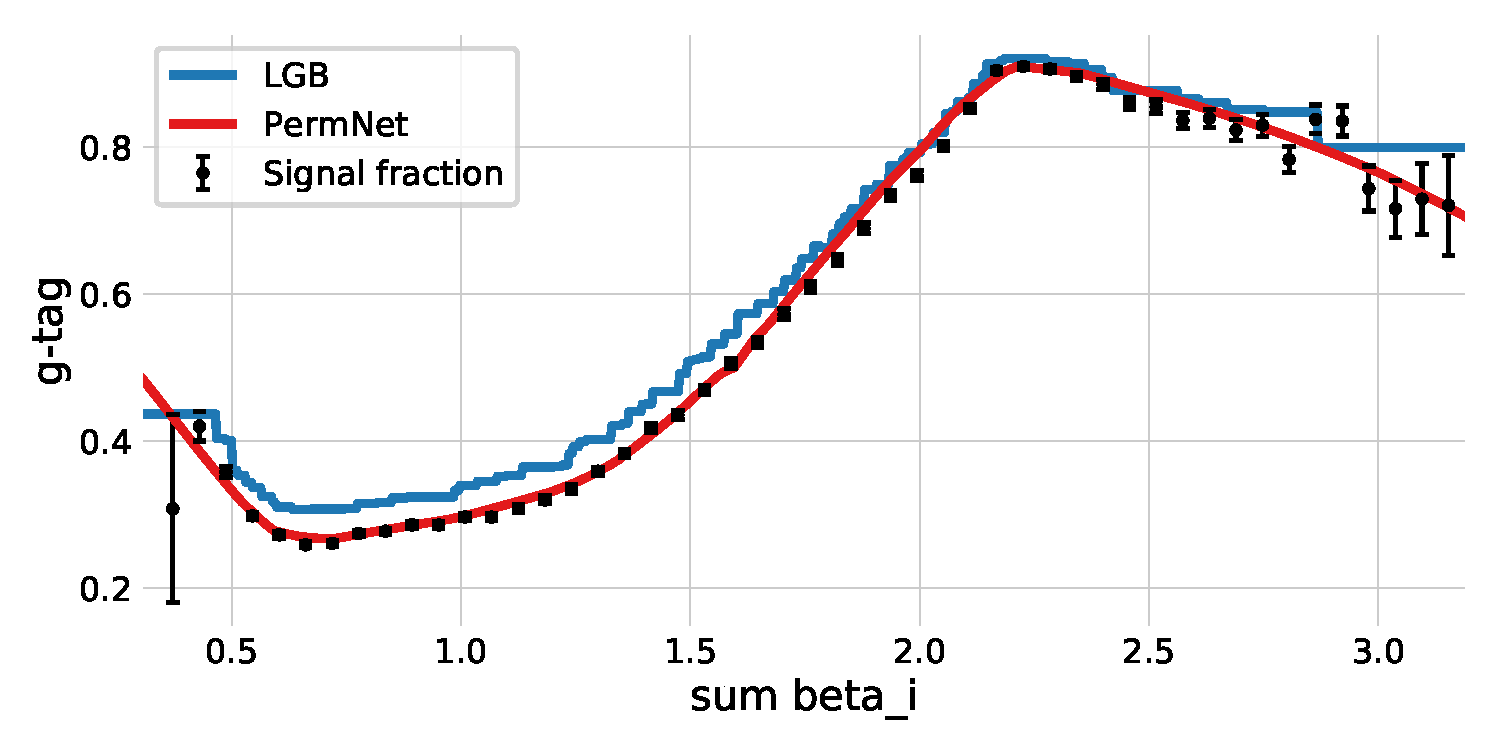
\includegraphics[width=0.95\textwidth, trim=10 10 10 20, clip]{figures/quarks/gtag_sum_models_njet=4-down_sample=1.00-ML_vars=vertex-selection=b-ejet_min=4-n_iter_RS_lgb=99-n_iter_RS_xgb=9-cdot_cut=0.90-version=19.pdf}
  \caption[1D Sum Models Predictions and Signal Fraction for 4-jets events]
          {Plot of the (1D) $g$\=/tag scores for 4-jet events as a function of $\sum \beta_i$ for the \textcolor{blue}{LGB} model in blue and the \textcolor{red}{PermNet} model in red. The signal fraction (based on the signal and background histograms in \figref{fig:q:1d_sum_model_cuts_4j}) is plotted as black error bars where the size of the error bars is based on the propagated uncertainties of the signal and background histogram assuming Poissonian statistics. } 
  \label{fig:q:1d_sum_models_signal_fraction_4j}
\end{figure}

It can be concluded, at least in 1D, that both LGB and PermNet are able to capture the inherent structure in the 1D

% data. First of all it is seen that the two 1D models follow each other relatively close and only predicts $\gamma_\mathrm{tag}$s in a quite limited range. The three other PermNet curves follow each other in such an extent that it is almost difficult to separated them, which is also expected since they should not be able to distinguish between the energy ordered and the shuffled events. The LGB models for the shuffled and all-permuted events 

\subsection{$g$\=/Tagging Results}

The distribution of $g$\=/tag scores in 4-jet (training) events the can be seen in Figure~\ref{fig:q:gtag_scores_4j} for the eight combinations of the two models (LGB and PermNet) and the four data sorting methods (energy ordered, (row) shuffled, all permutations, and the 1D sum.). At first the increased number of events (a factor of \num{24} for 4-jet events) with the all-permutation scheme is seen separating the two light green curves from the rest. The energy ordered LGB model is the combination which utilizes most of the $\gamma_\mathrm{tag}$\=/range, while the two 1D sum models have the most limited range, indicating that the models are more uncertain about their predictions. The energy ordered and shuffled PermNet models can more or less only be distinguished because the latter is plotted with dashed lines. This makes sense, since they are also expected to make the same predictions were they really permutation invariant\sidenote[][-0.7cm]{It is only because of the stochasticity in the optimization process of the two networks that they did not converge to exactly the same predictions.}. When plotted with normalized counts it is seen how the shuffled and all-permuted LGB models also follow each other very closely, which can still be partly seen in this plot by comparing the two distributions. The distribution of $g$\=/tags in 3-jet training events can be seen in Figure~\ref{fig:q:gtag_scores_3j}. 

\begin{figure}[ht]
  \centerfloat
  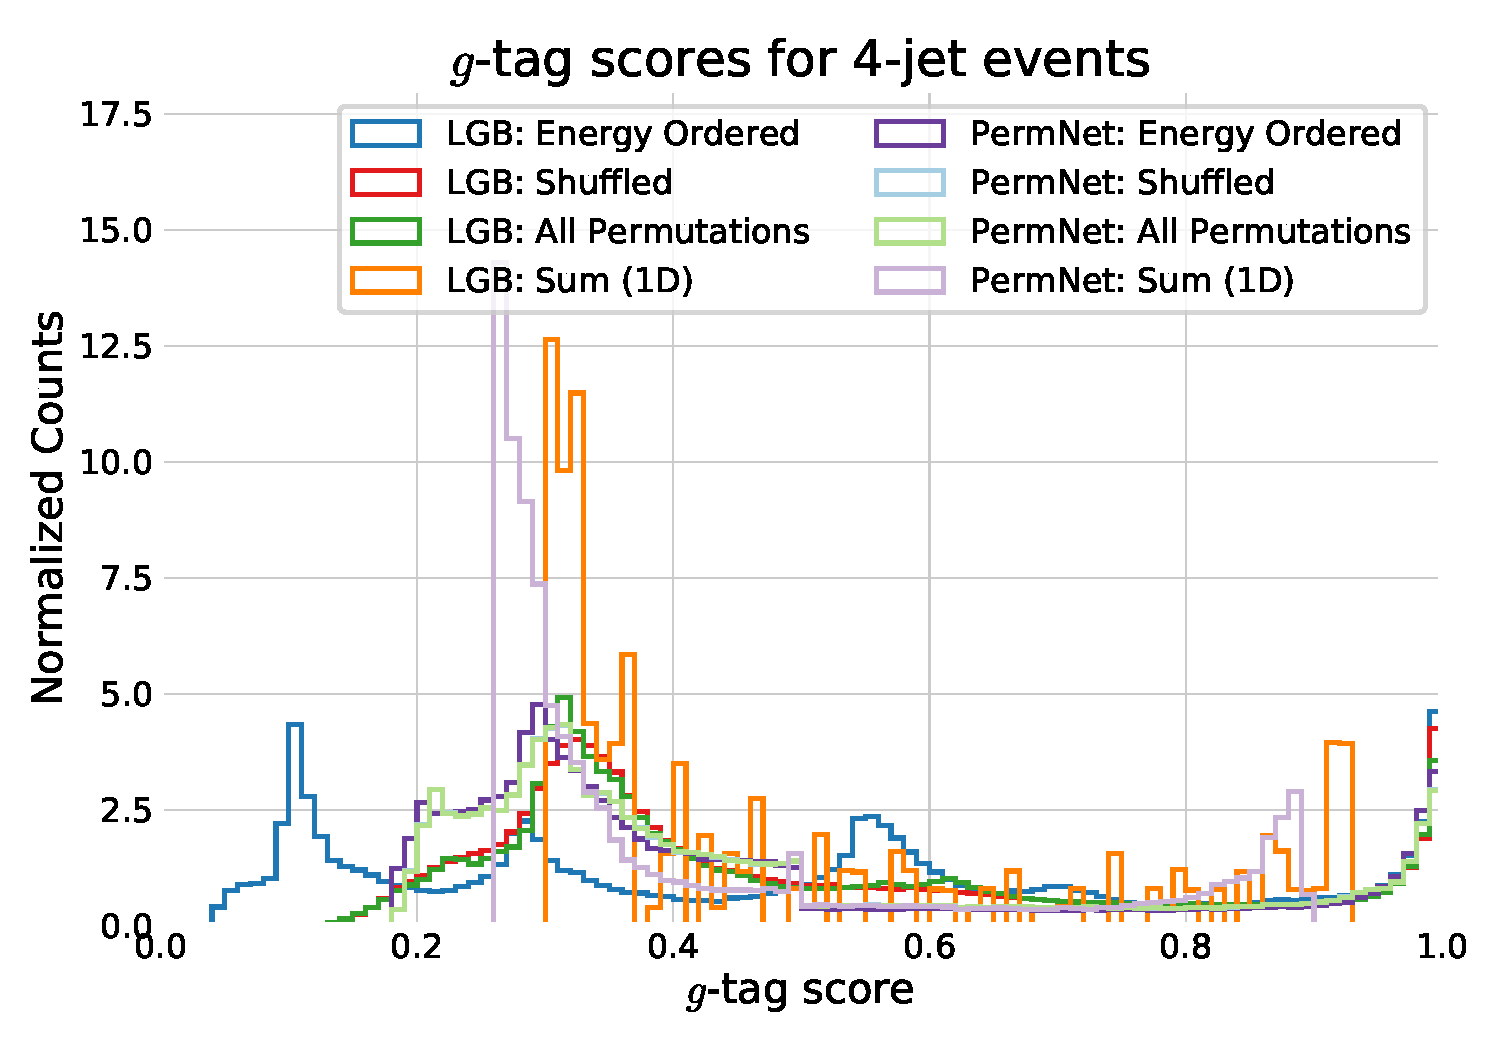
\includegraphics[width=0.95\textwidth, trim=10 10 10 45, clip]{figures/quarks/gtag_y_pred_4_jet_hist-down_sample=1.00-ML_vars=vertex-selection=b-ejet_min=4-n_iter_RS_lgb=99-n_iter_RS_xgb=9-cdot_cut=0.90-version=19.pdf}
  \caption[$g$\=/Tag Scores in 4-Jet Events]
          {Distribution of $g$\=/tag scores in 4-jet events shown with a logarithmic $y$\=/scale for LGB: Energy Ordered in blue, LGB: Shuffled in red, LGB: All Permutations in green, LGB: Sum 1D in orange, PermNet: Energy Ordered in purple, PermNet: Shuffled in light-blue, PermNet: All Permutations in light-green, PermNet: Sum 1D in light-purple.  Here LGB and PermNet are the two different type of models and \q{Energy Ordered}, \q{Shuffled}, \q{All Permutations}, and \q{Sum 1D} are the different methods used for making the input data permutation invariant (except energy ordered).}   
  \label{fig:q:gtag_scores_4j}
\end{figure}
% {Distribution of $g$\=/tag scores in 4-jet events shown with a logarithmic $y$\=/scale for \textcolor{blue}{LGB: Energy Ordered} in blue, \textcolor{red}{LGB: Shuffled} in red, \textcolor{green}{LGB: All Permutations} in green, \textcolor{orange}{LGB: Sum 1D} in orange, \textcolor{purple}{PermNet: Energy Ordered} in purple, \textcolor{light-blue}{PermNet: Shuffled} in light-blue, \textcolor{light-green}{PermNet: All Permutations} in light-green, \textcolor{light-purple}{PermNet: Sum 1D} in light-purple.  Here LGB and PermNet are the two different type of models and \q{Energy Ordered}, \q{Shuffled}, \q{All Permutations}, and \q{Sum 1D} are the different methods used for making the input data permutation invariant (except energy ordered).}   
\vspace{-3mm}

The ROC curve in Figure~\ref{fig:q:roc_gtag_4j_non_appendix} shows the performance of the different models on 4-jet events with the AUC shown in the legend. First of all it is easy to see that the energy ordered LGB model is significantly higher-performing than the rest of the models, however, this model is also energy-biased (not permutation invariant in the $b$\=/tags) and is only included to see how large a performance drop the permutation invariance criterion causes. The worst performing models are the two 1D sum models since they only have a single dimension to learn from, compared to the four dimensions that the other models have. Overall it can be seen that the rest of the models are performing almost identically, with the LGB model trained on all permutations to be the highest-performing of them all by a small margin. 
For 3-jet events a similar picture is seen, see Figure~\ref{fig:q:roc_gtag_3j}, however, here the LGB model trained on the shuffled events performs the best, yet this performance improvement is so small compared to the all-permutations LGB model that it is expected to be due to statistical fluctuations and not a real performance difference. 

\begin{figure}[h!]
  \centerfloat
  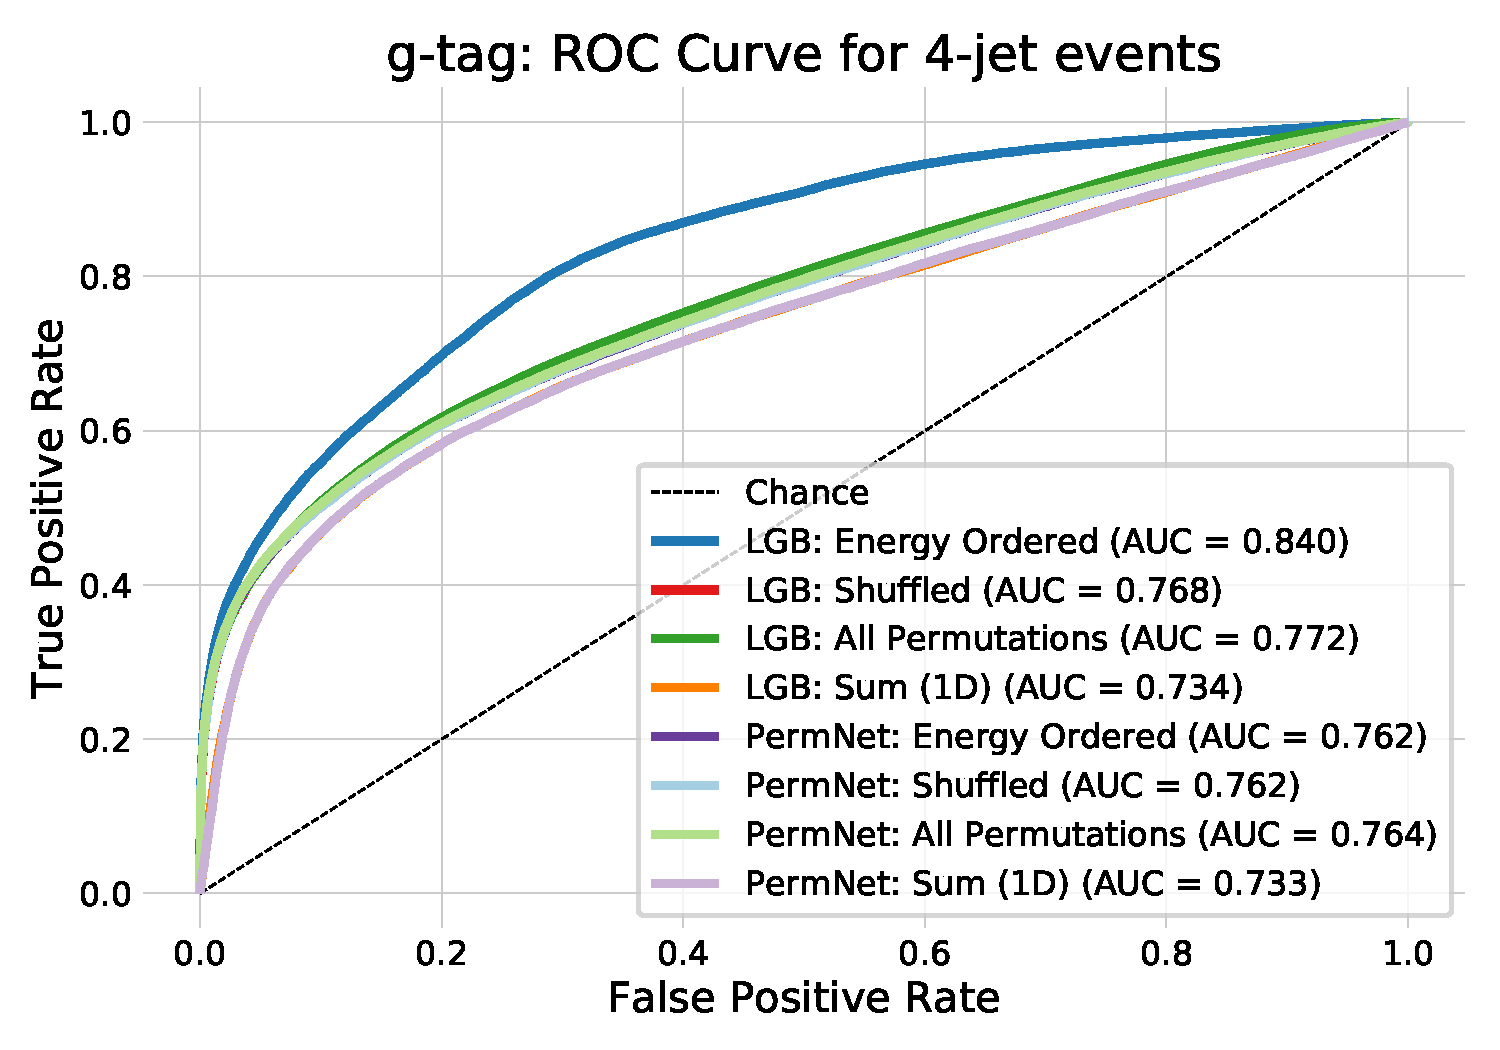
\includegraphics[width=0.95\textwidth, trim=10 10 10 40, clip]{figures/quarks/gtag_ROC_4_jet-down_sample=1.00-ML_vars=vertex-selection=b-ejet_min=4-n_iter_RS_lgb=99-n_iter_RS_xgb=9-cdot_cut=0.90-version=19.pdf}
  \caption[ROC Curve for $g$\=/Tag in 4-Jet Events]
          {\label{fig:q:roc_gtag_4j_non_appendix}ROC curve of the eight $g$\=/tag models in 4-jet events. First one in dashed black is the ROC curve that you get by random chance. The colors are the same as in 
          Figure \ref{fig:q:gtag_scores_4j} 
          and in the legend also the Area Under the ROC curve (AUC) is shown.} 
\end{figure}

Based on the AUC scores seen in the ROC curves in Figure~\ref{fig:q:roc_gtag_4j_non_appendix} and \ref{fig:q:roc_gtag_3j}, the LGB-model trained on all permutations will be the $g$\=/tagging model choice. To see how this model's predictions of the $g$-tags distribute for signal and background events, see Figure~\ref{fig:q:gtag_scores_4j_sig_bkg}. Here the distribution of $\gamma_\mathrm{tag}$ is shown for 4-jet signal events and background events. Remember that in $g$\=/tagging, the signal events are defined as events where the two jets with the highest $b$\=/tags are also the two $q$\=/matched jets (and the entire event is $q$\=/matched). In the figure it can be seen that at high values of $\gamma_\mathrm{tag}$ primarily $b\bar{b}gg$ events (signal $b$) are tagged where the jets are sorted according to their $b$\=/tags. Next after signal $b$ events is $c\bar{c}gg$ (signal $c$) and $bg\bar{b}g$\=/events\sidenote{Or any other permutation of $b$, $\bar{b}$, $g$, $g$ which is not $b\bar{b}gg$.} (background $b$). At low values of $\gamma_\mathrm{tag}$ light quarks ($uds$) dominate. 

\begin{figure}[h!]
  \centerfloat
  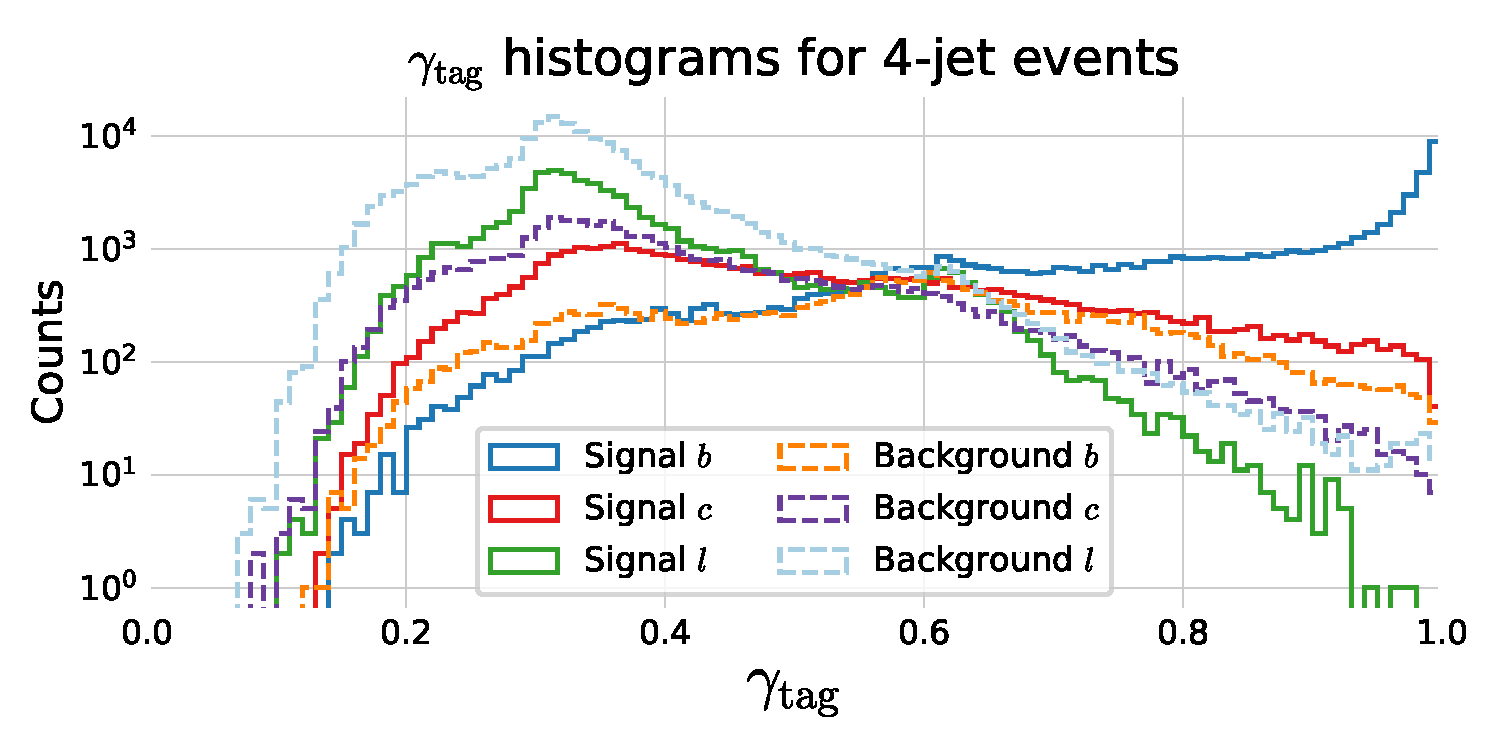
\includegraphics[width=0.9\textwidth, trim=10 10 10 45, clip]{figures/quarks/gtag-histogram-sigbkg-down_sample=1.00-ML_vars=vertex-selection=b-ejet_min=4-n_iter_RS_lgb=99-n_iter_RS_xgb=9-cdot_cut=0.90-version=19-njet=4.pdf}
  \caption[Distribution of $g$\=/Tag Scores in 4-Jet Events for Signal and Background]
          {Histogram of $g$\=/tag scores from the LGB-model in 4-jet events for \textcolor{blue}{$b$ signal} in blue, \textcolor{red}{$c$ signal} in red, \textcolor{green}{$l$ ($uds$) signal} in green, \textcolor{orange}{$b$ background} in orange, \textcolor{purple}{$c$ background} in purple, \textcolor{light-blue}{$l$ ($uds$) background} in light-blue.} 
  \label{fig:q:gtag_scores_4j_sig_bkg}
\end{figure}
\vspace{-3mm}

The similar plot for 3-jet events is seen in Figure~\ref{fig:q:gtag_scores_3j_sig_bkg}. This plot has some surprising bumps for mainly $l$\=/quark events. When comparing $l$\=/quark events in the high\=/$\gamma_\mathrm{tag}$ bump with the ones getting a low $\gamma_\mathrm{tag}$\=/value, see Figure~\ref{fig:q:gtag_scores_3j_l_quarks}, one can see that $l$\=/quark events with high $\gamma_\mathrm{tag}$ has only two jets with high $b$\=/tags, compared to low\=/$\gamma_\mathrm{tag}$ $l$\=/quark events which more often has three jets with high $b$\=/tags. 

\begin{figure}[h!]
  \centerfloat
  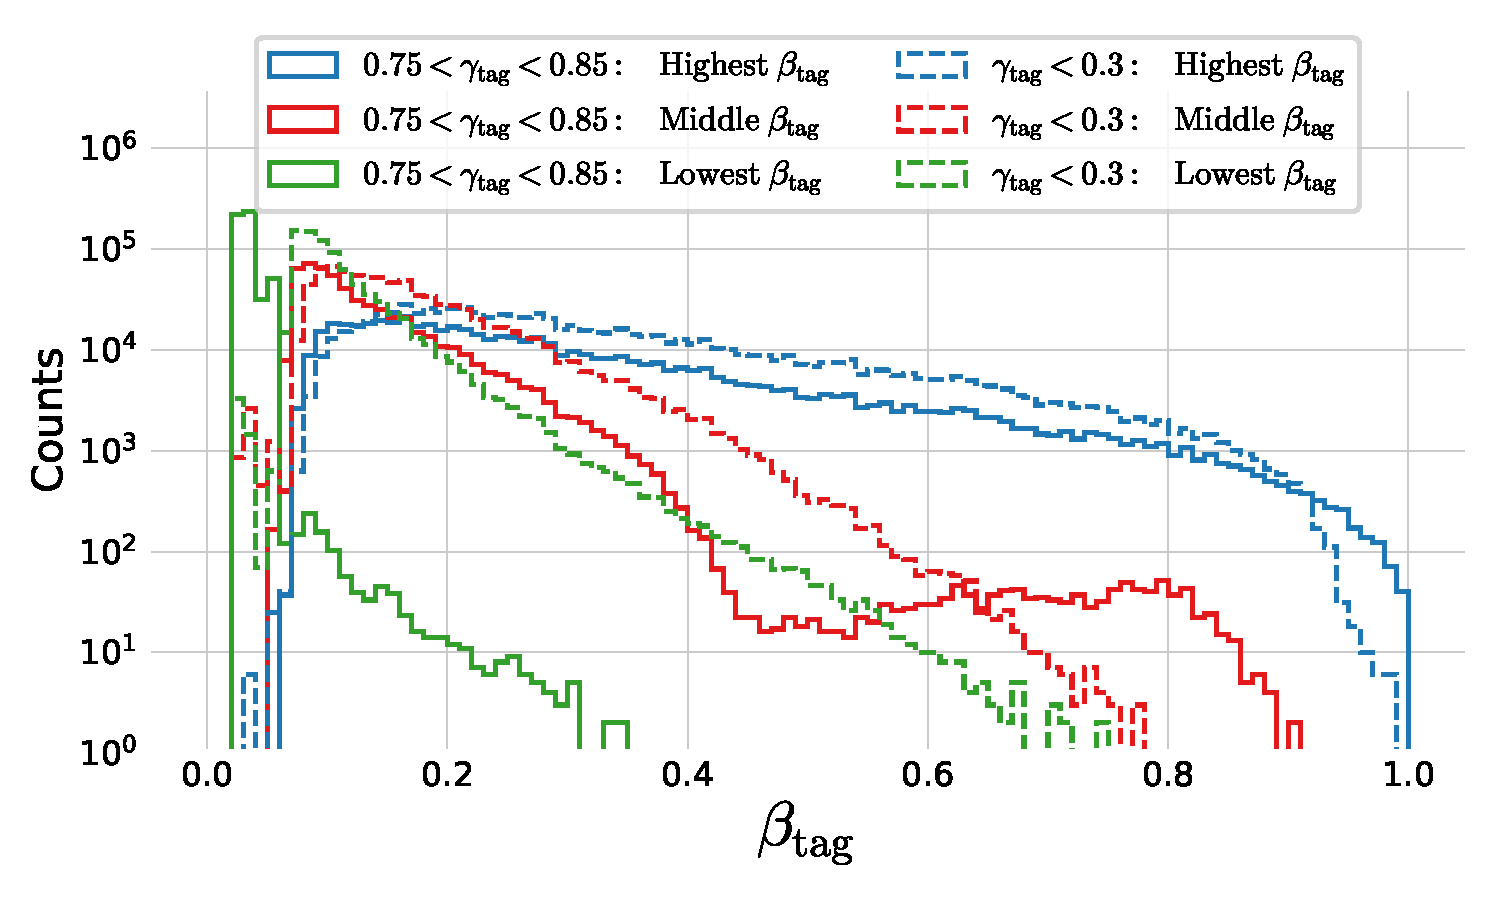
\includegraphics[width=0.95\textwidth, trim=10 10 10 10, clip]{figures/quarks/leptons_high_g_tag_3j_0.75_gtag_0.85-down_sample=1.00-ML_vars=vertex-selection=b-ejet_min=4-n_iter_RS_lgb=99-n_iter_RS_xgb=9-cdot_cut=0.90-version=19.pdf}
  \caption[Distribution of $b$\=/Tag Scores in 3-Jet $l$\=/Quark Events for Low and High $g$\=/Tag Values]
          {Distribution of $b$\=/Tag Scores in 3-Jet $l$\=/Quark Events for low and high $g$\=/tags values. Here $l$\=/quark events with $0.75 < \gamma_\mathrm{tag} <  0.85$, so the high peak in Figure~\ref{fig:q:gtag_scores_3j_sig_bkg}, are plotted in fully connected lines, and events with $\gamma_\mathrm{tag} <  0.3$ are plotted in dashed lines. For each of these two selection of events the value of the jet with the \textcolor{blue}{highest $\beta_\mathrm{tag}$} is shown in blue, the jet with the \textcolor{red}{middle $\beta_\mathrm{tag}$} in red, and the jet with the \textcolor{green}{lowest $\beta_\mathrm{tag}$} in green.} 
  \label{fig:q:gtag_scores_3j_l_quarks}
\end{figure}

This is even more visible once seen in a 3D scatter plot with the lowest $\beta_\mathrm{tag}$ on the $x$\=/axis, the middle on the $y$\=/axis, and highest on the $z$\=/axis. Three small views from the 3D visualization can be seen in Figure~\ref{fig:q:gtag_scores_3j_l_quarks_3d}. Here it is easily seen how the separating variable is the lowest $b$\=/tag: if an event where all three jets have high $b$\=/tags are used as input to the $g$\=/tagging model it gives it a low $g$\=/tag compared to if only two of the three jets have high $b$\=/tags.

\begin{figure*}[h!]
  \centering
  \subfloat{{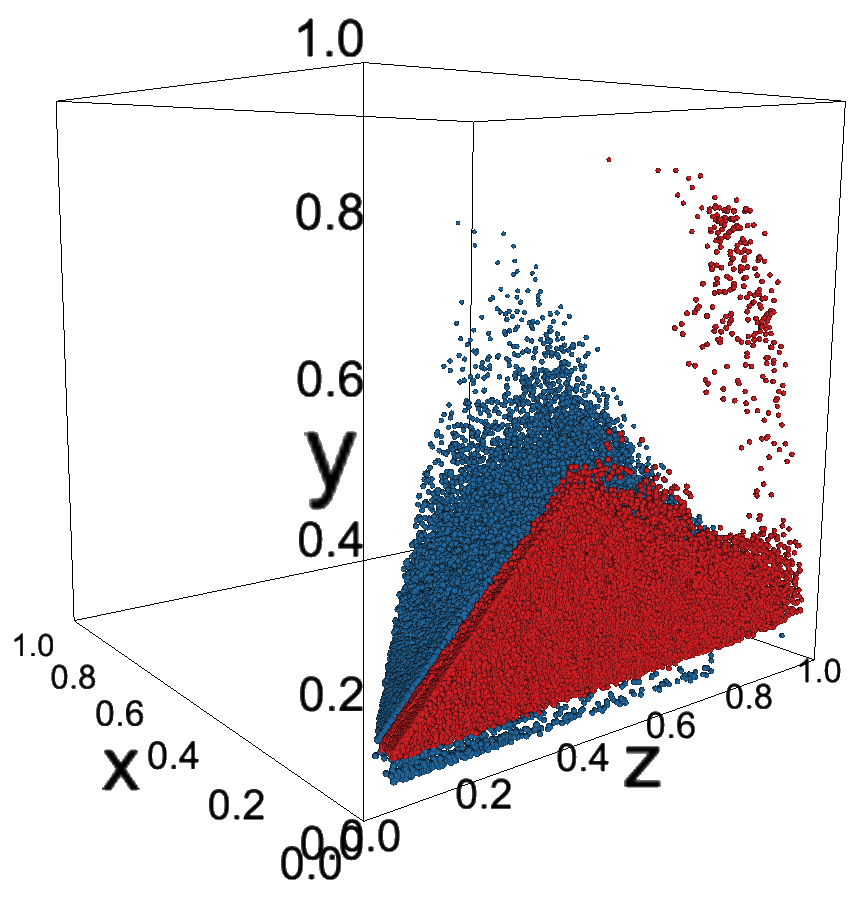
\includegraphics[draft=false, width=0.30\textwidth]{figures/quarks/leptons_high_g_vs_low_1.png}}}%
  \subfloat{{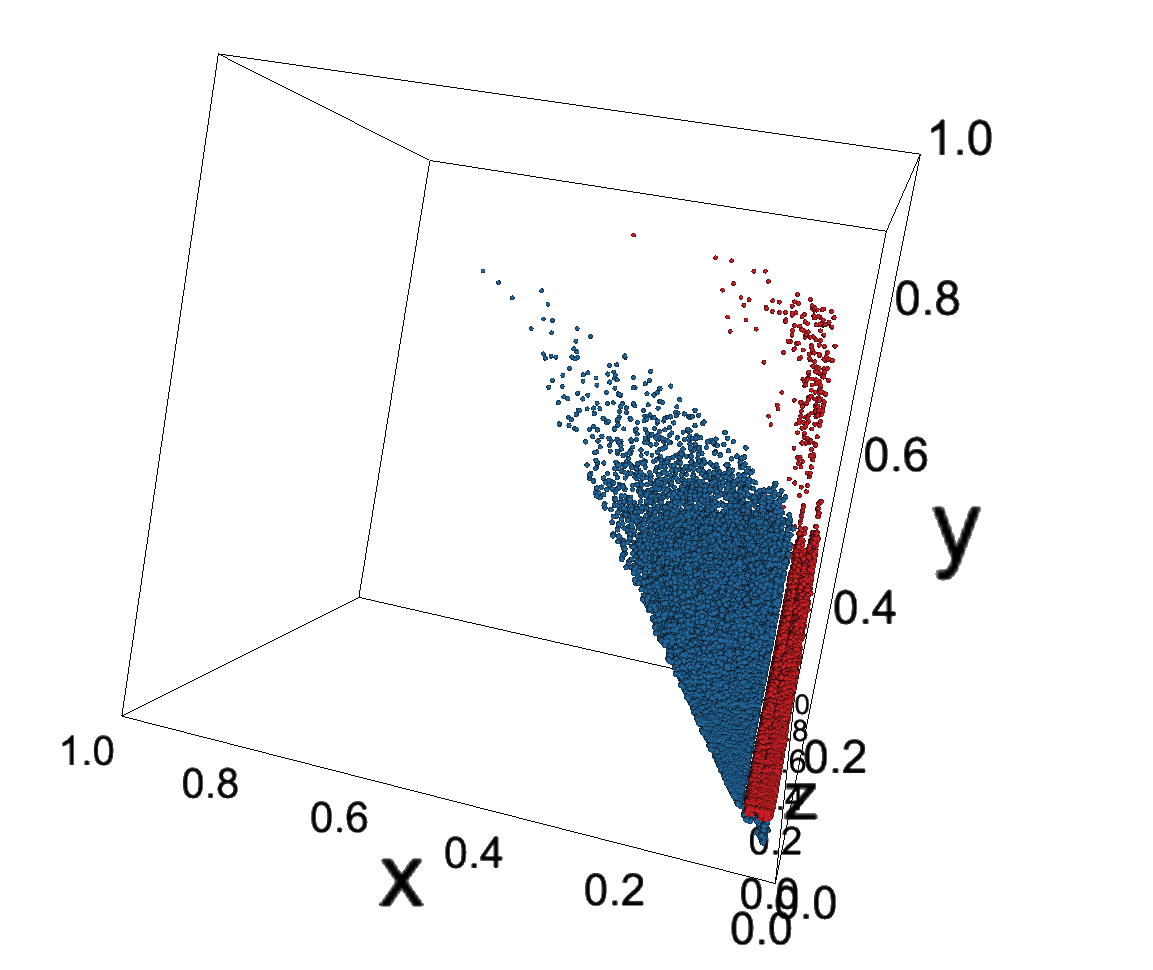
\includegraphics[draft=false, width=0.35\textwidth]{figures/quarks/leptons_high_g_vs_low_3.png}}}%
  \subfloat{{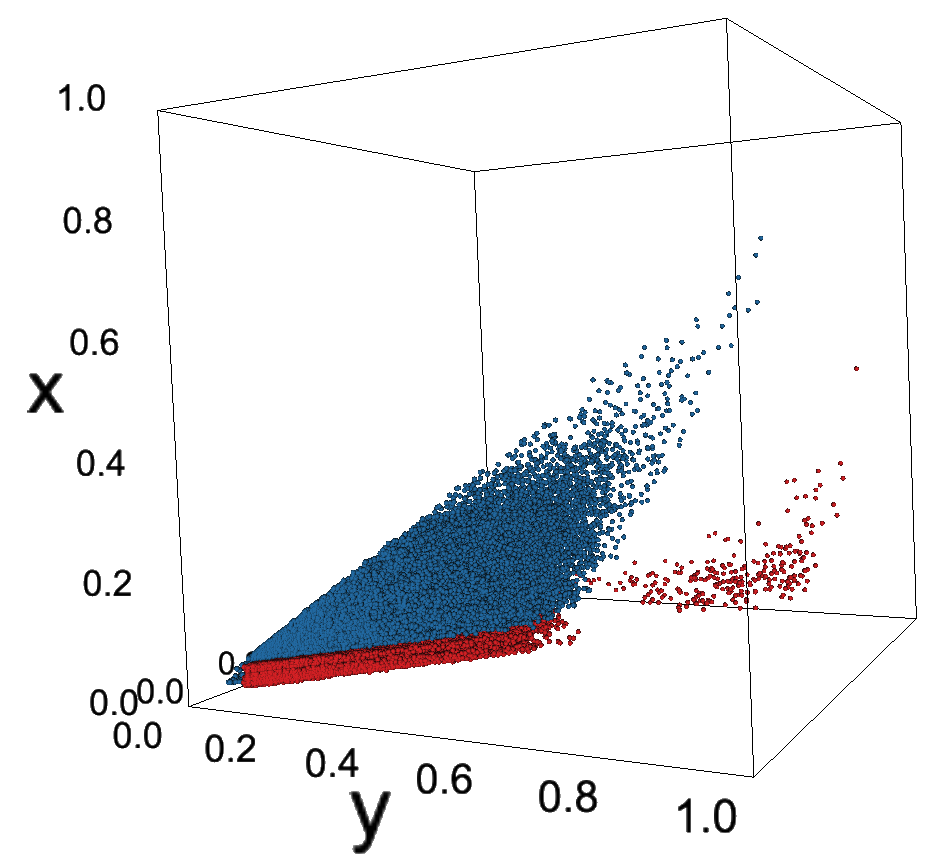
\includegraphics[draft=false, width=0.34\textwidth]{figures/quarks/leptons_high_g_vs_low_2.png}}}%
  \vspace{2mm}
  \caption[3D Scatter Plot of $\beta_\mathrm{tag}$\=/Values for High and Low $\gamma_\mathrm{tag}$ $l$\=/Quark Events]{
    3D scatter plot of $\beta_\mathrm{tag}$\=/values for high and low $\gamma_\mathrm{tag}$ $l$\=/quark events. Here the $x$\=/axis is the lowest $b$\=/tag, the $y$\=/axis
  the middle, and the $z$\=/axis the highest. Here the \textcolor{red}{high\=/$\gamma_\mathrm{tag}$ $l$\=/quark events} are plotted in red and the \textcolor{blue}{low ones} in blue.}
  \label{fig:q:gtag_scores_3j_l_quarks_3d}%
\end{figure*}

\vspace{-5mm}
\section[g-Tagging Efficiency]{$g$\=/Tagging Efficiency}
\label{sec:q:g_tagging_effiency}

These efficiencies are only possible to measure for MC-generated data as the truth labels are required. The Tag-Tag-Probe (TTP) method in \autoref{sec:q:b_tagging_effiency} is not possible for whole events as every event is completely independent of the other and thus one event cannot work as a tag for another event. We can, however, construct a pseudo $g$\=/tagging efficiency based on the $b$\=/tagging efficiencies. This efficiency will be computed by looking at 3-jet events with two jets with a high $b$\=/tag and one jet with a low $b$\=/tag, i.e. events where two jets has $0.9 < \beta_\mathrm{tag}$ and one jet has $\beta_\mathrm{tag} < 0.4$. This indicates a $b\bar{b}g$ event where all of the jets have been correctly identified by the $b$\=/tagging algorithm. The pseudo efficiency $\varepsilon_{b\bar{b}g}$ is then defined as:
\begin{equation}
  \varepsilon_{b\bar{b}g} = \varepsilon_b^{b\dash\mathrm{sig}}\left( b \right) \cdot \varepsilon_b^{b\dash\mathrm{sig}}\left(\bar{b}\right) \cdot \varepsilon_g^{g\dash\mathrm{sig}}\left(g\right).
\end{equation}
This is only a pseudo efficiency since this number is based on the jets in the event and not the event itself, however, by plotting it as a function of an event variable and comparing MC to Data, we can gauge the validity of the $g$\=/tagging algorithm. The first of the event variables used is the $g$\=/tag of the event $\gamma_\mathrm{tag}$, see Figure~\ref{fig:q:effiency_btag_bbg_gtag}. Here the pseudo efficiency is plotted as a function of $\gamma_\mathrm{tag}$ for Data and MC together with the counts in each bin and the ratio between $\varepsilon_{b\bar{b}g}$ for Data and MC is plotted below. At low values of $\gamma_\mathrm{tag}$ the uncertainties dominate due to low statistics, however, at higher $\gamma_\mathrm{tag}$ $\varepsilon_{b\bar{b}g}$ plateaus until very high values of $\gamma_\mathrm{tag}$ where it increases again. The important thing to note in this figure is the high agreement between Data and MC which converges to (almost) \num{1} at high $\gamma_\mathrm{tag}$\=/values. This is an important indication of the 3-jet $g$-tagging model working.

\begin{figure}[h!]
  \centerfloat
  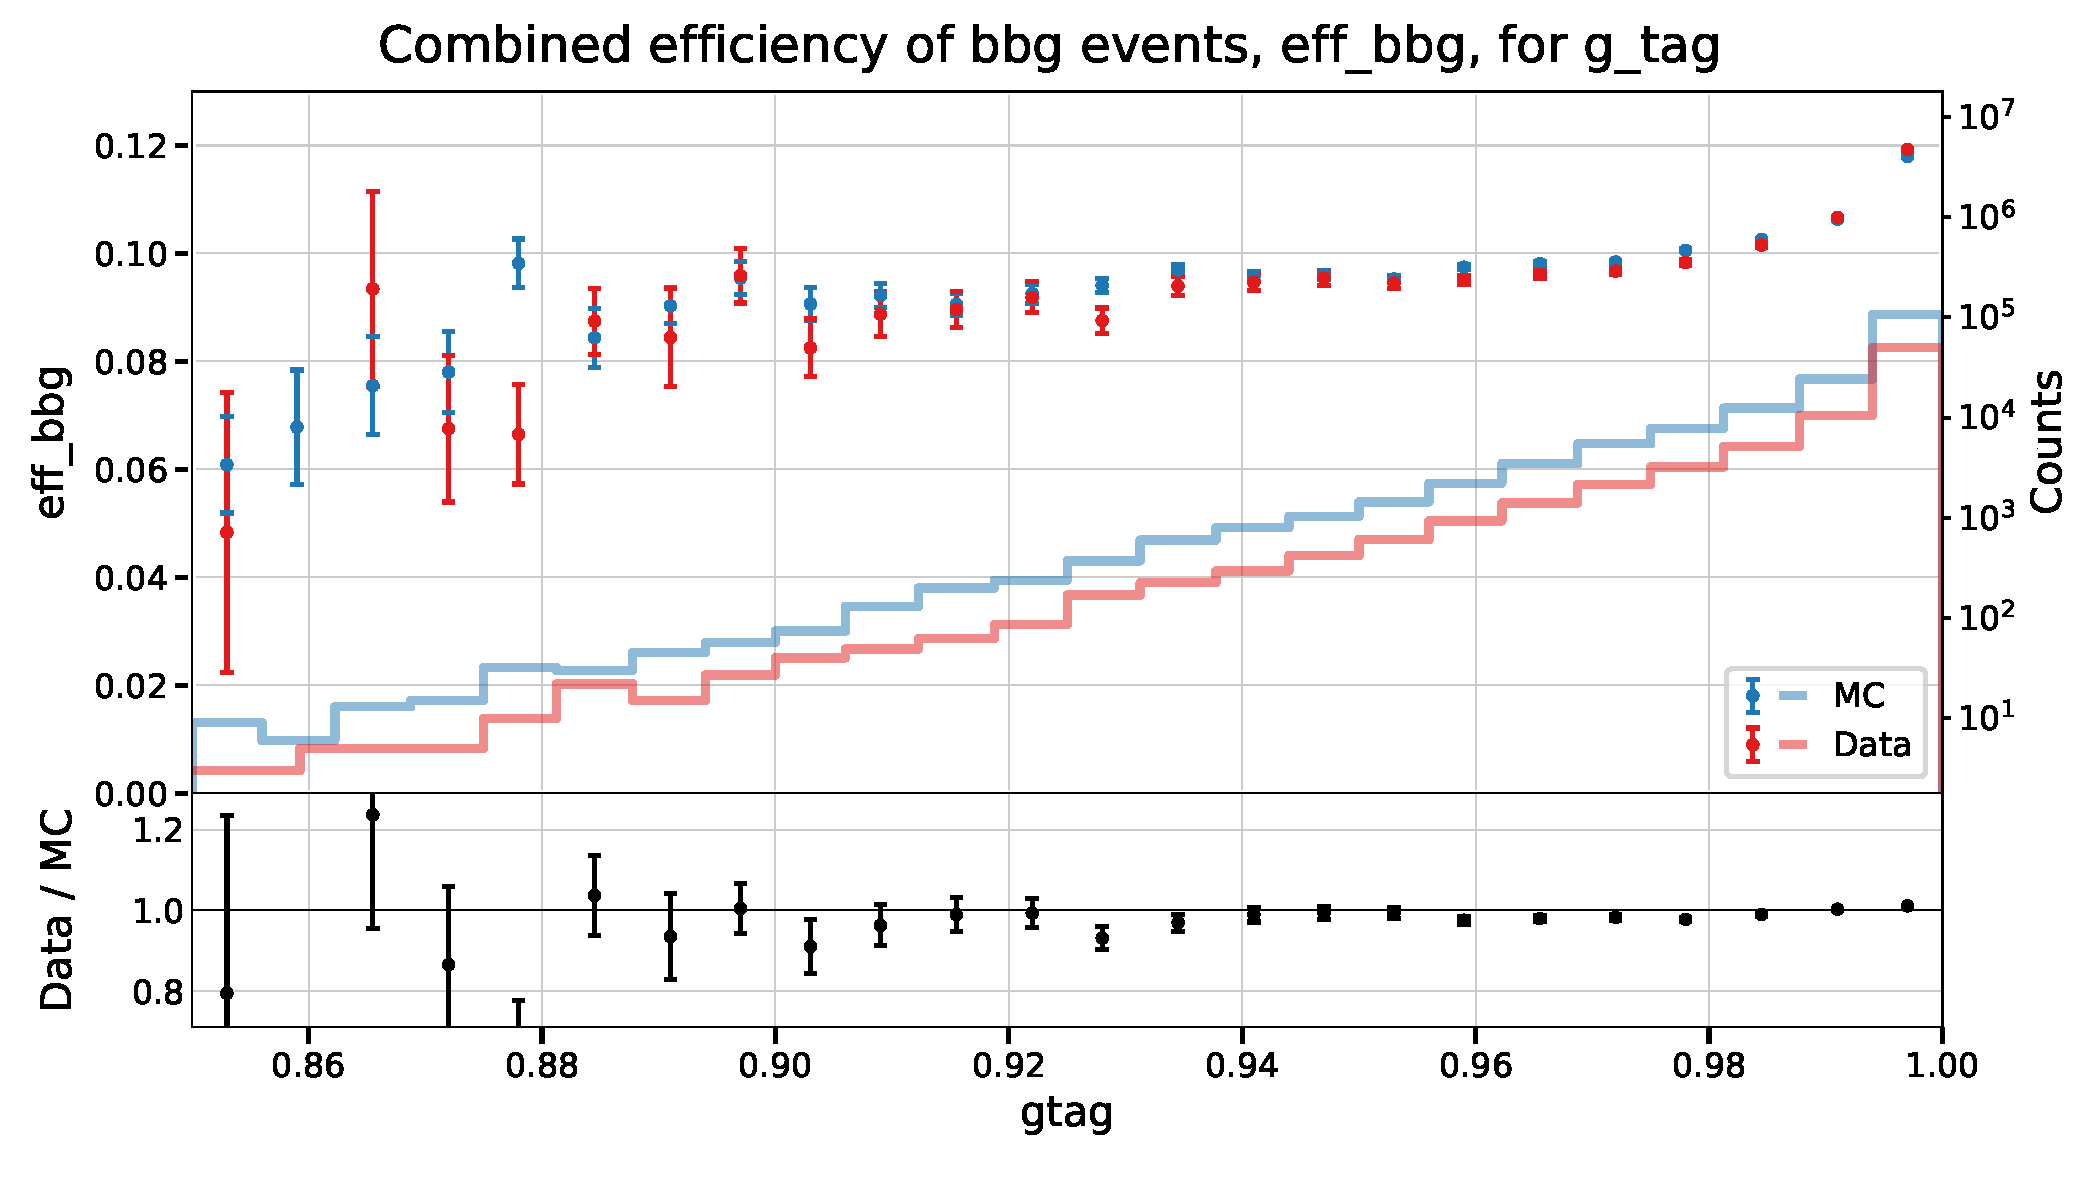
\includegraphics[width=1.1\textwidth, trim=10 20 5 40, clip]{figures/quarks/eff_bbg_gtag-down_sample=1.00-ML_vars=vertex-selection=b-ejet_min=4-n_iter_RS_lgb=99-n_iter_RS_xgb=9-cdot_cut=0.90-version=19.pdf}
  \caption[$g$\=/Tagging Pseudo Efficiency for $b\bar{b}g$\=/Events as a Function of $g$\=/Tag]
          {Pseudo efficiency of the $g$\=/tags for $b\bar{b}g$ 3-jet events as a function of the event's $g$\=/tag $\gamma_\mathrm{tag}$. In the top plot the pseudo efficiency $\varepsilon_{b\bar{b}g}$ is shown for \textcolor{blue}{MC} in blue and \textcolor{red}{Data} in red where the counts in each bin can be read on right $y$\=/axis. In the bottom plot the ratio between Data and MC is shown. The pseudo efficiency is measured by finding $b\bar{b}g$\=/events where $\beta_b > 0.9$, $\beta_{\bar{b}}>0.9$, and $\beta_g < 0.4$. and then calculating  $\varepsilon_{b\bar{b}g} = \varepsilon_b^{b\dash\mathrm{sig}} \cdot \varepsilon_{\bar{b}}^{b\dash\mathrm{sig}} \cdot  \varepsilon_g^{g\dash\mathrm{sig}} $. } 
  \label{fig:q:effiency_btag_bbg_gtag}
\end{figure}

Another event variable to look at is the mean of the two invariant masses $m_{bg}$ and $m_{\bar{b}g}$. The invariant mass between two quantities\sidenote{When measured in natural units.} is:
\begin{equation}
  m_{12} = \sqrt{\left(E_1 + E_2\right)^2 - \norm{\vec{p}_1 + \vec{p}_2}^2 },
\end{equation} 
where $E_i$ is the energy of the $i^\mathrm{th}$ quantity and $\vec{p}_i$ its momentum. The invariant masses between all three jets $m_{b\bar{b}g}$, which otherwise might have been the first intuition to use as the event variable, is non-informative (in this context) since this is just the total event energy which is kept (approximately) constant at $\sim \SI{91}{\GeV}$.

The pseudo efficiency is plotted as a function of the  mean of $m_{bg}$ and $m_{\bar{b}g}$ in Figure~\ref{fig:q:effiency_btag_bbg_m_mean}. Here the overall correspondence between Data and MC is lower than in Figure~\ref{fig:q:effiency_btag_bbg_gtag}, especially for high values of the mean invariant mass. That the ratio is close to \num{1} for most of the data (from \SI{20}{\GeV} to \SI{50}{\GeV}) is a good sign, whereas the tails indicate the model is biased here which could be corrected for with correction factors, however, this would increase the systematic uncertainties. 

\begin{figure}[h!]
  \centerfloat
  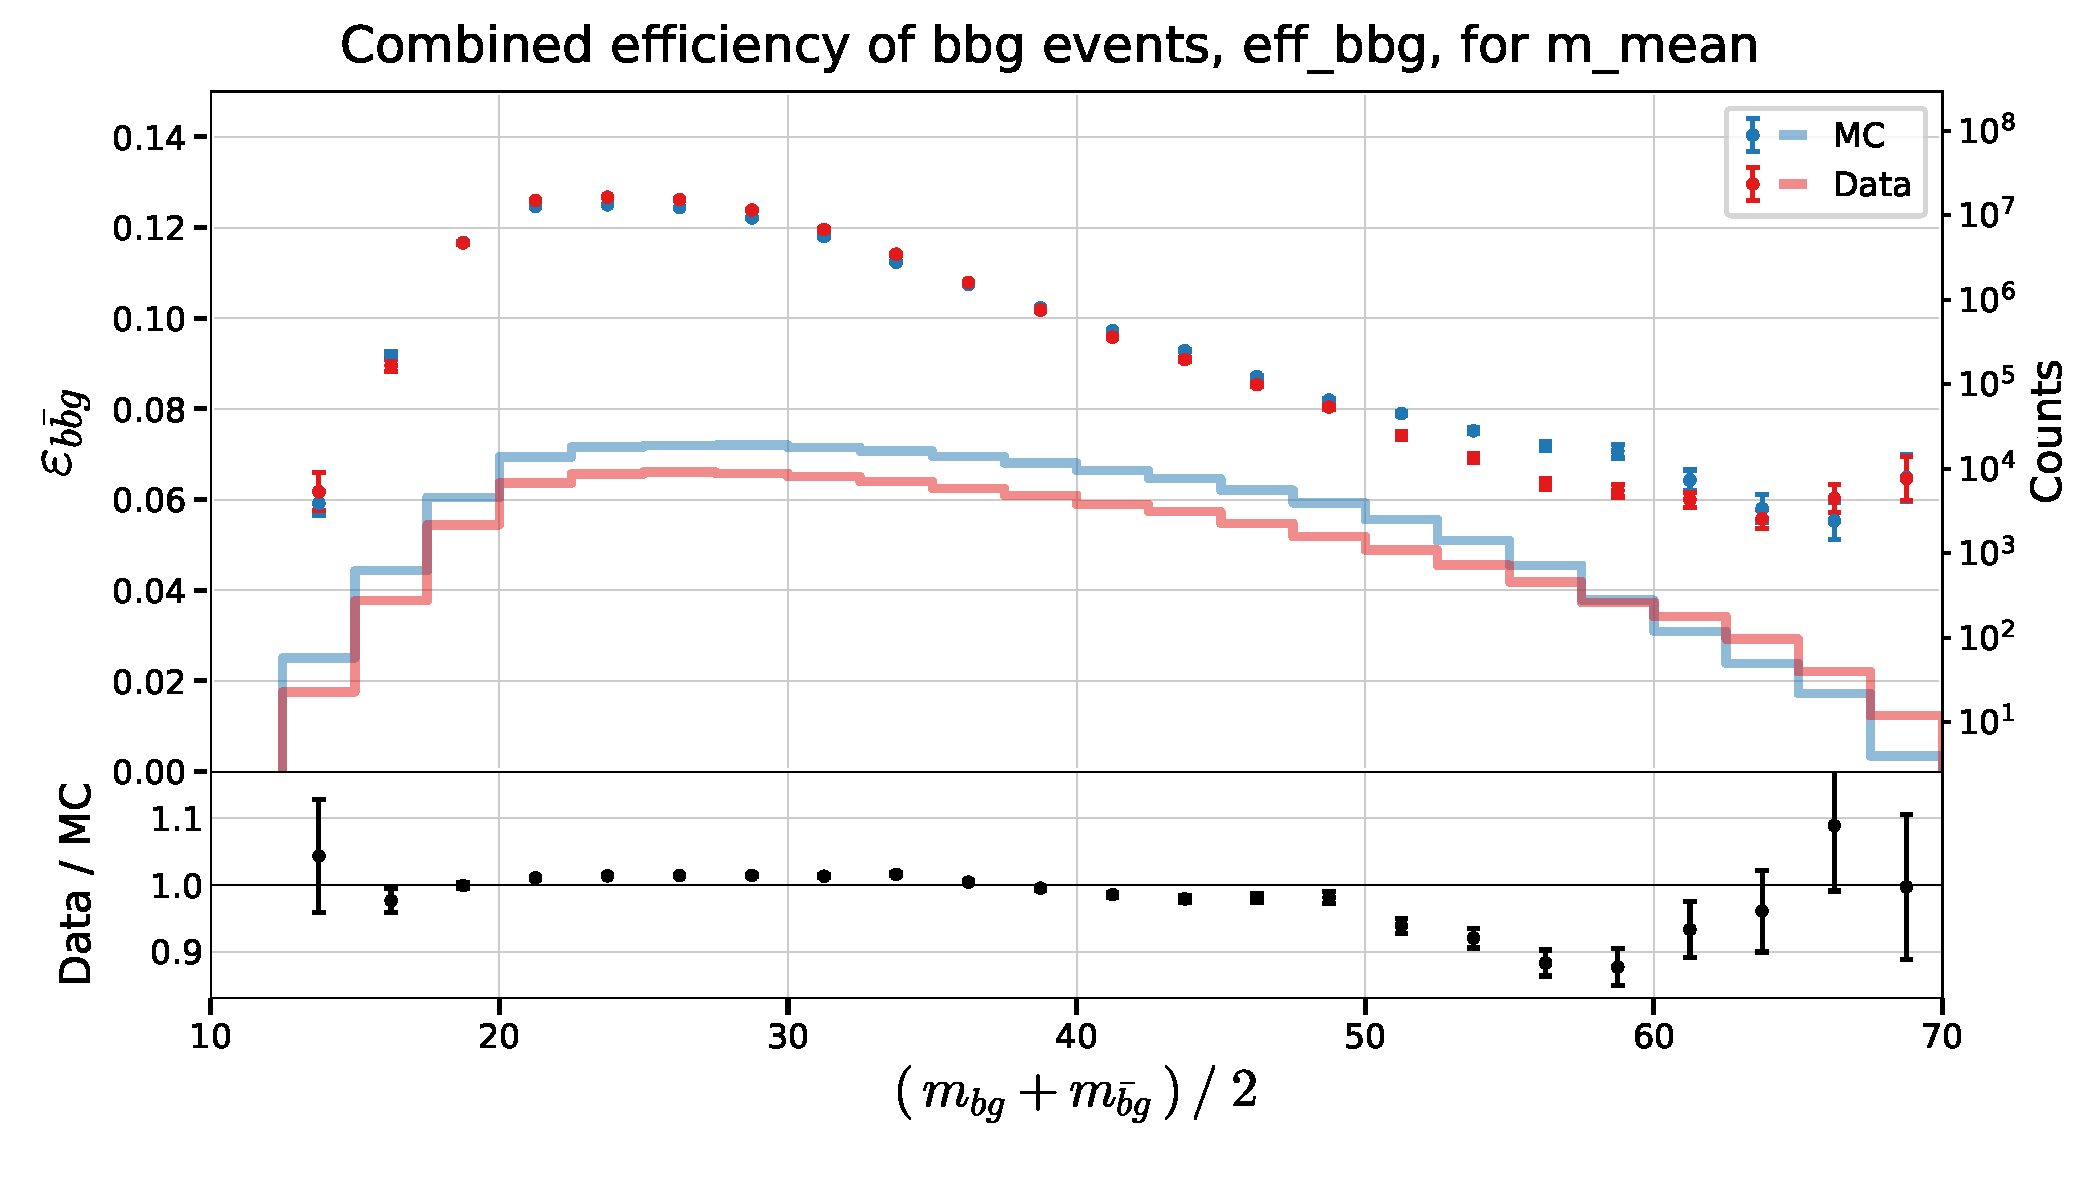
\includegraphics[width=1.1\textwidth, trim=10 20 5 40, clip]{figures/quarks/eff_bbg_m_mean-down_sample=1.00-ML_vars=vertex-selection=b-ejet_min=4-n_iter_RS_lgb=99-n_iter_RS_xgb=9-cdot_cut=0.90-version=19.pdf}
  \caption[$g$\=/Tagging Pseudo Efficiency for $b\bar{b}g$\=/Events as a Function of The Mean Invariant Mass]
          {Pseudo efficiency of the $g$\=/tags for $b\bar{b}g$ 3-jet events as a function of the mean of the two invariant masses $m_{bg}$ and $m_{\bar{b}g}$ in the event. In the top plot the pseudo efficiency $\varepsilon_{b\bar{b}g}$ is shown for \textcolor{blue}{MC} in blue and \textcolor{red}{Data} in red where the counts in each bin can be read on right $y$\=/axis. In the bottom plot the ratio between Data and MC is shown.} 
  \label{fig:q:effiency_btag_bbg_m_mean}
\end{figure}

These two figures strengthens the claim that the trained $b$-tagging and $g$-tagging models provide un-biased models that not only work in Data but also in MC. 

\section{Generalized Angularities in 3-jet events}
\label{sec:q:generalized_angularities_3j}

To measure how gluon jet hadronizes, i.e. their jet distributions, number of tracks, etc., the \emph{generalized angularities} provide an overall framework for doing so. The generalized angularities is a two-parameter family of variables depending on the angular weighting $\beta \leq 0$ and an energy weighting factor $\kappa \leq 0$:
\begin{equation}
  \lambda_\beta^\kappa = \sum_{i \in \mathrm{jet}} z_i^\kappa \theta_i^\beta,
\end{equation}
where $z_i \equiv E_i / E_\mathrm{jet}$ is the momentum fraction, i.e. $0 \leq z_i \leq 1$, $\theta_i \equiv \Omega_i / R$ is the normalized angle with respect to the jet axis where $R$ is the jet radius such that $0 \leq \theta_i \leq 1$, and $i$ runs over all the jet constituents \citep{grasSystematicsQuarkGluon2017,larkoskiGainingMutualInformation2014}. Different values of ($\beta, \kappa$) probe different parts of the (gluon) jet fragmentation phase space. I will limit the analysis to the five sets of ($\beta, \kappa$)-values shown in Figure~\ref{fig:q:LHA}, where each of the sets of variables are related to the following aspects:

\begin{marginfigure}[5.5cm]
  \centerfloat
  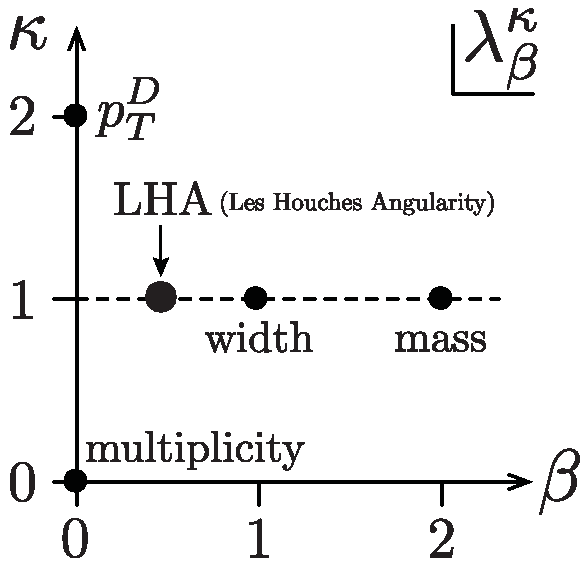
\includegraphics[width=0.9\textwidth]{figures/LHA/LHA.pdf}
  \caption[Generalized Angularities]
          {Generalized angularities. Adapted from \citet{larkoskiGainingMutualInformation2014}. } 
  \label{fig:q:LHA}
\end{marginfigure}

\begin{enumerate}[leftmargin=*,labelindent=16pt]
  \item[($\beta, \kappa$)\phantom{:}]
  \item[($0, 0$):] Hadron Multiplicity.
  \item[($0, 2$):] Transverse Momentum Distribution $p_T^D$: \\
  $\lambda_0^2=\sum z_i^2 \equiv \left(p_T^D \right)^2$ \autocite{cmscollaborationSearchHiggsBoson2012}.
  \item[($\frac{1}{2} , 1$):] Les Houches Angularity (LHA) \autocite{thalerReportHouchesQuark}.
  \item[($1, 1$):] Width or broadening \citep{cataniJetBroadeningMeasures1992a}.
  \item[($2, 1$):] Mass.
\end{enumerate}

We will look at the generalized angularity distributions for gluons in 3-jet events. We do so by using the $g$-tag from the $g$-tagging model to select events with a high $g$-tag and then select the jet in the event with the lowest of the $b$-tags since this jet is expected to be the gluon jet. From the plot in Figure~\ref{fig:q:gtag_scores_3j_sig_bkg}, the $\gamma_\mathrm{tag}$ cut off threshold is set to $\gamma_\mathrm{cutoff} = 0.9$ for 3-jet events. This cut corresponds to selecting \num{340476} events in MC as gluon events with a signal efficiency of $\varepsilon_g^{3\dash\mathrm{jet}} = \SI{19.68}{\percent}$ and a signal purity of $\rho_g^{3\dash\mathrm{jet}}=\SI{98.77}{\percent}$. Here a gluon event is defined as an event with a $0.9 < \gamma_\mathrm{tag}$. 

The distribution of $\lambda_0^2$, i.e. $(\beta, \kappa)=(0,2)$, related to the transverse momentum distribution, in gluon events is seen in Figure~\ref{fig:q:generalized_angularities_cha_lambda_0_2_nonappendix}. Here the distribution of $\lambda_0^2$ is shown for MC Truth (actual gluons jets using truth-label), MC selected (gluons jets selected using the $g$-tag) and Data (gluons jets selected using the $g$-tag). The generalized angularities are computed for both charged jets and neutral clusters, where this figure shows the distribution of $\lambda_0^2$ for charged jets. The MC Selected has been scaled to Data according to the fraction of the number of events in each: $w_\mathrm{MC} = N_\mathrm{Data} / N_\mathrm{MC}$. The MC Truth has been scaled with the same weight multiplied with the gluon efficiency $w_\mathrm{MC \dash Truth} = w_\mathrm{MC} \cdot \varepsilon_g^{3\dash\mathrm{jet}}$. The $\lambda_\beta^\kappa=0$ values has been removed before plotting for all sets of values of $(\beta, \kappa)$. 

In Figure~\ref{fig:q:generalized_angularities_cha_lambda_0_2_nonappendix} it is seen how MC Truth and Data does not match perfectly well which indicates that this is not the perfect method, however, that MC Selected and Data distributions matches each other quite well indicates that the model is equally biased for both MC and Data. 
The errorbars in the ratio plot are fitted with both a constant ${f(x)=b}$ and a straight line $f(x)=ax+b$ with the fit results shown as text in the plot. In the text box \code{DOF} is the number of degrees of freedom and \code{P} is the $\chi^2$-probability\sidenote{ $P(\chi^2; N_\mathrm{DOF}) = \int_{\chi^2}^\infty f_{\chi^2}(x; N_\mathrm{DOF}) \mathop{dx}$, where $f_{\chi^2}(x; N_\mathrm{DOF})$ is the $\chi^2$ distribution with $N_\mathrm{DOF}$ degrees of freedom.}. I compute the systematic error $\sigma_\mathrm{sys}$ that would have to be added in quadrature to the standard deviation, $\sigma \rightarrow \sqrt{\sigma^2 + \sigma_\mathrm{sys}^2}$, such that the $\chi^2$-probability would be \SI{50}{\percent}. I do this using Brent's method \autocite{Brent:113464} and the systematic error is written as \code{sigma_sys} in the figure. 

\begin{figure}[h!]
  \centerfloat
  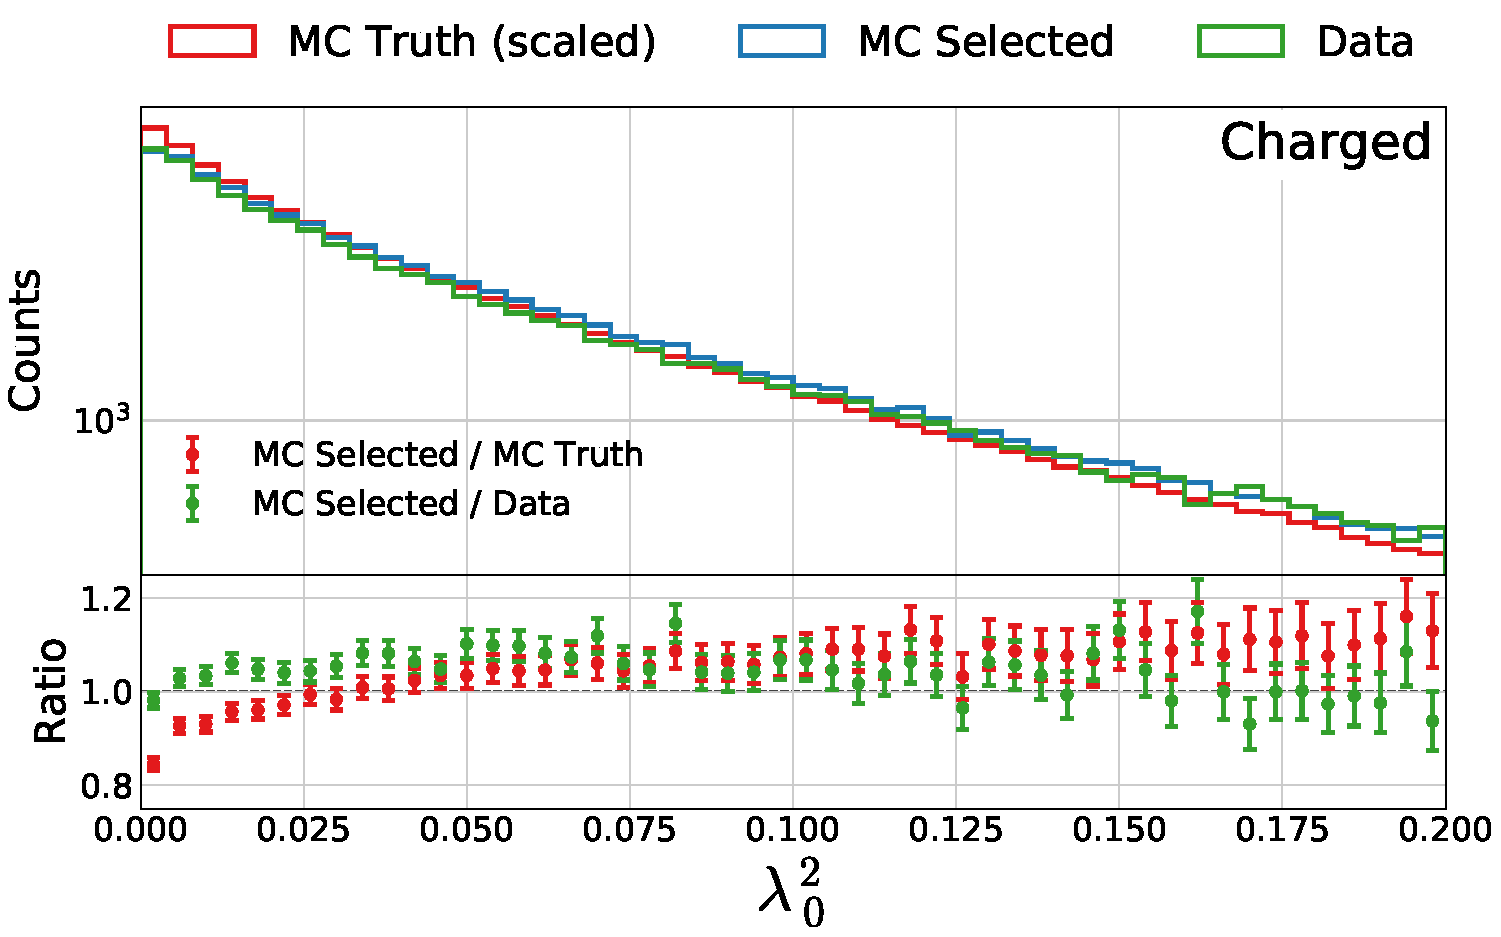
\includegraphics[width=0.99\textwidth, trim=0 0 0 0, clip, page=1]{figures/quarks/generalized_angularities_cha-down_sample=1.00-ML_vars=vertex-selection=b-ejet_min=4-n_iter_RS_lgb=99-n_iter_RS_xgb=9-cdot_cut=0.90-version=19.pdf}
  \caption[Generalized Angularities for Charged Gluons Jets in 3-Jet Events: $\lambda_0^2$]
          {Distribution of the generalized angularity $\lambda_0^2$ for charged gluons jets in 3-jet events: $\lambda_0^2$. The distributions for \textcolor{red}{MC Truth} is shown in red, \textcolor{blue}{MC Truth} in blue, and \textcolor{green}{Data} in green in the top plot and in the bottom plot the ratio between \textcolor{red}{MC Selected and MC Truth} is shown in red and between \textcolor{green}{MC Selected and Data} in green. }
  \label{fig:q:generalized_angularities_cha_lambda_0_2_nonappendix}
\end{figure}
\vspace{-3mm} 

The rest of the plots can be seen in Figure~\ref{fig:q:generalized_angularities_cha_lambda_0_2}--\ref{fig:q:generalized_angularities_neu_lambda_0_0}. For the charged tracks it can be seen that the first few bins generally has ratios just below \num{1} with a upwards trend until around the middle of the $\lambda$ range and then it decreases again (and the uncertainties increases with lower and lower statistics). The discrepancy between MC selected and Data is larger for the neutral clusters, which are also less well-defined than the charged jets (at the energies used at LEP), and with the same trend as for the charged jets. 

These trends are quantified in by the fits to the ratio plots. For $\lambda_0^2$, Figure~\ref{fig:q:generalized_angularities_cha_lambda_0_2_nonappendix} above, we see that a constant fit does a reasonable job with a $P_\chi^2=\SI{3.9}{\percent}$. The small decrease in $\chi^2$ value, $\chi^2 = 67.76$ for the constant fit but only \num{67.65} for the linear fit, is attributed to the linear fit being a more advanced fit (more fit parameters). In this case the difference would be expected to be $\Delta \chi^2 \sim 1$ due to difference in the number of fit parameters being \num{1}, which is also what is seen. As such, the systematic error will be based on the constant fit here $\sigma_\mathrm{sys}(\lambda_0^2)=\SI{2.0}{\percent}$. 

\begin{margintable}[-6cm]
  \centerfloat
  \begin{tabular}{@{}rrc@{}}
  {}             & $\sigma_\mathrm{sys}$ & $f(x)$ \\ \addlinespace[0.1em] \midrule \addlinespace[0.2em]
  $\lambda_0^2$        & $\SI{2.0}{\percent}$  & $b$ \\ \addlinespace[0.2em]
  $\lambda^1_{1/2}$    & $\SI{2.1}{\percent}$  & $b$ \\ \addlinespace[0.2em]
  $\lambda_1^1$        & $\SI{1.1}{\percent}$  & $ax+b$ \\ \addlinespace[0.2em]
  $\lambda_2^1$        & $\SI{0.4}{\percent}$  & $ax+b$ \\ \addlinespace[0.2em]
  $\lambda_0^0$        & $\SI{7.5}{\percent}$  & $b$ \\ \addlinespace[0.2em]
  \end{tabular}
  \vspace{3mm}
  \caption[Generalized Angularities Systematic Errors, Charged Tracks]{\label{tab:q:generalized_angularities_systematic_errors_charged}Systematic errors for the generalized angularities for charged tracks.  The last column, $f(x)$, denotes which fit the systematic error is based on.}
\end{margintable}

\begin{margintable}
  \centerfloat
  \begin{tabular}{@{}rrc@{}}
  {}             & $\sigma_\mathrm{sys}$ & $f(x)$ \\ \addlinespace[0.1em] \midrule \addlinespace[0.2em]
  $\lambda_0^2$        & $\SI{4.2}{\percent}$  & $ax+b$ \\ \addlinespace[0.2em]
  $\lambda_{1/2}^1$    & $\SI{4.2}{\percent}$  & $ax+b$ \\ \addlinespace[0.2em]
  $\lambda_1^1$        & $\SI{3.9}{\percent}$  & $ax+b$ \\ \addlinespace[0.2em]
  $\lambda_2^1$        & $\SI{1.6}{\percent}$  & $ax+b$ \\ \addlinespace[0.2em]
  $\lambda_0^0$        & $\SI{2.0}{\percent}$  & $b$ \\ \addlinespace[0.2em]
  \end{tabular}
  \vspace{3mm}
  \caption[Generalized Angularities Systematic Errors, Neutral Clusters]{\label{tab:q:generalized_angularities_systematic_errors_neutral}Systematic errors for the generalized angularities for neutral clusters.  The last column, $f(x)$, denotes which fit the systematic error is based on.}
\end{margintable}

In general there is a $\sim \SI{4}{\percent}$ constant offset for the charged tracks, which is easy to correct for. For the neutral clusters it is seen to be a lot higher at $\sim \SI{15}{\percent}$. For charged tracks the systematic error is around $\sim \SI{2}{\percent}$ for most of the generalized angularities, while it is around $\sim \SI{4}{\percent}$ for the neutral clusters. A summary of all the systematic errors for the charged tracks can be seen in Table~\ref{tab:q:generalized_angularities_systematic_errors_charged} and in Table~\ref{tab:q:generalized_angularities_systematic_errors_neutral} for the neutral clusters. Overall, the figures show a reasonable good correspondence between MC selected and Data for the generalized angularities.  

\section{Gluon splitting}
\label{sec:q:gluon_splitting_4j}

In addition to measuring how the gluon jets hadronizes, we are also interested in measuring how they split: $g \rightarrow gg$. We do so by looking at 4-jet events with high $g$-tag values and then identify the two gluon jets (the ones with the lowest $b$-tag values). From Figure \ref{fig:q:gtag_scores_4j_sig_bkg}, the $\gamma_\mathrm{tag}$ cut off threshold is set to $\gamma_\mathrm{cutoff} = 0.8$ for 4-jet events. This corresponds to selecting \num{41117} events in MC as gluon events with a signal efficiency of $\varepsilon_g^{4\dash\mathrm{jet}} = \SI{23.30}{\percent}$ and a signal purity of $\rho_g^{4\dash\mathrm{jet}}=\SI{92.67}{\percent}$. 
\marginnote[-1cm]{Note that the number of selected events in the 4-jet case is much lower than in the 3-jet case and that the signal purity is lower as well, $\rho_g^{3\dash\mathrm{jet}}=\SI{98.77}{\percent}$ vs. $\rho_g^{4\dash\mathrm{jet}}=\SI{92.67}{\percent}$, at the selected cut value.}
% The variables related to measuring the gluon splitting will be introduced in \autoref{subsec:q:gluon_splitting_variables} and their efficiencies in MC will be computed in \autoref{subsec:q:gluon_splitting_efficiency}. The method will be tested with a closure test in \autoref{subsec:q:gluon_splitting_closure} and the results shown in \autoref{subsec:q:gluon_splitting_results}.

\subsection{Variables}
\label{subsec:q:gluon_splitting_variables}
The variables we use to measure the gluon splitting are each meant to probe different, smaller parts of the phase space. It is difficult to parametrize the basis of this phase space, but in discussion with one of the authors of the MC simulator Pythia \autocite{sjostrandIntroductionPYTHIA2015}, Peter Skands, the first dimension of the phase space will be the energy asymmetry. The energy asymmetry describes how the two gluons share their available energy between them; do they share it equally or does one of them get the majority of it? The second dimension is the resolution scale which probes the hardness of the gluons by looking at their invariant mass and the angle between the their jets. The third axis is the azimuthal angle which measures the rotational distribution of the gluons compared to the quarks. In addition to these, some extra variables were proposed by Peter Skands \autocite{skandsPeterSkands2019}. These \q{Peter Skands}\=/variables are aimed at other probing other interesting areas of the phase space. 
 
The gluon splitting variables are variables where current MC generators, such as Pythia, and Data show some discrepancies. Better measurements of these variables might lead to new theoretical insights that can reduce these discrepancies. The gluon splitting variables are:

\begin{enumerate}[leftmargin=*,labelindent=40pt]
  
  % \item[\textbf{Energy Assymetri}:]
  \item[] \textbf{Energy Asymmetry:} 
  \item[$E_\mathrm{diff}$:] The relative difference in energy between the gluon jet with the highest and lowest energy: $E_\mathrm{diff} = \frac{E_\mathrm{max}-E_\mathrm{min}}{E_\mathrm{max}+E_\mathrm{min}}$.
  \item[$E_{\mathrm{rel}_\mathrm{min}}$:] The relative energy of the gluon jet with the lowest energy and the sum: $E_{\mathrm{rel}_\mathrm{min}} = \frac{E_\mathrm{min}}{E_\mathrm{max}+E_\mathrm{min}}$.
  \item[$E_\mathrm{rel}$:] The relative energy of the gluon jet with the lowest energy and the highest energy: $E_\mathrm{rel} = \frac{E_\mathrm{min}}{E_\mathrm{max}}$.

  \item[] \textbf{Resolution Scale:}
  \item[$\Delta_\theta$:] The angle between the two gluon jets.   
  \item[$m_{gg}$:] The invariant mass of the two gluon jets.

  \item[] \textbf{Azimuthal Angle} 
  \item[$\phi_\mathrm{\parallel}$:]  The angle between the plane spanned by the two $b$-jets and the plane spanned by the two gluon jets. This is the same angle as the angle between the $b$-jet cross product $\vec{p}_{b_1} \times \vec{p}_{b_2}$ and the gluon-jet cross product $\vec{p}_{g_1} \times \vec{p}_{g_2}$ where $\vec{p}$ is the jet momentum.

  \item[] \textbf{Peter Skands:} 
  \item[$\ln \left( k_t^2 / m_\mathrm{vis}^2 \right)$:] Logarithm of the ratio between the $k_t$ value, see equation \eqref{eq:q:k_t_definition_kt}, of the two gluon jets and the visible mass of the event.  
  \item[$p^2_{\perp,\mathrm{A}}$:] The $p_perp$ antenna defined as: 
  \begin{fullwidth}
    \begin{flalign}
      p^2_{\perp,\mathrm{A}} = \widetilde{m}_{12}^2 \cdot \min \bigg( \frac{\min \big(\widetilde{m}_{b1}^2, \widetilde{m}_{b2}^2 \big) - m_b^2}{\widetilde{m}_{b12}^2 - m_b^2}, \; \frac{\min \big(\widetilde{m}_{\bar{b}1}^2, \widetilde{m}_{\bar{b}2}^2 \big) - m_b^2}{\widetilde{m}_{\bar{b}12}^2 - m_b^2}  \bigg), &&
    \end{flalign}
  \end{fullwidth}
  where $\widetilde{m}^2 = m^2 \cdot m_Z^2 / m_\mathrm{vis}^2$ and $m_Z$ is the mass of the $Z$ boson.  

  % \item[] \textbf{Jet Clustering} 
  % \item[$R_{gg}^{k_t}$:] The ratio between the $k_t$ distance measure for the gluon jets and the minimum non-$gg$ jets: $R_{gg}^{k_t} \equiv R_{gg}(p=1)$, see equation \eqref{eq:q:kt_CA_distance_measure}.
  % \item[$R_{gg}^\mathrm{CA}$:] Same as above, however for the CA algorithm: $R_{gg}^{CA} \equiv R_{gg}(p=0)$. 
\end{enumerate}

The gluon splitting variables will be analyzed in distinct regions defined by the $k_t$ \citep{cataniLongitudinallyinvariantKtclusteringAlgorithms1993,ellisSuccessiveCombinationJet1993} and Cambridge/Aachen (CA) \citep{dokshitzerBetterJetClustering1997,wobischHadronizationCorrectionsJet1999} jet clustering algorithms for $e^+e^-$ collisions which will first be described. The two algorithms uses the following\sidenote{When using $R=1$ in eq. (9a) in Ref. \autocite{cacciariFastJetUserManual2012}.} \emph{jet distance measure}:
\begin{equation}
  \label{eq:q:kt_CA_distance_measure}
  d_{ij}^2(p) = \min \left(E_i^{2p}, E_j^{2p} \right) \left(\frac{1-\cos \theta_{ij}}{2} \right), 
\end{equation}
where $E$ is the (pseudo)jet energy and $\theta_{ij}$ is the angle between (pseudo)jet $i$ and $j$ \autocite{cacciariFastJetUserManual2012}. For $p=1$ equation \eqref{eq:q:kt_CA_distance_measure} is called the $k_t$ algorithm and the Cambridge/Aachen for $p=0$. Both the $k_t$ and CA algorithms are newer jet clustering algorithms than JADE, see \autoref{sec:hep:jet_clustering}, and their distance measures are also pretty similar to JADE's. The value $d_{ij}(p=1)$ is also known as the $k_t$:
\begin{equation}
  \label{eq:q:k_t_definition_kt}
  k_t = \sqrt{\min \left(E_i^2, E_j^2 \right) \left(\frac{1-\cos \theta_{ij}}{2} \right)}.
\end{equation}

Based on the two algorithms, we define the ratio $R_{gg}$ between the two gluon jets $d^2_{gg}$ and the lowest value of $d^2_{ij}$ not including the two gluon jets:
\begin{equation}
  R_{gg}(p) \equiv \frac{d^2_{gg}(p)}{\min_{(i,j) \neq (g,g)} d^2_{ij}(p)}.
\end{equation} 
We further define $R_{gg}^{k_t} \equiv R_{gg}(p=1)$ and $R_{gg}^{CA} \equiv R_{gg}(p=0)$. 

\begin{marginfigure}[-2cm]
  \centerfloat
  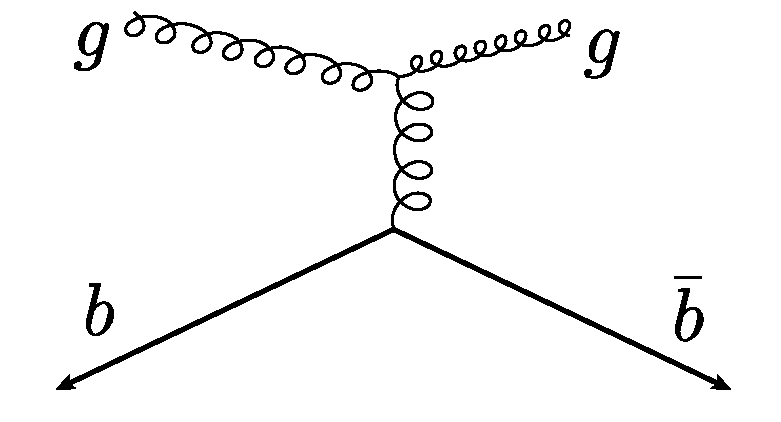
\includegraphics[width=1.1\textwidth]{figures/R_kt_CA/soft_wide_angle.pdf}
  \caption[Soft Wide Angle Gluons in 4-Jet Events]
          {Soft, wide angle gluons in 4-jet events.} 
  \label{fig:q:kt_CA_soft_wide}
\end{marginfigure}


\begin{marginfigure}[1cm]
  \centerfloat
  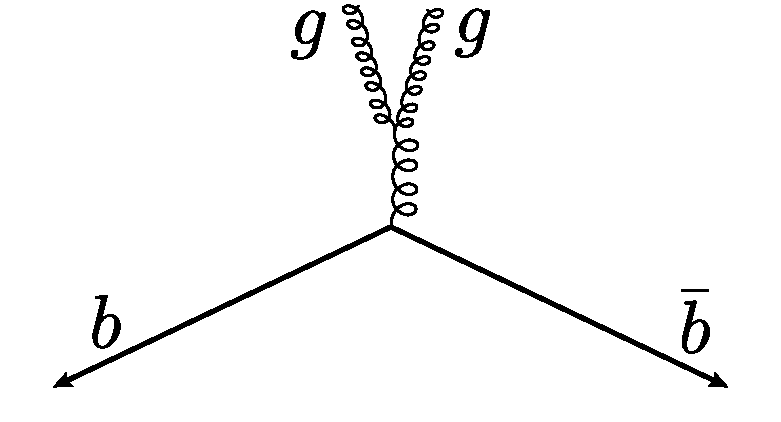
\includegraphics[width=1.1\textwidth]{figures/R_kt_CA/soft_collinear.pdf}
  \caption[Soft Collinear Gluons in 4-Jet Events]
          {Soft, collinear gluons in 4-jet events.} 
  \label{fig:q:kt_CA_soft_collinear}
\end{marginfigure}

\begin{marginfigure}[1cm]
  \centerfloat
  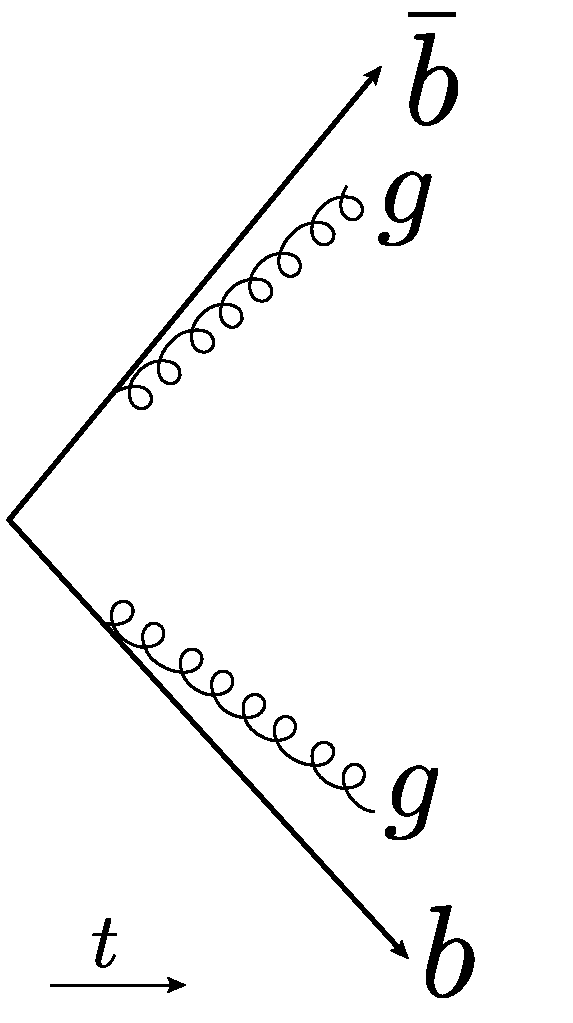
\includegraphics[width=1.1\textwidth]{figures/R_kt_CA/hard_non_g_to_gg.pdf}
  \caption[Hard Non $g\rightarrow gg$ Gluons in 4-Jet Events]
          {Hard, non $g\rightarrow gg$ gluons in 4-jet events.} 
  \label{fig:q:kt_CA_hard_non_g_to_gg}
\end{marginfigure}

Since the CA algorithm is energy-independent and the $k_t$ algorithm is not, they describe different parts of the phase space. One example of this is the case of soft wide gluon jets illustrated in Figure~\ref{fig:q:kt_CA_soft_wide}. Here the two gluon jets are low-energy (soft) jets but with a high angle between them (wide). In this case the $k_t$ algorithm would probably cluster the two gluon jets together but the CA algorithm would not. This means that $R_{gg}^{k_t}$ would be less than \num{1} since the distance measure between the two gluon jets would be the smallest of them all, whereas to $R_{gg}^{CA}$ would be larger than \num{1} since $d_{\bar{b}g} < d_{gg}$. In addition to the soft, wide angle gluon jets, we have the case of soft, collinear gluon jets which the two algorithms agree to cluster together, see Figure~\ref{fig:q:kt_CA_soft_collinear} or the opposite case where the two algorithms both agree on not to cluster the gluon jets together, see Figure~\ref{fig:q:kt_CA_hard_non_g_to_gg}. These figures are just illustrations of how to better understand the $R_{gg}$ phase space.


The variables are computed on an event-by-event basis.
% and their relationship with $\gamma_\mathrm{tag}$ is shown in Figure~\ref{fig:q:gtag_gluon_splitting_variable_E_diff}--\ref{fig:q:gtag_gluon_splitting_variable_pt_antenna}. 
From now on primarily events with with \q{good} $g$-tags, $\gamma_\mathrm{tag} > 0.8$, are used. The efficiency of these signal events are measured in the following subsection. 

\subsection{Efficiencies}
\label{subsec:q:gluon_splitting_efficiency}
It is not possible to take advantage of the Tag-Tag-Probe method for whole events as it was for individual jets in the 3-jet case. As such, we are also unable to estimate the $g$-tagging efficiency in Data of the gluon splitting variables defined in the previous subsection. However, it is still possible to do so for MC using the truth labels. The efficiency $\varepsilon_{gg}^{4\dash\mathrm{jet}}$ for the gluon splitting variable $E_\mathrm{diff}$ is shown in Figure~\ref{fig:q:effiency_gtag_E_diff_non_appendix} for signal and background based on MC Truth. Note that even though the efficiency here is quite low, it is close to constant (as a function of $E_\mathrm{diff}$).

\begin{figure}
  \centerfloat
  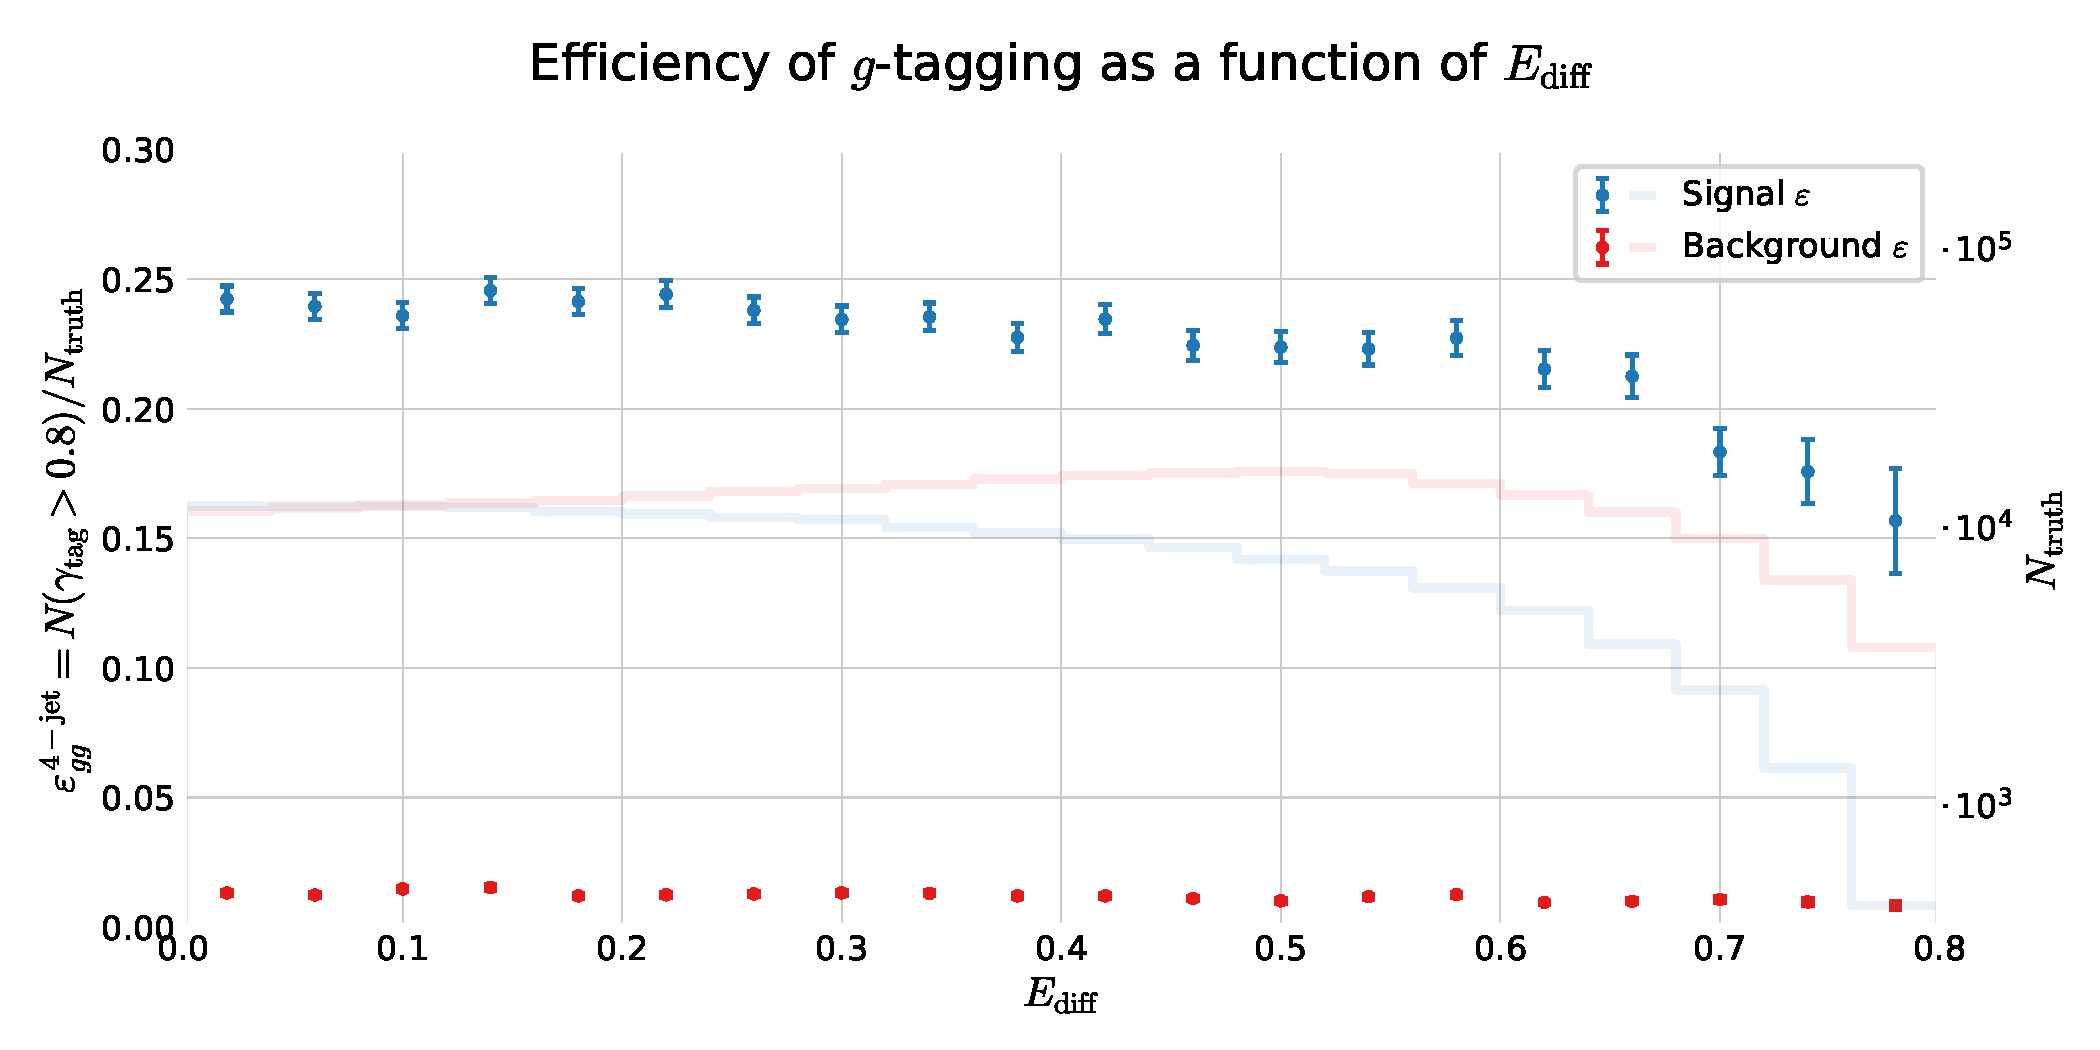
\includegraphics[width=0.95\textwidth, trim=10 10 10 45, clip, page=1]{figures/quarks/efficiency_events-down_sample=1.00-ML_vars=vertex-selection=b-ejet_min=4-n_iter_RS_lgb=99-n_iter_RS_xgb=9-cdot_cut=0.90-version=19-njet=4.pdf}
  \caption[$g$-Tagging Efficiency for 4-Jet Events in MC as a Function of the Normalized Gluon-Gluon Jet Energy Difference Asymmetry $E_\mathrm{diff}$]
          {Efficiency of the $g$-tagging algorithm for 4-jet events as a function of normalized gluon-gluon jet energy difference (asymmetry) $E_\mathrm{diff}$  in MC. The efficiency is measured as the number of events with a $g$-tag higher than 0.8 ($\gamma > 0.8$) out of the total number. The efficiency is plotted for \textcolor{blue}{signal events} according to MC Truth in blue and \textcolor{red}{background events} according to MC Truth in red.
          } 
  \label{fig:q:effiency_gtag_E_diff_non_appendix}
\end{figure}

The plot for the rest of the $g$-tagging efficiencies can be seen in Figure~\ref{fig:q:effiency_gtag_E_diff}--\ref{fig:q:effiency_gtag_pt_antenna}. 

\subsection{Closure Test}
\label{subsec:q:gluon_splitting_closure}

I perform a closure test to validate the $g$-tagging model for the gluon variables in 4-jet events. Closure tests compare the developed method after corrections\sidenote{E.g. Applying the efficiencies found in the previous subsection.} to MC Truth. Any discrepancies can then be investigated and finally the closure test can gauge the systematic uncertainties of the analysis. 

The closure test is based on the distribution of the gluon splitting variables, see \autoref{subsec:q:gluon_splitting_variables}, for events in the signal region or the so-called \emph{sideband region}. The sideband region\sidenote{Also sometimes known as the control region.} is a region close to the signal region where the background is expected to behave approximately similar to the background in the signal region (and likewise for the signal). From Figure \ref{fig:q:gtag_scores_4j_sig_bkg}, the signal region was defined to be $0.8 < \gamma_\mathrm{tag}$ for 4-jet events. This region is expected to contain primarily signal events. For 4-jet events, we define the sideband region to be $0.6 < \gamma_\mathrm{tag} < 0.8$. 

The aim is to fully reconstruct the true distribution $\mathcal{P}_{gg}(x)$ of any gluon splitting variable $x$. To first order, this is given by $\mathcal{P}_{gg} \approx \mathcal{P}_{\mathrm{sig}} / \varepsilon_{gg}^{4\dash\mathrm{jet}}$, where $\mathcal{P}_{\mathrm{sig}}(x)$ is the distribution of $x$ for all events in the signal region. However, this expression completely ignores the background events that are also found in the signal region. To correct for the assumption of no background, we introduce $\mathcal{P}_{\mathrm{bkg}}(x)$ which is the distribution of $x$ for background events:
\begin{equation}
  \label{eq:q:closure_P_gg_initial}
  \mathcal{P}_{gg} = \frac{\mathcal{P}_{\mathrm{sig}} - \alpha \cdot \mathcal{P}_{\mathrm{bkg}} }{\varepsilon_{gg}^{4\dash\mathrm{jet}}}.
\end{equation}
Here $\alpha$ is the fraction of background events in the signal region $N_\mathrm{bkg}^\mathrm{sig}$ relative to the background events in the sideband $N_\mathrm{bkg}^\mathrm{side}$. Letting $f_{gg}^{\mathrm{sig}}$ denote the fraction of signal in the signal region and $f_{\mathrm{bkg}}^{\mathrm{side}}$ the fraction of background in the sideband region, $\alpha$ is defined as:
\begin{equation}
  \alpha = \frac{N_\mathrm{bkg}^\mathrm{sig}}{N_\mathrm{bkg}^\mathrm{side}} = \frac{\left(1-f_{gg}^{\mathrm{sig}}\right) \cdot N_\mathrm{sig}}{f_\mathrm{bkg}^{\mathrm{side}} \cdot N_\mathrm{side}}, 
\end{equation}
where $N_i$ is the number of events in region $i$ (either signal or sideband). The background distribution $\mathcal{P}_{\mathrm{bkg}}(x)$ itself can be approximated to be  $\mathcal{P}_{\mathrm{bkg}} \approx \mathcal{P}_{\mathrm{side}}$ if assuming no signal events in the sideband region, yet this assumption is also not satisfied and is thus corrected for:
\begin{equation}
  \label{eq:q:closure_P_bkg}
  \mathcal{P}_{\mathrm{bkg}} = \mathcal{P}_{\mathrm{side}} - \beta \cdot \mathcal{P}_{gg} \cdot \varepsilon_{gg}^{4\dash\mathrm{jet}},
\end{equation} 
where $\beta$ is the fraction of signal events in the sideband region relative to the signal events in the signal region and is defined as:
\begin{equation}
  \beta = \frac{\left(1-f_\mathrm{bkg}^{\mathrm{side}}\right) \cdot N_\mathrm{side}}{f_{gg}^{\mathrm{sig}} \cdot N_\mathrm{sig}}.
\end{equation}
Plugging equation \eqref{eq:q:closure_P_bkg} into \eqref{eq:q:closure_P_gg_initial} and solving for $\mathcal{P}_{gg}$ yields:
\begin{equation}
  \label{eq:q:closure_P_gg}
  \mathcal{P}_{gg} = \frac{\mathcal{P}_{\mathrm{sig}} - \alpha \cdot \mathcal{P}_{\mathrm{side}} }{\varepsilon_{gg}^{4\dash\mathrm{jet}} \cdot \left( 1+\alpha\beta \right)}.
\end{equation}
The advantage of this equation is that only $\varepsilon_{gg}^{4\dash\mathrm{jet}}$ and the two constants\sidenote{Which are found to be: ${f_{gg}^{\mathrm{sig}} = \rho_g^{4\dash\mathrm{jet}} = \SI{92.67}{\percent}}$ and ${f_\mathrm{bkg}^\mathrm{side} = \SI{62.5}{\percent}}$.} $f_{gg}^{\mathrm{sig}}$ and $f_\mathrm{bkg}^\mathrm{side}$ depend on MC truth, the rest can be applied to data without any truth label. 
It should be made clear that the final expression, equation \eqref{eq:q:closure_P_gg}, is based on the assumption that the signal distribution of $x$ is (approximately) similar in the signal and sideband regions $\mathcal{P}_{gg}^\mathrm{sig} \approx \mathcal{P}_{gg}^\mathrm{side}$ and likewise for the background distributions $\mathcal{P}_{\mathrm{bkg}}^\mathrm{sig} \approx  \mathcal{P}_{\mathrm{bkg}}^\mathrm{side}$. 

The distribution of $\mathcal{P}_{gg}$ in MC is shown in Figure~\ref{fig:q:closure_E_diff_non_appendix} together with $\mathcal{P}_{\mathrm{sig}}$, $\mathcal{P}_{\mathrm{side}}$, and the distribution for MC Truth $\mathcal{P}_{gg}^\mathrm{Truth}$. In this figure the distributions are shown for the gluon splitting variable $E_\mathrm{diff}$ with histograms shown in the top plot and a ratio plot between $\mathcal{P}_{gg}$ and $\mathcal{P}_{gg}^\mathrm{Truth}$ in the bottom part. By just looking at the distributions, it can be seen that the distributions in the signal and sideband regions follow each quite closely even though they start to differ at large values of $E_\mathrm{diff}$. Similarly, also $\mathcal{P}_{gg}$ and $\mathcal{P}_{gg}^\mathrm{Truth}$ follow each other quite closely, however, by looking at the ratio plot it can be seen that $\mathcal{P}_{gg}$ generally has fewer counts in each bin than $\mathcal{P}_{gg}^\mathrm{Truth}$. 

\begin{figure}[h!]
  \centerfloat
  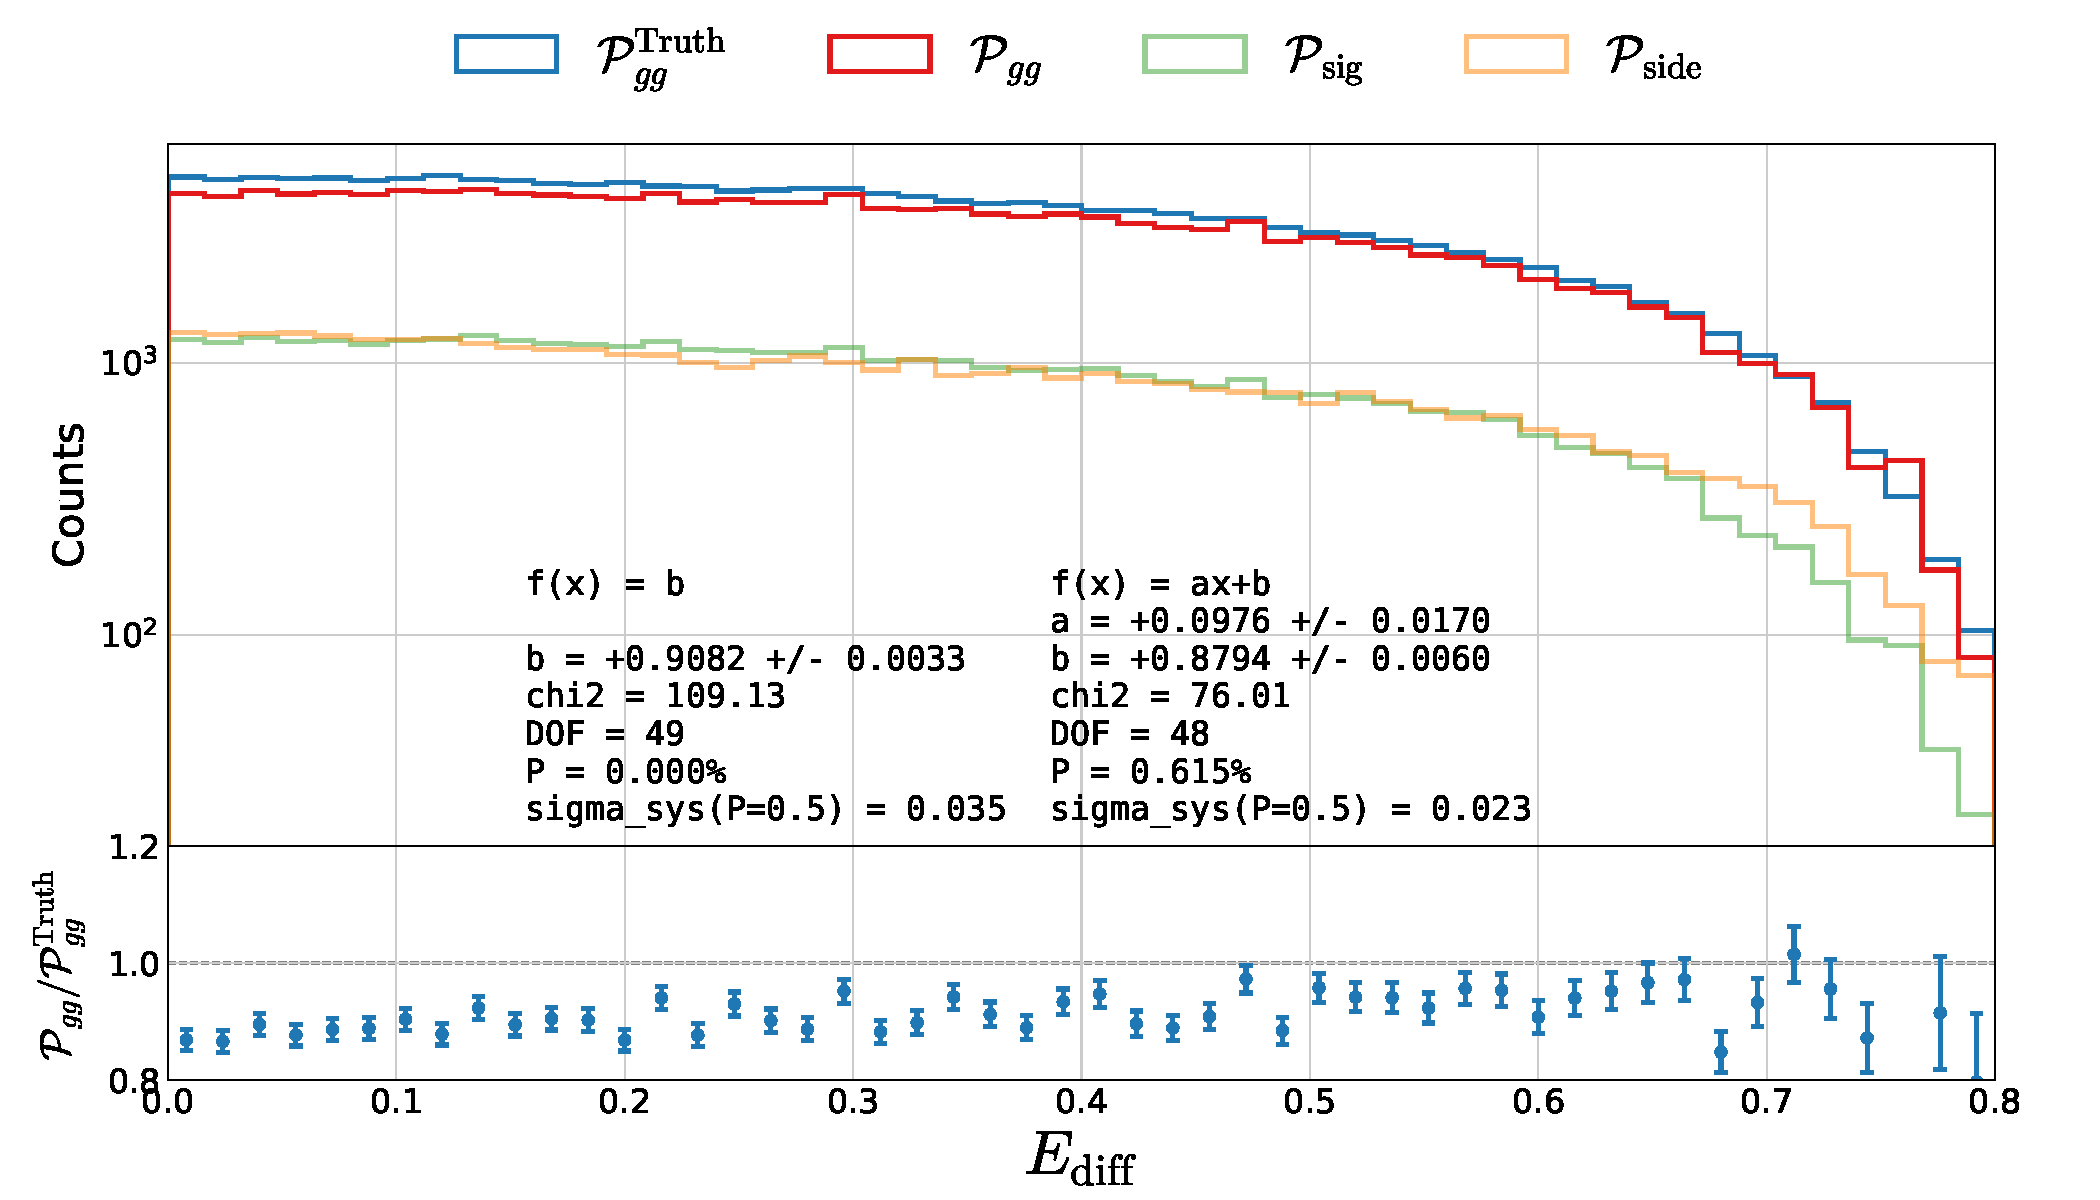
\includegraphics[width=0.99\textwidth, trim=10 0 20 5, clip, page=1]{figures/quarks/gtag-closure_test-down_sample=1.00-ML_vars=vertex-selection=b-ejet_min=4-n_iter_RS_lgb=99-n_iter_RS_xgb=9-cdot_cut=0.90-version=19-njet=4.pdf}
  \caption[Closure Plot Comparing MC Truth and the Efficiency Corrected $g$-Tagging Model in 4-Jet Events for the Normalized Gluon Gluon Jet Energy Asymmetry]
          {Closure plot comparing MC Truth and the efficiency corrected $g$-tagging model in 4-jet events for the normalized gluon gluon jet energy asymmetry $E_\mathrm{diff}$. In the top part of the plot \textcolor{blue}{$\mathcal{P}_{gg}^\mathrm{Truth}$} based on MC Truth is shown in blue, the \textcolor{red}{$\mathcal{P}_{gg}$} based on MC but without Truth in red, the distribution in the signal region \textcolor{green}{$\mathcal{P}_{\mathrm{sig}}$} in light green and the distribution in the sideband region \textcolor{orange}{$\mathcal{P}_{\mathrm{side}}$} in light orange. In the bottom part of the plot the ratio between $\mathcal{P}_{gg}$ and $\mathcal{P}_{gg}^\mathrm{Truth}$  is shown. 
          } 
  \label{fig:q:closure_E_diff_non_appendix}
\end{figure}

The errorbars in the ratio plot are fitted with both a constant $f(x)=b$ and a straight line $f(x)=ax+b$ with the fit results shown as text in the plot. The closure plot for the rest of the gluon splitting variables in Figure~\ref{fig:q:closure_E_diff}--\ref{fig:q:closure_variable_pt_antenna}. In general it can be seen that the $\mathcal{P}_{gg}$ matches $\mathcal{P}_{gg}^\mathrm{Truth}$ pretty well for all the gluon splitting variables, however, with a \SI{10}{\percent} offset. This offset is easy to correct for with a constant correction factor. 

However, we see that for the energy asymmetry variables and $\Delta_\theta$ there are clear, linear trends in the ratio plots. This is seen e.g. for $E_\mathrm{diff}$ in Figure~\ref{fig:q:closure_E_diff_non_appendix} where the $\chi^2$ value for the constant fit is \num{109.13} but only \num{76.01} for the linear fit. This difference in $\chi^2$ value cannot be attributed to just the linear fit being a more advanced fit in which case the difference would be expected to be $\Delta \chi^2 \sim 1$ due to difference in the number of fit parameters being \num{1}. For these four variables the systematic uncertainty will thus be based on the linear fit, whereas it will be based on the constant for the rest of the variables. 

The $g$-tagging algorithm perform well in general where most of the systematic attributed are \SI{2}{\percent} to \SI{3}{\percent}. The highest systematic uncertainty is for the invariant mass of the two gluons: $\sigma_\mathrm{sys}(m_{gg}) = \SI{3.6}{\percent}$. A summary of all the systematic errors from the closure tests can be seen in Table~\ref{tab:q:gluon_splitting_systematic_errors} for all of the gluon splitting variables. 

\begin{margintable}[-3cm]
  \centerfloat
  \begin{tabular}{@{}rrc@{}}
  {}                                                & $\sigma_\mathrm{sys}$& $f(x)$ \\ \addlinespace[0.1em] \midrule \addlinespace[0.2em]
  $E_\mathrm{diff}$                                 & $\SI{2.3}{\percent}$ & $ax+b$ \\ \addlinespace[0.2em]
  $E_{\mathrm{rel}_\mathrm{min}}$                   & $\SI{2.3}{\percent}$ & $ax+b$  \\\addlinespace[0.2em]
  $E_\mathrm{rel}$                                  & $\SI{2.5}{\percent}$ & $ax+b$  \\\addlinespace[0.2em]
  $\Delta_\theta$                                   & $\SI{2.0}{\percent}$ & $ax+b$  \\\addlinespace[0.2em]
  $m_{gg}$                                          & $\SI{3.6}{\percent}$ & $b$ \\\addlinespace[0.2em]
  $\phi_\mathrm{\parallel}$                         & $\SI{1.7}{\percent}$ & $b$  \\\addlinespace[0.2em]
  $\ln \left( k_t^2 / m_\mathrm{vis}^2 \right)$     & $\SI{2.1}{\percent}$ & $b$ \\\addlinespace[0.2em]
  $p^2_{\perp,\mathrm{A}}$                          & $\SI{3.1}{\percent}$ & $b$  \\ %\bottomrule
  \end{tabular}
  \vspace{3mm}
  \caption[Gluon Splitting Systematic Errors]{\label{tab:q:gluon_splitting_systematic_errors}Systematic errors for the gluon splitting variables based on the closure test, see \autoref{subsec:q:gluon_splitting_closure}.  The last column, $f(x)$, denotes which fit the systematic error is based on.}
\end{margintable}


The closure test shows that the $g$-tagging algorithm can also be trusted in the 4-jet case, however, with high systematic uncertainties for the $m_{gg}$ variable. 

\subsection{Results}
\label{subsec:q:gluon_splitting_results}

\begin{margintable}[1cm]
  \centerfloat
  \begin{tabular}{@{}ccc@{}}
  Region  & $R_{gg}^{k_t}$                & $R_{gg}^\mathrm{CA}$    \\ \addlinespace[0.1em] \midrule \addlinespace[0.4em]
  A       & $[0, 1]$                      & $[0, 1]$                \\ \addlinespace[0.4em]
  B       & $[\frac{3}{5}, \frac{5}{3}]$  & $[\frac{3}{5}, \frac{5}{3}]$            \\ \addlinespace[0.4em]
  C       & $[0, \frac{5}{3}]$            & $[1, \infty]$           \\ \addlinespace[0.4em]
  D       & $[\frac{5}{3}, \infty]$       & $[\frac{5}{3}, \infty]$
  \end{tabular}
\vspace{3mm}
\caption[Rgion Definition in the $R_{gg}^{k_t}$-$R_{gg}^\mathrm{CA}$ Phase Space]{\label{tab:q:gluon_splitting_region_definitions}Definitions of the four regions in the $R_{gg}^{k_t}$-$R_{gg}^\mathrm{CA}$ phase space.}
\end{margintable}

The comparison between the gluon splitting distributions will be done in four distinct regions of the $R_{gg}^{k_t}$-$R_{gg}^\mathrm{CA}$ phase space. These four regions, A, B, C, and D, are defined in Table~\ref{tab:q:gluon_splitting_region_definitions}. Three of these regions have already been described, that is region A which is the soft, collinear region with an example shown in Figure~\ref{fig:q:kt_CA_soft_collinear}, region C which is the soft, wide angle region in Figure~\ref{fig:q:kt_CA_soft_wide}, and the hard non-($g\rightarrow gg$) region D in Figure~\ref{fig:q:kt_CA_hard_non_g_to_gg}. Region B is a region where neither the $k_t$ algorithm nor the CA algorithm is totally sure whether or not the two gluons should be clustered together. 

The four regions are visualized in Figure~\ref{fig:q:R_kt_CA_overview} for both MC and Data. Here each dot shown in the scatter plot is an event with $0.8 < \gamma_\mathrm{tag}$, totalling \num{41117} events in the MC sample and \num{22473} events in the data sample. The number of events that fall into each of the four regions are shown in the figure. The events are split up into these four regions because they each concern different physical interactions. The number of events in each region were taken into account when creating the ranges in Table~\ref{tab:q:gluon_splitting_region_definitions} to minimize the statistical uncertainties. 

\begin{figure*}[h!]
  \centerfloat
  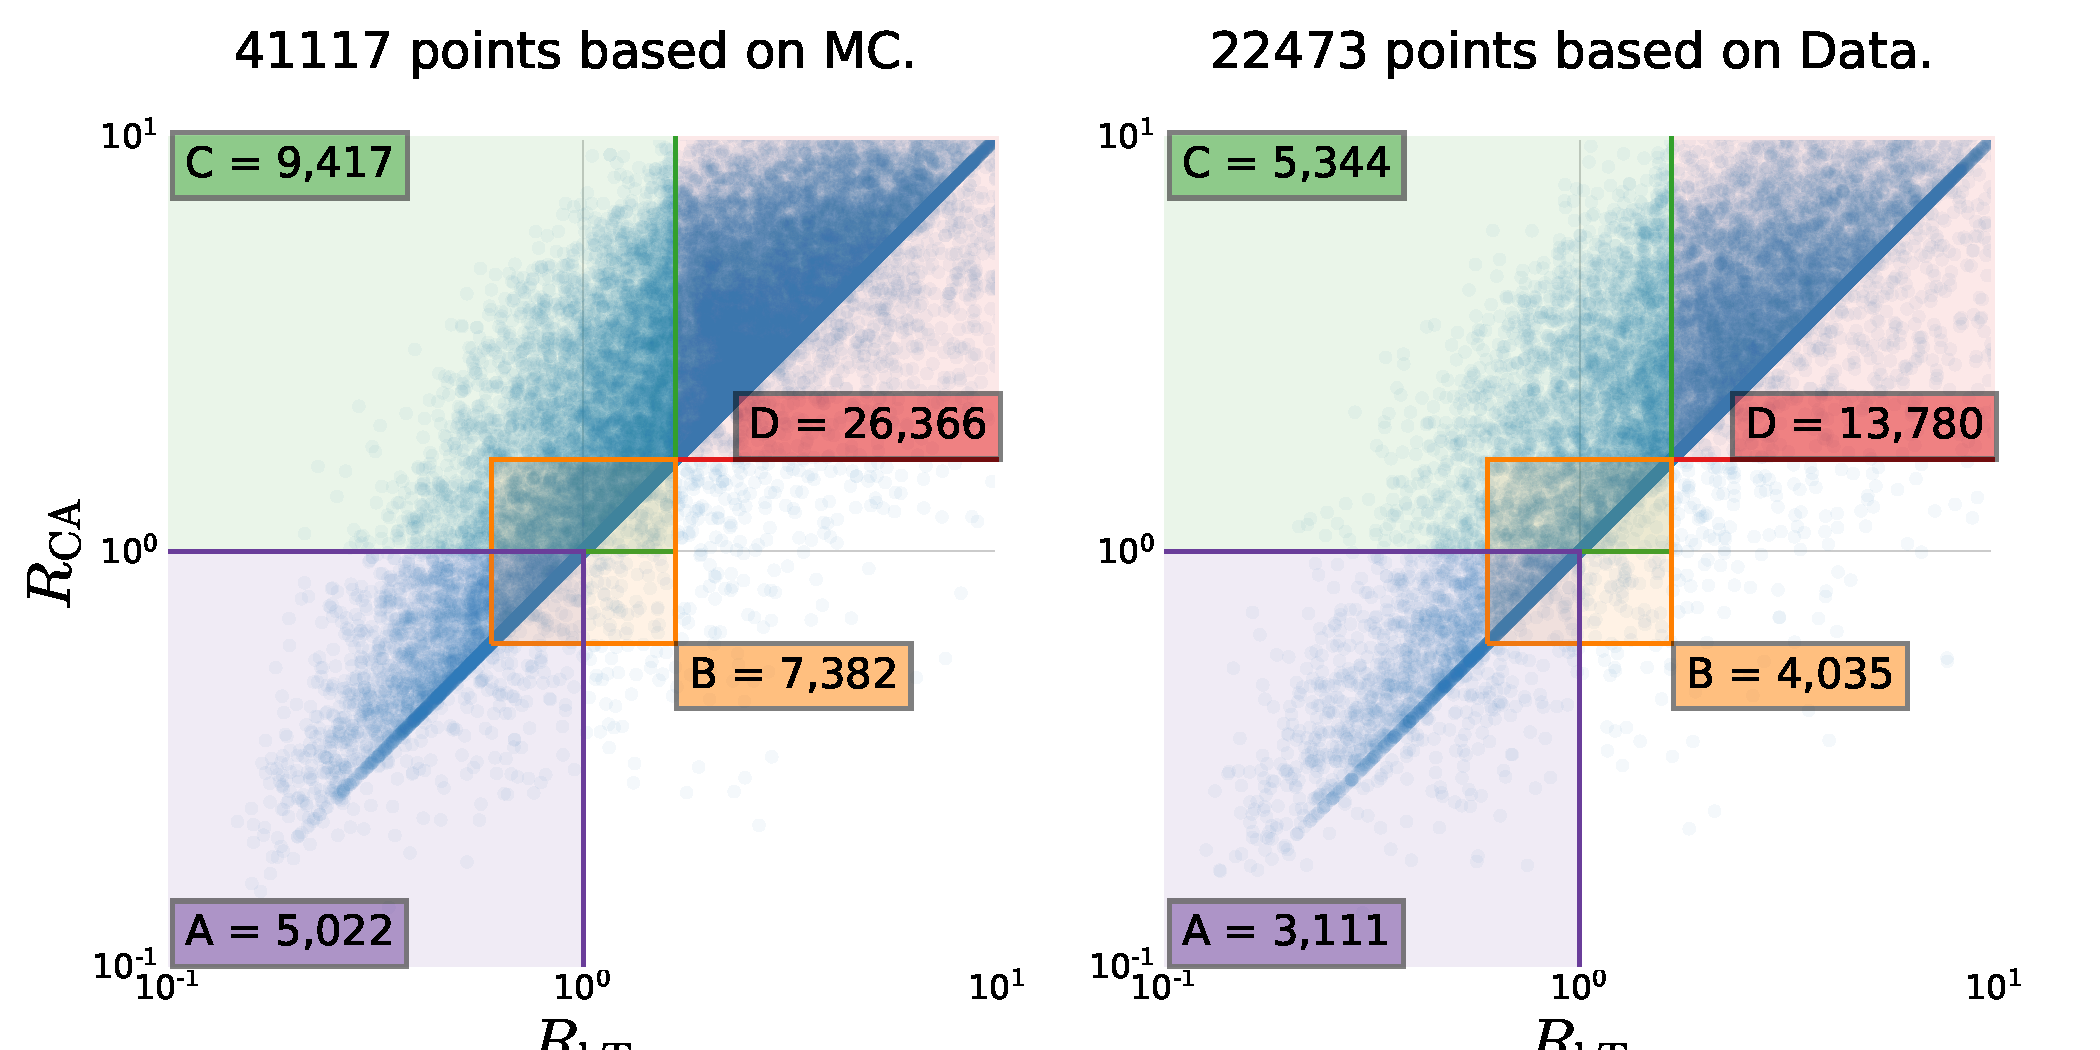
\includegraphics[width=0.95\textwidth, trim=0 0 0 0, clip]{figures/quarks/gtag-R_kt_CA_overview-down_sample=1.00-ML_vars=vertex-selection=b-ejet_min=4-n_iter_RS_lgb=99-n_iter_RS_xgb=9-cdot_cut=0.90-version=19-njet=4.pdf}
  \caption[Overview of the Four Regions in the $R_{gg}^{k_t}$-$R_{gg}^\mathrm{CA}$ Phase Space]
          {Overview of the four regions, A, B, C, and D, in the $R_{gg}^{k_t}$-$R_{gg}^\mathrm{CA}$ phase space. The regions are shown as colored rectangles together with a scatter plot showing the 2D-distribution for signal gluon events ($0.8 < \gamma_\mathrm{tag}$). The left plot shows is for MC and the right one for Data.} 
  \label{fig:q:R_kt_CA_overview}
\end{figure*}
% \vspace{-3mm}

The distributions for the different gluons splitting variables for region A, the soft, collinear region, is shown in Figure~\ref{fig:q:R_kt_CA_cut_A_non_appendix} for both MC (scaled to Data) and Data. The in addition to scaling MC to Data, the samples have been efficiency corrected in the histograms, that is given a weight $w(x)=1/ \varepsilon_{gg}^{4\dash\mathrm{jet}}(x)$. Region A contains \num{5022} events in the MC sample and \num{3111} in the Data samples. Generally the distributions match pretty well between the MC and Data, however, there seems to be small discrepancies in the energy asymmetry variables, however, this might just be due to statistical fluctuations (notice the low bin count in each bin). 

\begin{figure*}[h!]
  \centerfloat
  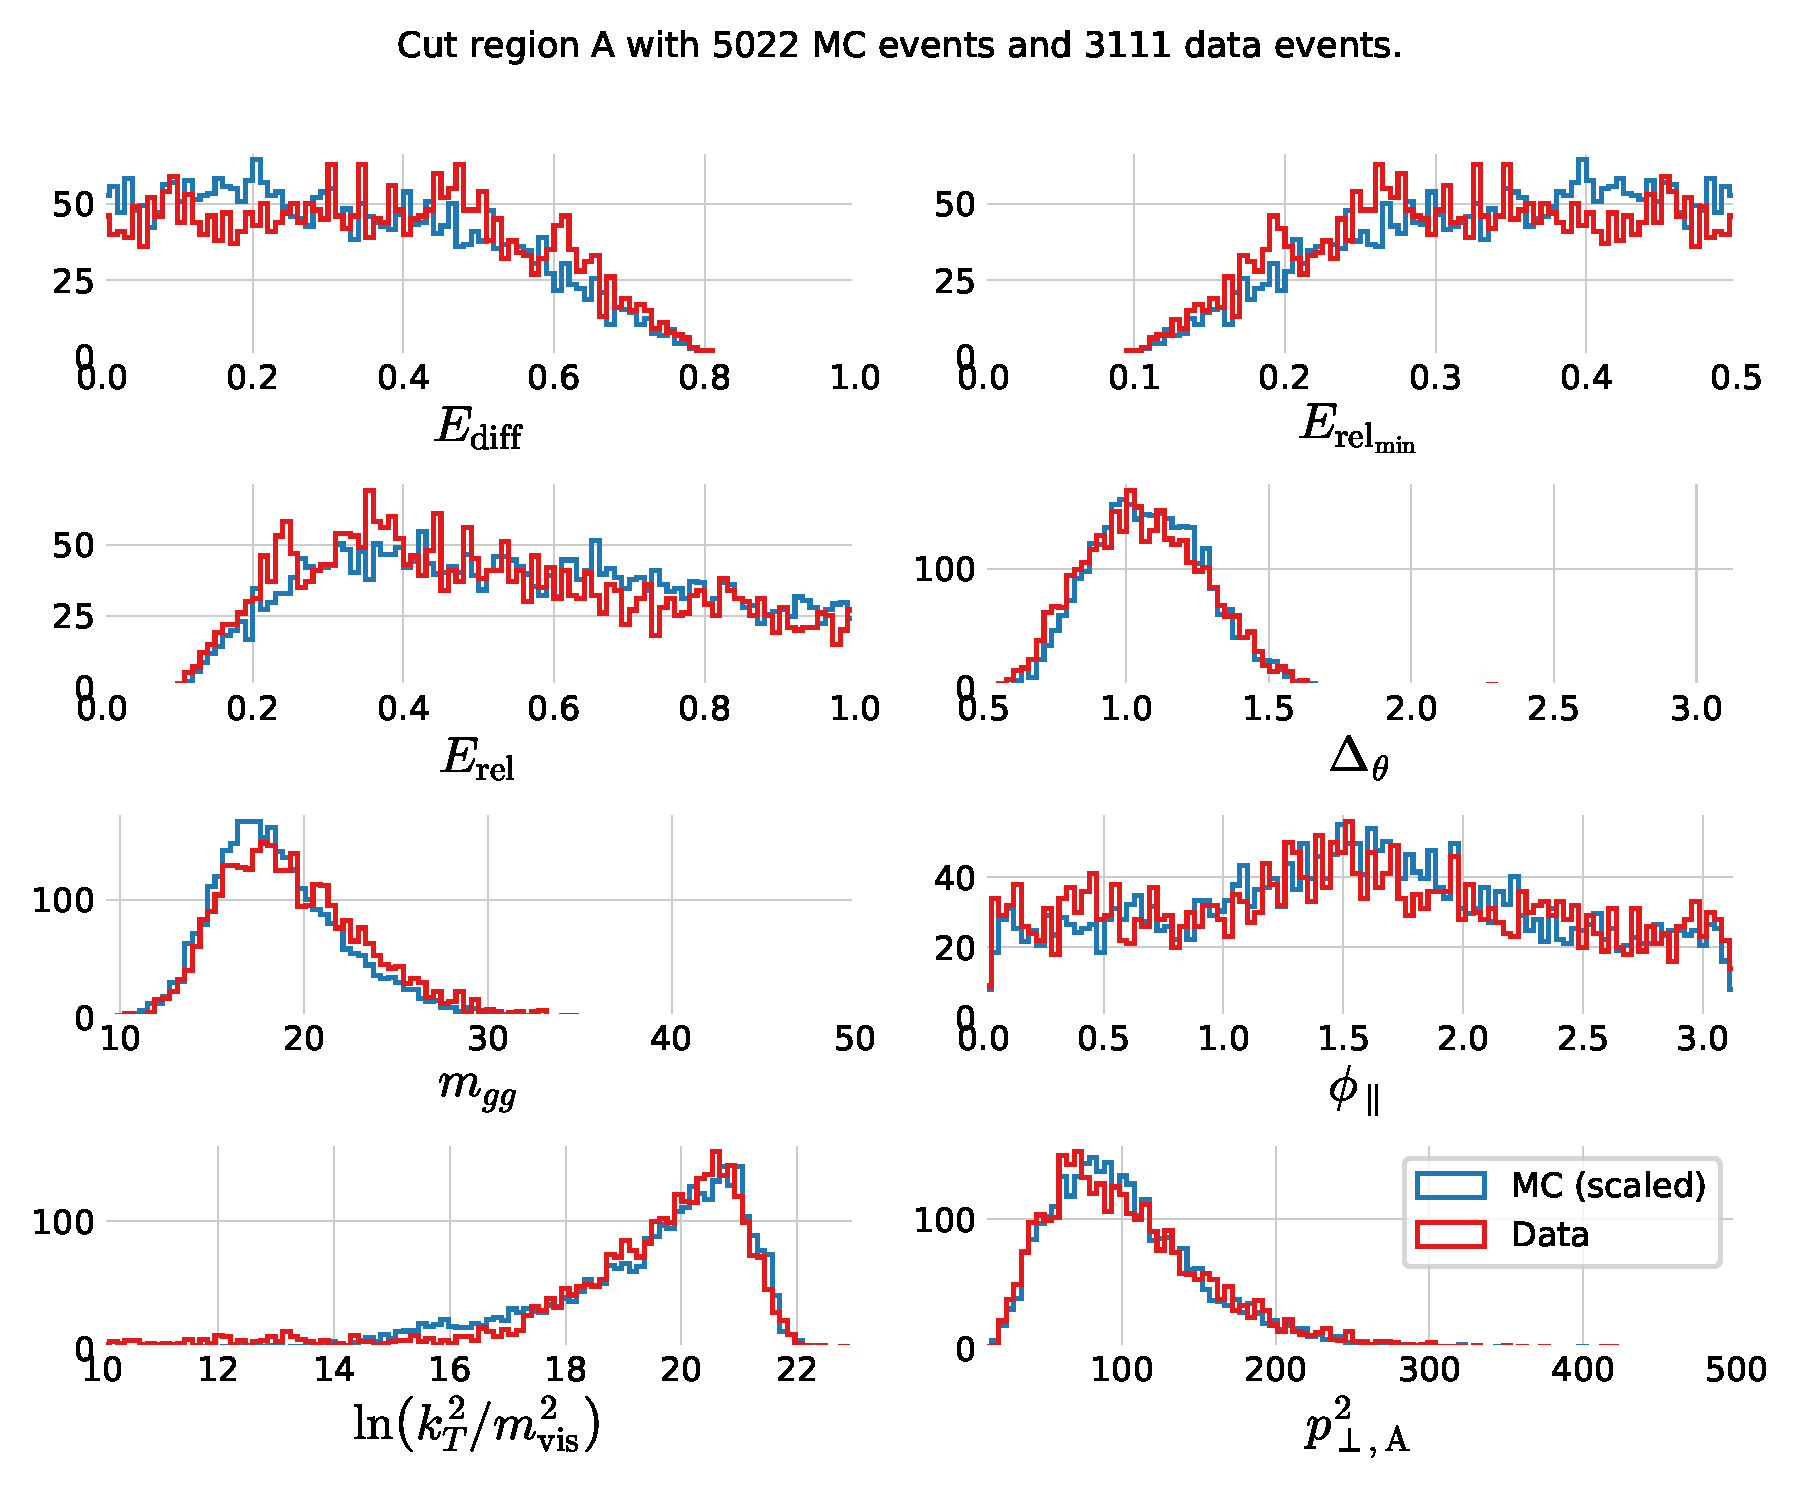
\includegraphics[width=0.99\textwidth, trim=0 0 0 0, clip]{figures/quarks/gtag-R_kt_CA_histograms-down_sample=1.00-ML_vars=vertex-selection=b-ejet_min=4-n_iter_RS_lgb=99-n_iter_RS_xgb=9-cdot_cut=0.90-version=19-njet=4.pdf}
  \caption[Gluon Splitting Distribution Comparison in MC and Data for $R_{gg}^{k_t}$-$R_{gg}^\mathrm{CA}$ Phase Space Region A]
          {Comparison of the gluon splitting distributions in MC and Data for $R_{gg}^{k_t}$-$R_{gg}^\mathrm{CA}$ phase space region A, see Table~\ref{tab:q:gluon_splitting_region_definitions}. The distribution for \textcolor{blue}{MC} (scaled to Data) is shown in blue and for \textcolor{red}{Data} in red. Both MC and Data has been efficiency corrected. These eight distributions are for the $R_{gg}^{k_t}$-$R_{gg}^\mathrm{CA}$ region A which has \num{5022} events in the MC sample and \num{3111} in the Data sample. } 
  \label{fig:q:R_kt_CA_cut_A_non_appendix}
\end{figure*}

When looking at the other regions, see Figure~\ref{fig:q:R_kt_CA_cut_A}--\ref{fig:q:R_kt_CA_cut_D}, the energy discrepancies seem to disappear. To compare the similarity of the MC and Data distributions, I perform a Kolmogorov–Smirnov (KS) two-sample test. This nonparametric hypothesis test compares two samples based on the null hypothesis that they are both samples coming from the same (but unknown) parent distribution. The KS test outputs the probability $P_\mathrm{KS}$ of the null hypothesis. I add this probability to the plot if it is less than \SI{100}{\percent}. This is only the case in region D, Figure~\ref{fig:q:R_kt_CA_cut_D}, which I suspect is due to low statistics in the other regions as the KS test is known for its low power \autocite{mohdrazaliPowerComparisonsShapiroWilk2011}. 

To properly test the assumption that the variations in $E_\mathrm{diff}$ are due to statistical noise, I make a ratio plot between MC and Data and compare them between region A and D. The plot for region A is shown in Figure~\ref{fig:q:ratio_plot_E_diff_region_A}. When looking at the ratio plot in the bottom part of the figure, it can be seen that the almost all of the bins are with $1\sigma$ of \num{1}. Indeed, when calculating the $\chi^2$ value between the errorbars and a constant ratio of \num{1}, that is to say $f(x)=1$, one finds a $\chi^2$ probability of $P_{\chi^2}=\SI{51.3}{\percent}$. This value strongly suggests that the fluctuations in the two histograms are due to statistical noise (at least we cannot disprove that it is not). Remember, that this was not even a fit, but simply a comparison to a (fixed) constant. 

\begin{figure}[h!]
  \centerfloat
  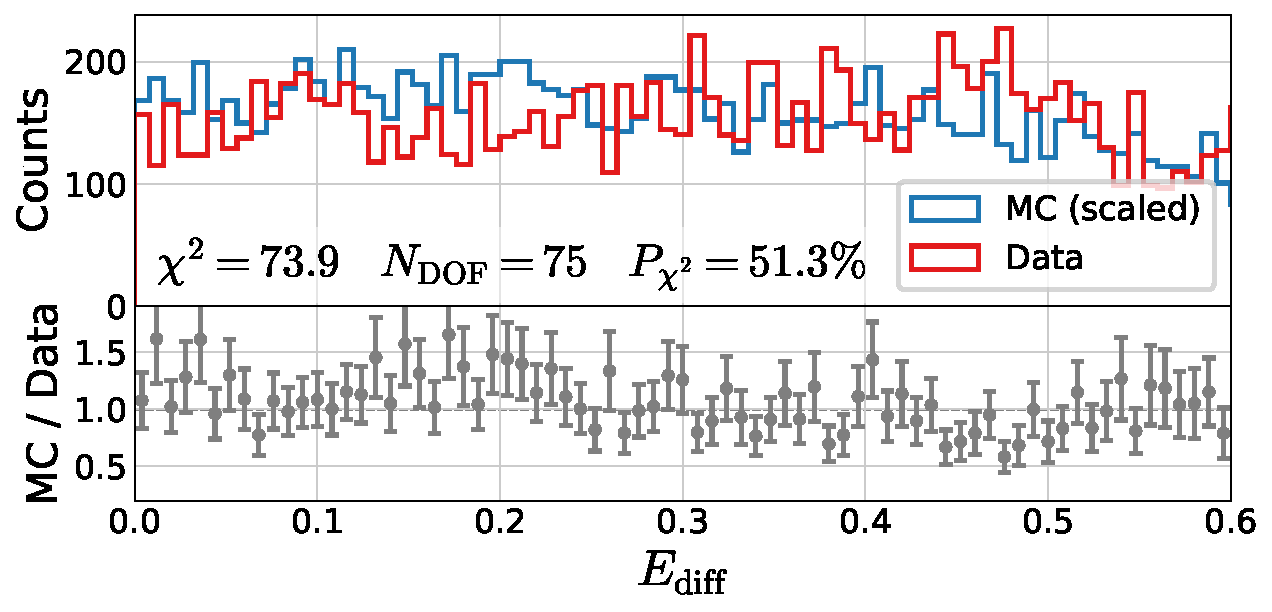
\includegraphics[width=0.99\textwidth, trim=0 0 0 0, clip]{figures/quarks/cut_region_A_ratio_plot-down_sample=1.00-ML_vars=vertex-selection=b-ejet_min=4-n_iter_RS_lgb=99-n_iter_RS_xgb=9-cdot_cut=0.90-version=19-njet=4.pdf}
  \caption[Ratio Plot of $E_\mathrm{diff}$ in MC and Data for $R_{gg}^{k_t}$-$R_{gg}^\mathrm{CA}$ for Region A]
          {Ratio plot of the gluon splitting variable $E_\mathrm{diff}$ in MC and Data for $R_{gg}^{k_t}$-$R_{gg}^\mathrm{CA}$ in region A. In the top plot, the distribution of $E_\mathrm{diff}$ for \textcolor{blue}{MC} (scaled to Data) is shown in blue and for \textcolor{red}{Data} in red. Both MC and Data has been efficiency corrected. Below are the ratio plot between MC and Data. In text is written the $\chi^2$ between the errorbars and a constant ratio equal to \num{1}. That is to say that $f(x)=1$, which is thus not a fit. The $\chi^2$ probability is written as $P_{\chi^2}$ and it indicates an almost perfect correspondence between Data and MC.} 
  \label{fig:q:ratio_plot_E_diff_region_A}
\end{figure}

In Figure~\ref{fig:q:ratio_plot_E_diff_region_D} one can compare the ratio in region A with the one in region D. Even though region D contains a lot more data, the same pattern is seen as for region A. In region D the $\chi^2$ probability is even a bit too high which indicates too little variation between the two histograms, however, not by too much to just happen by chance. In comparison to the $\chi^2$ probability, the KS probability between the two samples is $P_\mathrm{KS}(E_\mathrm{diff})=\SI{0.25}{\percent}$. This difference in probability is an implication of the fact that the KS test and $\chi^2$ test are sensitive to different characteristics, e.g. the $\chi^2$ test is only sensitive to absolute differences between distributions, whereas the KS test is not bound to only compare absolute differences. 

\begin{figure}
  \centerfloat
  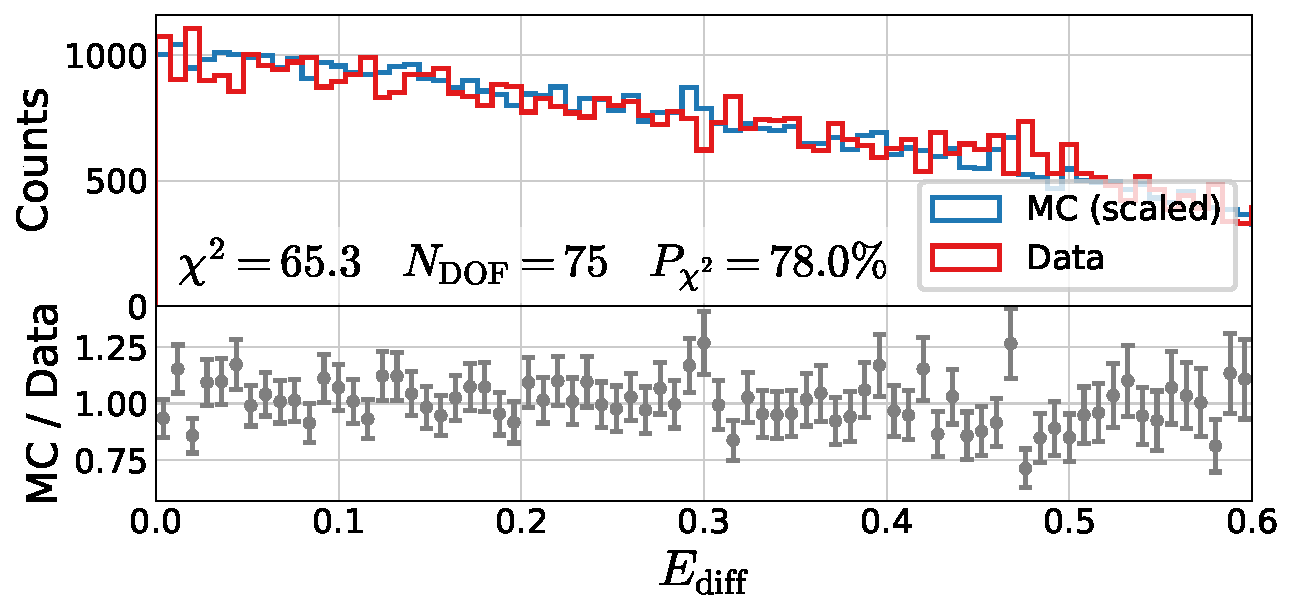
\includegraphics[width=0.99\textwidth, trim=0 0 0 0, clip]{figures/quarks/cut_region_D_ratio_plot-down_sample=1.00-ML_vars=vertex-selection=b-ejet_min=4-n_iter_RS_lgb=99-n_iter_RS_xgb=9-cdot_cut=0.90-version=19-njet=4.pdf}
  \caption[Ratio Plot of $E_\mathrm{diff}$ in MC and Data for $R_{gg}^{k_t}$-$R_{gg}^\mathrm{CA}$ for Region D]
          {Ratio plot of the gluon splitting variable $E_\mathrm{diff}$ in MC and Data for $R_{gg}^{k_t}$-$R_{gg}^\mathrm{CA}$ in region D. In the top plot, the distribution of $E_\mathrm{diff}$ for \textcolor{blue}{MC} (scaled to Data) is shown in blue and for \textcolor{red}{Data} in red. Both MC and Data has been efficiency corrected. Below are the ratio plot between MC and Data. In text is written the $\chi^2$ between the errorbars and a constant ratio equal to \num{1}. That is to say that $f(x)=1$, which is thus not a fit. The $\chi^2$ probability is written as $P_{\chi^2}$ and it indicates an high correspondence between Data and MC, almost too high.} 
  \label{fig:q:ratio_plot_E_diff_region_D}
\end{figure}

In general there seems to be a high degree of correspondence between the distributions for MC and Data for all the gluon splitting variables in all four of the regions of phase space tested. 



\section{Discussion}
\label{sec:q:discussion}

The distributions of both the generalized angularities and the gluon splitting variables are based on the $g$-tagging model which itself is based on the $b$-tagging model. At first this way of training two different ML models, where one is trained on the other\sidenote{This is very different to the ensemble model used in \autoref{sec:h:multiple_models} which can basically be treated as a single, advanced ML model.}, might seem a bit counterintuitive: why not just build a single, combined model that is able to extract gluons? The reason why the method used here is set up the way it is, is to be able to better understand the intermediate steps while also being able to compare the results to others. With the $b$-tagging model we are able to compare our model to the neural network trained by ALEPH (NNB) and measure the $b$-tagging efficiency for both gluons and $b$-quarks individually. Neither of these would not have been possible with a combined model which just outputs single gluons. 

Regarding the NNB model, it is interesting to compare the $b$-tagging ROC curves in Figure~\ref{fig:q:roc_btag_4j} for 4-jets and \ref{fig:q:roc_btag_3j} for 3-jets. Even thought the performance for the old NNB model is comparable to our model\sidenote{Technically models, both the XGBoost model and the LightGBM model.}, especially for 3-jet events, one has to take into account that the NNB model is trained on nine variables compared to only three variables by our model. Yet, remember that this is a model that was trained more than \num{25} years ago by now. I doubt many other areas of science implemented machine models that long ago with a performance that is almost comparable to today's.

That we only train on the vertex variables is to reduce any potential bias that might be introduced when training on the shape variables (in addition to the vertex variables) and then afterwards used to compare the same shape variables between MC and Data afterwards. Another approach to this would be to train on all variables and then afterwards quantify the potential bias and correct for it. This would also allow one to compare the loss in performance by only using the vertex variables. This was not done in this project due to time limitations.

As mentioned above, with the modularized approach we apply in this project we are able to measure the $b$-tagging efficiencies not only in MC but also in Data. The efficiencies were measured using a tag-tag-probe method in 3-jet events. In 4-jet events this problem is a lot harder, however, it might have been possible to apply a tag-tag-tag-probe method, although the results of this are very likely to be limited by large uncertainties due to much lower statistics in 4-jet events compared to 3-jet events. 

Some sources of error in this project not yet mentioned are the fact that we do not have access to the full MC simulation and that sometimes particles do not get detected in the detector. That we do not have access to the full MC simulation means that we have to $q$-matching to the final quarks; we do not know the real truth for the jets, even in MC. On the other hand, particles going undetected is something that also happens i Data. When this happens in e.g. a 4-jet event it will be classified as a 3-jet event in the data which it was clearly not originally. 

Even after taking the sources of error into account along with the statistical and systematic errors, the result would still not reflect Nature. This is due to the fact that the observations $g(y)$ are a combination of the truth in Nature $f(x)$ combined with the detector $A(x, y)$. This combination is mathematically a convolution \autocite{schmittDataUnfoldingMethods2017}: 
\begin{equation}
  \label{eq:q:convolution}
  \int f(x) A(x, y) \mathop{dx} = g(y).
\end{equation}
The goal is thus to estimate truth $f(x)$ given knowledge about the detectors response $A(x,y)$. Another way to look at this is that $f(x)$ is smeared, or distorted, by detector and binning effects (e.g. finite resolutions). The process of inverting equation \eqref{eq:q:convolution} is known as \emph{unfolding} and is basically a deconvolution process. 

\section{Conclusion}
\label{sec:q:conclusion}

XXX \TODO